% Standalone editable source. No external figures or custom font files required.
% Build twice with: pdflatex -interaction=nonstopmode -halt-on-error solver_routing.tex
% Original specification and vector TikZ diagrams authored by GPT Pro.
% Subsequent implementation verification and policy amendments are authored by Codex.
% The direct-cost amendment follows an actual GPT Pro review on 14 October 2026.
% The allocation amendment uses a generic Pro methodology review, not project approval.
\documentclass[11pt,letterpaper]{article}
\usepackage[margin=0.67in,top=0.72in,bottom=0.67in,headheight=14pt,headsep=14pt]{geometry}
\usepackage[T1]{fontenc}
\usepackage{lmodern,microtype}
\usepackage{amsmath,amssymb,array,tabularx,booktabs}
\usepackage[table]{xcolor}
\usepackage{tikz}
\usetikzlibrary{arrows.meta,positioning,calc,shapes.geometric,fit,backgrounds}
\usepackage[most]{tcolorbox}
\usepackage{enumitem,fancyhdr,lastpage,ragged2e}
\usepackage{hyperref}
\definecolor{Ink}{HTML}{203149}
\definecolor{Teal}{HTML}{096D73}
\definecolor{Muted}{HTML}{536478}
\definecolor{Pale}{HTML}{EDF5F5}
\definecolor{Light}{HTML}{F3F5F8}
\definecolor{Rule}{HTML}{CAD5DE}
\definecolor{Amber}{HTML}{86570C}
\definecolor{Warm}{HTML}{FAF4E8}
\hypersetup{colorlinks=true,linkcolor=Teal,urlcolor=Teal,pdftitle={Efficient FE solver routing},pdfauthor={GPT Pro; subsequent amendments and verification by Codex},pdfsubject={Mapped native checks passed; performance evidence blocks adoption},pdfkeywords={fixed effects, solver routing, CMG, within, deterministic controller}}
\pagestyle{fancy}
\fancyhf{}
\fancyhead[L]{\sffamily\fontsize{8.5}{10}\selectfont\color{Muted}FEREG / ENGINEERING SPECIFICATION}
\fancyhead[R]{\sffamily\fontsize{8.5}{10}\selectfont\color{Muted}REVISED 16 OCTOBER 2026}
\fancyfoot[L]{\sffamily\fontsize{8}{10}\selectfont\color{Muted}Mapped native checks passed / performance adoption blocked}
\fancyfoot[R]{\sffamily\fontsize{8.5}{10}\selectfont\color{Ink}\thepage\ / \pageref*{LastPage}}
\renewcommand{\headrulewidth}{0.3pt}
\renewcommand{\footrulewidth}{0pt}
\setlength{\parindent}{0pt}
\setlength{\parskip}{4.0pt}
\setlength{\tabcolsep}{5.5pt}
\renewcommand{\arraystretch}{1.16}
\setlist[itemize]{leftmargin=13pt,itemsep=2pt,topsep=3pt,parsep=0pt}
\setlist[enumerate]{leftmargin=17pt,itemsep=2pt,topsep=3pt,parsep=0pt}
\newcolumntype{Y}{>{\RaggedRight\arraybackslash}X}
\newcolumntype{P}[1]{>{\RaggedRight\arraybackslash}p{#1}}
\newcommand{\body}{\fontsize{10.5}{13.45}\selectfont\color{Ink}\RaggedRight}
\newcommand{\smallbody}{\fontsize{9.4}{11.65}\selectfont\color{Ink}\RaggedRight}
\newcommand{\tinybody}{\fontsize{8.6}{10.6}\selectfont\color{Ink}\RaggedRight}
\newenvironment{compactleaf}{\setlength{\parskip}{2.5pt}\renewcommand{\arraystretch}{1.06}\renewcommand{\smallbody}{\fontsize{9.2}{11.1}\selectfont\color{Ink}\RaggedRight}\renewcommand{\sub}[1]{\par\vspace{2pt}{\sffamily\bfseries\fontsize{11.5}{14}\selectfont\color{Teal}##1\par}}\renewcommand{\tagline}[1]{{\sffamily\fontsize{9.5}{12}\selectfont\color{Muted}##1\par}\vspace{3pt}}}{}
\newcounter{specsection}
\newcommand{\sect}[2]{\stepcounter{specsection}\pdfbookmark[0]{#2}{spec.\arabic{specsection}}\vspace*{1pt}{\sffamily\bfseries\color{Teal}\fontsize{9}{11}\selectfont #1\par}\vspace{4pt}{\sffamily\bfseries\color{Ink}\fontsize{21}{24}\selectfont #2\par}\vspace{8pt}}
\newcommand{\sub}[1]{\par\vspace{4pt}{\sffamily\bfseries\fontsize{11.5}{14}\selectfont\color{Teal}#1\par}\vspace{1pt}}
\newcommand{\tagline}[1]{{\sffamily\fontsize{9.5}{12}\selectfont\color{Muted}#1\par}\vspace{5pt}}
\newcommand{\code}[1]{\texttt{#1}}
\newcommand{\anchor}[1]{\par\vspace{2pt}{\fontsize{8.6}{10.7}\selectfont\color{Muted}\textbf{Source anchor:} #1\par}}
\newtcolorbox{note}[1][]{colback=Pale,colframe=Teal,boxrule=0pt,leftrule=2.5pt,arc=0pt,left=9pt,right=9pt,top=6pt,bottom=6pt,before skip=7pt,after skip=7pt,#1}
\newtcolorbox{binding}[1][]{colback=Warm,colframe=Amber,boxrule=0pt,leftrule=2.5pt,arc=0pt,left=9pt,right=9pt,top=6pt,bottom=6pt,before skip=7pt,after skip=7pt,#1}
\newcommand{\rowhead}{\rowcolor{Ink}\color{white}\bfseries}
\newcommand{\newleaf}{\newpage\body}
\newcommand{\algline}[2]{\textcolor{Muted}{\makebox[17pt][r]{\scriptsize #1}}\hspace{6pt}#2\par}
\begin{document}
\body

% PAGE 1 ----------------------------------------------------------------------
\thispagestyle{fancy}\pdfbookmark[0]{Overview}{overview}
{\sffamily\bfseries\fontsize{10}{12}\selectfont\color{Teal}IMPLEMENTATION SPECIFICATION\par}
\vspace{8pt}
{\sffamily\bfseries\fontsize{32}{35}\selectfont Efficient FE\par solver routing\par}
\vspace{6pt}
{\sffamily\fontsize{13}{17}\selectfont\color{Muted}Integrated experimental contract;\par mapped native checks passed; performance adoption blocked\par}
\vspace{3pt}
{\sffamily\fontsize{10.5}{14}\selectfont 13 October 2026 / amended through 16 October 2026\par}
\vspace{6pt}
\begin{note}
\textbf{Design in one sentence.} Keep \code{auto} as a small deterministic router: exact structural shortcuts, inexpensive incumbent iterations, and at most one bounded optional upgrade, followed by an independent original-problem certificate.
\end{note}
\sub{Purpose and implementation boundary}
Serial routing, overlap, prefix arms and PPML topology sharing are implemented. The explicit-CMG repair passes its full suite and fresh native checks (page 16); untimed routing prerequisites pass (page 15). Authorized recovery now passes all 20 standard cells (page 21). Original timing outcomes remain on pages 18--20; ablation timings are exploratory and policy A replacements remain ineligible. Ordinary \code{auto} and explicit IT remain unchanged. No routing policy is selected or promoted.
\sub{Scientific and runtime invariants}
Preserve explicit solver contracts, unsafe-CG rejection, supported OLS/PPML requests and both bias modes. Existing authorities decide sample membership, rank, omissions and separation; preserve original factor slots and base flags. Routing, factor pivots and numerical preconditioners must not redefine those decisions.

Use one native call. SPI stays on the main thread; workers own Rust-managed state. Break checks, deterministic error arbitration, joining and atomic rollback apply before publication. No uncertified best-so-far output may be published. Exact operators mean the original mathematical problem, not an absence of floating-point error.
\sub{Reading map}
{\smallbody
\begin{tabularx}{\linewidth}{P{0.49\linewidth}Y}
\toprule
\textbf{Architecture and execution} & \textbf{Integration and release}\\
\midrule
2 Frontier and frozen policy constants & 8 Controlled builder and worker ownership\\
3 Routing flowchart & 9 Parallel grant timeline and terminal handling\\
4 Types, sessions and native iteration limits & 10 Staged delivery, prefixes and PPML\\
5 Deterministic work and memory admission & 11 Statistical performance qualification\\
6 Executable serial controller & 12 Verification, bindings and source anchors\\
7 Exact two-FE and within-CMG contracts & 13 Current implementation bindings (Codex)\\
 & 14 Reviewed direct-cost amendment (Codex)\\
 & 15 Evidence and experimental boundaries (Codex)\\
16 CMG repair; 17 deployment (Codex) & 18--21 Timing history and recovery (Codex)\\
\bottomrule
\end{tabularx}}
{\tinybody\color{Teal}\textbf{Private policy:} pages 23--26. SCC NO-GO: page 27. Diagnosis: pages 28--31. Next discovery: page 32. Public Auto unchanged.\par}
\vfill
{\fontsize{9}{11.8}\selectfont\color{Muted}\textbf{Authorship.} GPT Pro authored the original specification and diagrams. Codex authored later bindings and amendments. Exact-case Pro review informed the direct-cost correction (page 14); generic Pro review informed allocation (page 8). The explicit-CMG repair (page 16) is a Codex amendment, not GPT Pro code approval.\par
Document rendering and layout validation do not constitute solver implementation or scientific/performance qualification.}

% PAGE 2 ----------------------------------------------------------------------
\newleaf
\sect{01 / PERFORMANCE FRONTIER}{Methods, roles and frozen constants}
\tagline{Qualitative engineering tradeoffs, not measured winners or performance guarantees.}
{\smallbody
\begin{tabularx}{\linewidth}{P{0.205\linewidth}P{0.25\linewidth}Y}
\toprule
\textbf{Method} & \textbf{Plausible favorable regime} & \textbf{Cost, limitation and automatic role}\\
\midrule
Existing exact projection & Zero or one categorical FE & Other call costs dominate. Preserve the shortcut before new profiling.\\
\addlinespace[3pt]
Direct component Schur & Small retained dimension, such as firm-year & Clique construction, factorization and storage can dominate. Separate qualification and complete admission.\\
\addlinespace[3pt]
Diagonal Schur PCG & Easy, dense, well-connected two-FE graphs & Weak modes can slow convergence. Incumbent uses $D_f$, not the true diagonal of $S$.\\
\addlinespace[3pt]
Retained-star CMG & Difficult two-FE systems & Hierarchy setup/application overhead. Initial optional preset: $k=0$, cutoff 5, seed 0.\\
\addlinespace[3pt]
Sampled CMG & Some difficult high-degree graphs & Unbiasedness and connectivity do not promise spectral quality. Sampling witnesses and separate finite qualification first.\\
\addlinespace[3pt]
Within-LSMR, existing Schwarz & General categorical FE systems & All pair-block construction and applications cost work. Preserve as incumbent.\\
\addlinespace[3pt]
Within-LSMR, one CMG pair & A difficult large pair embedded in three/many FEs & Keeps the full design and other pair blocks. Multiway slow modes can remain. First new many-FE candidate.\\
\addlinespace[3pt]
Coefficient-space IT & Easy systems & Irregular convergence. Implement efficiently as an independent challenger; no automatic stacking of prefixes.\\
\addlinespace[3pt]
Accurate nuisance Schur correction & Tiny nuisance dimension with substantial reuse & $q$ accurate core solves, storage and cancellation risk. Comparator, not the new automatic small-remainder route.\\
\bottomrule
\end{tabularx}}
\sub{Policy constants and their status}
{\smallbody
\begin{tabularx}{\linewidth}{P{0.28\linewidth}Y}
\toprule
\textbf{Setting} & \textbf{Approved value or qualification rule}\\
\midrule
Escalation checkpoint & One global $h\in\{4,8,16,32\}$ selected in development; unchanged baseline is separate.\\
Initial CMG representation & Retained stars $k=0$, degree cutoff 5, seed 0. Later $k=1,2$ only after sampling qualification.\\
Optional setup / direct cap & $32W_0$ for optional setup. Direct-specific work $A\le4W_{\rm ref}$; complete attempt, including the shared certificate, also fits remaining setup and protected-reserve limits (pages 5, 14).\\
Overlap / builder quantum & Serial first. Later overlap only for $P\ge2$ and $4<h<\infty$; chunks at most 1024 tariff units.\\
Performance margins & Current-auto gate: max(5\%, 1 ms). Internal frontier: max(20\%, 1 ms), against every eligible declared arm.\\
\bottomrule
\end{tabularx}}
\begin{note}\smallbody
No finish-time forecast, residual-slope escalation, degree-only classifier, seed search, progressive preset ladder, 20-year performance fence or automatic $q$-core construction. Constants above are empirical resource/selection policies, not competitive-runtime theorems.
\end{note}

% PAGE 3 ----------------------------------------------------------------------
\newleaf
\sect{02 / ROUTING FLOW}{Select one arm; keep operators fixed}
\tagline{Current executable arms are separate experiments, not a composed automatic policy.}
\begin{center}
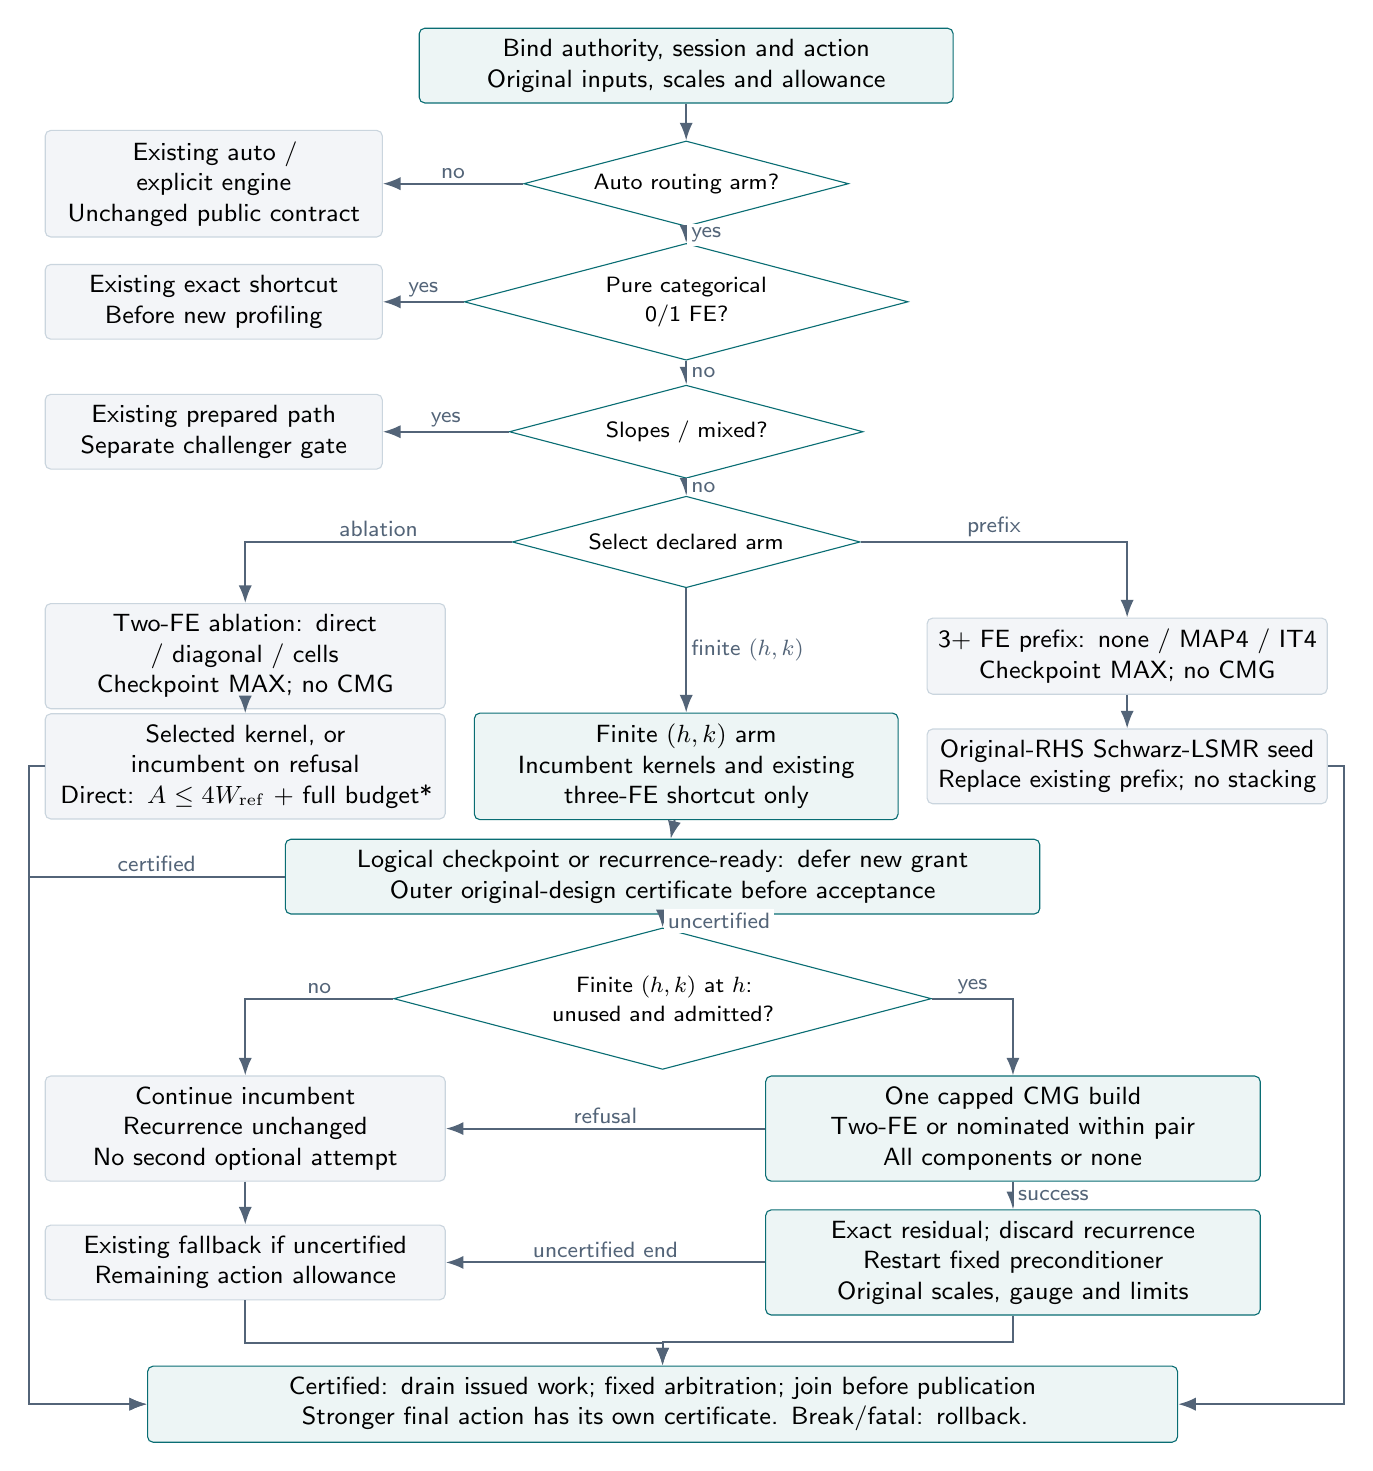
\begin{tikzpicture}[x=1cm,y=1cm,>=Latex,
 box/.style={draw=Rule,fill=Light,rounded corners=2pt,align=center,font=\sffamily\fontsize{9}{11}\selectfont,inner sep=4pt,execute at begin node={\hyphenpenalty=10000\exhyphenpenalty=10000}},
 focus/.style={box,draw=Teal,fill=Pale},
 dec/.style={diamond,draw=Teal,fill=white,aspect=3.8,align=center,font=\sffamily\fontsize{8.5}{10.5}\selectfont,inner sep=2pt,execute at begin node={\hyphenpenalty=10000\exhyphenpenalty=10000}},
 arr/.style={->,line width=0.75pt,draw=Muted},
 lab/.style={font=\sffamily\fontsize{8}{9.5}\selectfont,fill=white,inner sep=1.5pt,text=Muted}]
\node[focus,text width=6.5cm] (start) at (8.4,0) {Bind authority, session and action\\Original inputs, scales and allowance};
\node[dec,text width=2.5cm] (explicit) at (8.4,-1.5) {Auto routing arm?};
\node[box,text width=4.0cm] (exroute) at (2.4,-1.5) {Existing auto / explicit engine\\Unchanged public contract};
\node[dec,text width=2.55cm] (zero) at (8.4,-3.0) {Pure categorical\\0/1 FE?};
\node[box,text width=4.0cm] (exact) at (2.4,-3.0) {Existing exact shortcut\\Before new profiling};
\node[dec,text width=2.75cm] (slope) at (8.4,-4.65) {Slopes / mixed?};
\node[box,text width=4.0cm] (slroute) at (2.4,-4.65) {Existing prepared path\\Separate challenger gate};
\node[dec,text width=3.0cm] (arm) at (8.4,-6.05) {Select declared arm};
\node[box,text width=4.8cm] (ablation) at (2.8,-7.5) {Two-FE ablation: direct / diagonal / cells\\Checkpoint MAX; no CMG};
\node[box,text width=4.8cm] (prefix) at (14.0,-7.5) {3+ FE prefix: none / MAP4 / IT4\\Checkpoint MAX; no CMG};
\node[box,text width=4.8cm] (akernel) at (2.8,-8.9) {Selected kernel, or incumbent on refusal\\Direct: $A\le4W_{\rm ref}$ + full budget*};
\node[box,text width=4.8cm] (pkernel) at (14.0,-8.9) {Original-RHS Schwarz-LSMR seed\\Replace existing prefix; no stacking};
\node[focus,text width=5.1cm] (hk) at (8.4,-8.9) {Finite $(h,k)$ arm\\Incumbent kernels and existing\\three-FE shortcut only};
\node[focus,text width=9.3cm] (inc) at (8.1,-10.3) {Logical checkpoint or recurrence-ready: defer new grant\\Outer original-design certificate before acceptance};
\node[dec,text width=3.95cm] (admit) at (8.1,-11.85) {Finite $(h,k)$ at $h$:\\unused and admitted?};
\node[box,text width=4.8cm] (keep) at (2.8,-13.5) {Continue incumbent\\Recurrence unchanged\\No second optional attempt};
\node[focus,text width=6.0cm] (build) at (12.55,-13.5) {One capped CMG build\\Two-FE or nominated within pair\\All components or none};
\node[focus,text width=6.0cm] (restart) at (12.55,-15.2) {Exact residual; discard recurrence\\Restart fixed preconditioner\\Original scales, gauge and limits};
\node[box,text width=4.8cm] (fallback) at (2.8,-15.2) {Existing fallback if uncertified\\Remaining action allowance};
\node[focus,text width=12.8cm] (terminal) at (8.1,-17.0) {Certified: drain issued work; fixed arbitration; join before publication\\Stronger final action has its own certificate. Break/fatal: rollback.};
\draw[arr] (start.south)--(explicit.north);
\draw[arr] (explicit)--node[lab,above]{no}(exroute);
\draw[arr] (explicit.south)--node[lab,right]{yes}(zero.north);
\draw[arr] (zero)--node[lab,above]{yes}(exact);
\draw[arr] (zero.south)--node[lab,right]{no}(slope.north);
\draw[arr] (slope)--node[lab,above]{yes}(slroute);
\draw[arr] (slope.south)--node[lab,right]{no}(arm.north);
\draw[arr] (arm.west)-|node[lab,near start,above]{ablation}(ablation.north);
\draw[arr] (arm.east)-|node[lab,near start,above]{prefix}(prefix.north);
\draw[arr] (arm.south)--node[lab,right]{finite $(h,k)$}(hk.north);
\draw[arr] (ablation)--(akernel);
\draw[arr] (prefix)--(pkernel);
\draw[arr] (hk)--(inc);
\draw[arr] (akernel.west)--(0.05,-8.9)--(0.05,-17.0)--(terminal.west);
\draw[arr] (pkernel.east)--(16.75,-8.9)--(16.75,-17.0)--(terminal.east);
\draw[arr] (inc.west)--node[lab,above]{certified}(0.05,-10.3)--(0.05,-17.0)--(terminal.west);
\draw[arr] (inc)--node[lab,right]{uncertified}(admit);
\draw[arr] (admit.west)-|node[lab,near start,above]{no}(keep.north);
\draw[arr] (admit.east)-|node[lab,near start,above]{yes}(build.north);
\draw[arr] (build)--node[lab,right]{success}(restart);
\draw[arr] (build.west)--node[lab,above]{refusal}(keep.east);
\draw[arr] (keep)--(fallback);
\draw[arr] (restart.west)--node[lab,above]{uncertified end}(fallback.east);
\draw[arr] (restart.south)--++(0,-0.33)-|(terminal.north);
\draw[arr] (fallback.south)--++(0,-0.54)-|(terminal.north);
\end{tikzpicture}
\end{center}
\vspace{-5pt}
{\smallbody\textbf{Arm guard.} Ablation/prefix arms use \code{checkpoint=MAX}; only finite $(h,k)$ arms reach CMG preparation. Side branches use their own certificate and remaining-allowance fallback. \textbf{*Direct} fully funds certification and may cost more than four iterations on rejection. The intended frontier permits later combinations, but each needs a newly declared complete artifact and qualification; no Cartesian stacking or default promotion is implemented.}


% PAGE 4 ----------------------------------------------------------------------
\newleaf
\sect{03 / INTERNAL CONTRACTS}{Identity, continuation and action limits}
\tagline{Shared by prepared and generic entrypoints; no public report or solver-option redesign.}
{\smallbody
\begin{tabularx}{\linewidth}{P{0.225\linewidth}Y}
\toprule
\textbf{Internal record} & \textbf{Required contents and invariant}\\
\midrule
\code{RoutePlan} & Requested route; supported shape; action accuracy; authoritative factor slots/base flags; global $h$/preset; direct/pair eligibility; nominated pair; worker/memory mode; fixed generation key; optional-attempt state; work reservations. No elapsed-time input.\\
\addlinespace[4pt]
\code{SolveContinuation} & Sample/topology identity, weight generation, coefficient layout, normalization/gauge, RHS identities and order, original RHS scales, current iterate and consumed native iterations. Full recurrence only when explicitly retained and valid.\\
\addlinespace[4pt]
Session preparation state & Immutable session key; frozen $W_0$ and setup cap; spent/issued work; allocation ownership; selected pair/preset; builder cursor; complete reusable hierarchy or parked private preparation. No quota reset on handoff/failure.\\
\addlinespace[4pt]
Action state & Native limit and consumption, selected incumbent's segment counter, active RHSs, original inputs, certificate contract, current recurrence, reserved fallback/output capacity and terminal status.\\
\bottomrule
\end{tabularx}}
\sub{Session identity and reuse}
A projection session fixes sample, weights, basis, accuracy contract and the committed RHS set. Weight identity is a generation, not a pointer. A continuation also binds topology, layout, normalization and RHS order. Reject incompatible reuse before application; unexpected mutation of an immutable in-flight key is an invariant failure.

Completed hierarchies may be reused by a later call with a matching compatible generation key. Partial construction receives no credit for hypothetical future calls. Compatible Low-memory chunks retain session preparation and its single budget, not new build allowances. Do not hide observation-by-RHS copies in a supposedly Low-memory route.
\sub{Native iterations are per action, not a session-wide pool}
\begin{note}
Each OLS action owns its existing native iteration limit. Pilots, restarts, corrections and fallback \emph{within that action} share its remaining allowance. Low-memory chunks retain their existing individual limits and maximum-iteration report aggregation. Never sum all chunks into a new global iteration limit.
\end{note}
The final residual action has its own limit and stronger accuracy contract. PPML \code{iterate()} remains outer IRLS, not a new inner-CMG limit. Work-token accounting is independent of these native counters and may charge all RHS activity even when public iteration reporting uses a maximum.

For two-FE, $h$ counts Diagonal Schur PCG native iterations. For many-FE, it counts the incumbent Schwarz-LSMR segment, not diagonal iterations; any existing qualified MAP prefix still consumes the action allowance. An exhausted action does not gain permission to reach $h$ or to restart.
\sub{Publication and diagnostics}
Preserve public report shapes, requested/used solver semantics and \code{solveroptions}. Mixed Low chunks report the solvers actually used. Do not reinterpret the LSMR-only \code{preconditioner()} option. Add only bounded routing diagnostics: transitions, refusal, representation, preset, reuse, native consumption, work and peak memory. No unbounded event ledger.
\anchor{\code{fe/session.rs} for session reuse; \code{docs/SPEC.md} for public contracts and authoritative semantics.}

% PAGE 5 ----------------------------------------------------------------------
\newleaf
\sect{04 / RESOURCE ADMISSION}{Deterministic work, separate memory}
\sub{Tariffs and the setup envelope}
Use a versioned deterministic tariff for arithmetic, data/record visits, comparisons and moves. Kernels expose checked bounds and bounded precharge. Debit work by bounded chunks, not per-operation atomics; unused reservations may be released only at prescribed boundaries, never to create a timing-dependent route.

Bind $W_0$ to the checked tariff of a \textbf{complete physical incumbent iteration over the initial session batch}, including actual storage work and, for general FE, the Schwarz application. Freeze this deterministic bound once; later deflation or Low chunks do not resize it. It is available before direct preflight and is not elapsed-time measurement. An unavailable or overflowing bound refuses optional work.
\begin{equation*}
 C_{\rm setup}=32W_0,\qquad
 W_{\rm profile}+W_{\rm build}+W_{\rm app\,prep}
 +W_{\rm restart}+W_{\rm cleanup}\le C_{\rm setup}.
\end{equation*}
Profiling, graph aggregation, optional sampling, sorting, hierarchy construction, terminal factors and application preparation are included. Reserve restart and cleanup before any builder grant. Existing Schwarz setup and failed optional work remain charged; this is a late-solve upgrade, not a claim to eliminate incumbent construction cost.
\sub{Admission predicate and application accounting}
Admit only with a valid immutable plan, unused optional opportunity, checked setup capacity, independent peak-memory capacity, remaining native allowance, protected existing fallback/certificate/output reservations, and capacity for at least one candidate update plus certification. Mandatory reserves cannot finance speculative preparation.

Let $B$ be the admitted construction allowance after spent setup work and restart/cleanup reserves. Before chunk $j$, require $\widehat W_j\le B-W_{\rm build,spent}$ and fit within the currently issued grant. Do not start an oversized chunk or overspend before declining. Record and charge later preconditioner applications separately; the setup cap is not permission for unbounded solve work. Native iteration limits remain unchanged. Explicit solvers retain their existing budget semantics.
\sub{Direct admission: comparative work and full funding}
{\smallbody
\textit{Amended after the 14 October GPT Pro review; see page 14.} Price both orientations. Let $A$ include complete candidate-specific work: sunk profiling, assembly, factors, committed solves, reconstruction and any direct-only certificate preparation. Exclude only the structurally shared original-design certificate obligation $C_K$. Define $W_{\rm ref}$ from the incumbent orientation and current committed RHSs at packed width (stride = active width), separately from physical session $W_0$.
\begin{equation*}
 A\le4W_{\rm ref},\qquad
 D_{\rm rem}\le\min(32W_0-S_{\rm opt},U),\qquad M_{\rm peak}\le M_{\rm allowed}.
\end{equation*}
Here $D_{\rm rem}$ funds all remaining work, including $C_K$; $S_{\rm opt}$ is charged optional work and $U$ is spendable work after protected reserves. Every noncertificate prefix obeys the $A$ cap. Never turn certificate allowance into profiling/factor credit or subtract independently computed bounds. Precharge work without double charging sunk profiling. Keep the fallback certificate funded until success.

Choose least work among admitted orientations; tie only by original factor index. No future-RHS or factor-cache credit. A launched finite rejection closes optional routing and preserves the incumbent; fatal errors roll back. Rejected total work can exceed four iterations. This screen makes no runtime claim.
\sub{Peak-memory and reserve implementation}
Include simultaneous incumbent/new states, original inputs, hierarchy/factors, scratch/certificate buffers, stacks, allocator overhead and cleanup. Preallocate fixed service/control/input state before overlap. Later variable numerical payloads are checked, fallible, admitted and gated; small shared-owner controls are admitted/gated but retain Rust's infallible allocation (page 8). Accounting credits are not physical reservations. Hidden unchecked payload growth is ineligible.
}


% PAGE 6 ----------------------------------------------------------------------
\newleaf
\sect{05 / SERIAL CONTROLLER}{Executable transitions and terminal outcomes}
\tagline{Serial is the first implementation to qualify. All guards precede optional work.}
{\smallbody
\begin{tcolorbox}[colback=Light,colframe=Rule,boxrule=0.4pt,arc=0pt,left=5pt,right=8pt,top=7pt,bottom=7pt]
\algline{01}{\textbf{ENTER:} validate authority/support; bind action, session, original inputs/scales/gauge.}
\algline{02}{Explicit/uninjected request: unchanged dispatch. Auto 0/1 categorical FE: exact route.}
\algline{03}{Slopes/mixed: existing path. Otherwise \textbf{SELECT EXACTLY ONE} hidden arm.}
\algline{04}{Ablation: diagonal, cells or direct; \code{checkpoint=MAX}, CMG preparation disabled.}
\algline{05}{Direct alone: test $A$/full funding; solve/certify or retain incumbent; never try CMG.}
\algline{06}{Prefix alone: none/MAP4/IT4 then seeded LSMR; MAX checkpoint, no prefix stacking.}
\algline{07}{Ablation/prefix arms use existing certificate/fallback $\to$ TERMINAL; skip PREPARE.}
\algline{08}{Finite $(h,k)$ only: incumbent $D_f$-PCG, or existing three-FE shortcut/Schwarz-LSMR.}
\algline{09}{\textbf{INCUMBENT:} run existing checkpoints under remaining allowance.}
\algline{10}{Retain the pre-bound physical $W_0$ and all consumed work across chunks.}
\algline{11}{Recurrence-ready: defer grants; require the outer original-design certificate.}
\algline{12}{Finite $(h,k)$ at counter $h$: certify as required before considering a build.}
\algline{13}{No eligible opportunity or failed admission $\to$ INCUMBENT, optional closed.}
\algline{14}{Compatible completed hierarchy $\to$ INSTALL without another build.}
\algline{15}{\textbf{PREPARE:} otherwise mark the session attempt issued; reserve resources.}
\algline{16}{Construct the fixed preset, all nominated replacements or none, under the cap.}
\algline{17}{Refusal $\to$ INCUMBENT, optional closed; retain its untouched recurrence.}
\algline{18}{Fatal: drain/join as prescribed, then atomic rollback. Never retry a preset/pair.}
\algline{19}{\textbf{INSTALL:} validate generation and wrapped-action contract before publication.}
\algline{20}{Recompute original-operator residual; discard incumbent Krylov recurrence.}
\algline{21}{Restart correction with current coefficients and original scales/gauge/recovery.}
\algline{22}{Debit all new updates, certificates and corrections to the same action.}
\algline{23}{Outer-certified: finish. Segment failure: existing fallback, no new candidate.}
\algline{24}{\textbf{FALLBACK:} use remaining action allowance and original input unless a proven}
\algline{}{coefficient-continuation adapter exists. No new quota or native-limit reset.}
\algline{25}{\textbf{TERMINAL:} independent original-problem certificate and joined tasks precede}
\algline{}{commit. Exhaustion without certification returns existing nonconvergence.}
\end{tcolorbox}}
\sub{State machine requirements}
The arm is immutable: ablation/prefix use MAX; finite $(h,k)$ retains incumbents. No direct-to-CMG or new-prefix-to-pair-CMG stack executes. A combination needs a declared complete artifact and qualification. Refusal closes optional selection: no second pair, preset or quota. Retaining an iterate is a \emph{restart}; preserve the incumbent recurrence so refusal resumes it unchanged.

At successful installation the correction interface must implement $r_h=b-Ax_h$, $A\delta=r_h$, $x=x_h+\delta$, with original scales, layout and gauge; for the full design, use its existing weighted least-squares interpretation. A changed preconditioner cannot inherit old LSMR or PCG recurrence scalars. The within branch requires a tested coefficient correction/recovery adapter before it can be enabled.
\sub{Typed results, not a catch-all failure}
Result variants are \code{Certified}, \code{OptionalRefusal}, \code{Nonconverged}, \code{Break} and \code{Fatal}. Optional allocation/quota or declared finite factor/certificate rejection can abstain; panic, invariant breach, invalid input or invalid numerical state are fatal. Do not convert NaNs or corrupted state into a performance fallback.

Use existing fallback support and stronger final-output contracts. A certificate is required for every output action; it does not itself prove forward accuracy, unchanged discrete decisions or inference under near-confounding. Those remain independent verification obligations.

% PAGE 7 ----------------------------------------------------------------------
\newleaf
\sect{06 / NUMERICAL BACKENDS}{Exact two-FE operator; one within-CMG pair}
{\smallbody
\sub{Two-FE Schur path}
With aggregated cell weights $c_{wf}>0$, worker masses $d_w$, firm masses $D_f$, and cross-factor matrix $C$, preserve $S=D_f-C'D_w^{-1}C$, the initial certificate, existing iterative orientation and the exact unsampled outer operator. \textbf{Diagonal Schur PCG uses $D_f$.} True Jacobi and cell-aggregated products are separate numerical/performance qualifications. The stable diagonal identity is
\[
 S_{ff}=\sum_w c_{wf}\,\frac{\sum_{g\ne f}c_{wg}}{d_w}.
\]
Accumulate complementary positive sums after cell aggregation; do not subtract nearly equal masses or use a tiny-value threshold as a new rank rule. Initial CMG uses the existing cutoff-5 predicate: exact low-degree cliques and retained high-degree stars ($k=0$), seed 0. Later sampled trees, if qualified, are fixed with their hierarchy across RHSs/corrections. Connectivity and unbiasedness alone do not establish spectral quality.
\sub{Within nomination and transactional integration}
Add a local backend variant to the existing concrete Schwarz machinery at pinned \code{within} revision \code{297f32d}. Preserve every pair, two-sided partition weights, coordinate wrappers, component grounding/mean projections, elimination/fold/unfold, reductions and small direct components. No slope block is replaced.

For categorical pair $(a,b)$, compute active-size score
\[
 s_{ab}=\max_{c\in\mathrm{components}(a,b)}\min(L_{a,c},L_{b,c}).
\]
Eligibility requires a component above the existing dense threshold. Maximize score; tie by descending sum of retained component dimensions, then ascending original factor indices (bound in the subsequent verification on page 13). These are active sizes, not estimated ranks. Replace all eligible large components of the nominated pair transactionally, or install none, under one allowance. Both large-small blocks remain in a worker-firm-year system. No year-count fence or automatic $q$-core construction is introduced.
\sub{The contract is the fully wrapped local action}
For a sign-transformed local pair, positive active $D$ and fixed symmetric PSD reduced inverse action $B$,
\[
 L=\begin{bmatrix}D&-C\\-C'&E\end{bmatrix},\quad S=E-C'D^{-1}C,\quad
 G=\begin{bmatrix}D^{-1}+D^{-1}CBC'D^{-1}&D^{-1}CB\\BC'D^{-1}&B\end{bmatrix}.
\]
With $T=\left[\begin{smallmatrix}I&D^{-1}C\\0&I\end{smallmatrix}\right]$,
$G=T\,\operatorname{diag}(D^{-1},B)T'$. This gives PSD when $B$ is PSD, but
$\ker G=\{0\}\mathbin{\times}\ker B$, \textbf{not generally the pair-Laplacian kernel}.

Require the fully wrapped inverse action $H_i$ to be fixed, linear, symmetric PSD, exactly preserve the incumbent local kernel, and be positive on the admissible space. Orthogonal projections allow $QGQ$; weighted projections require the correct adjoints/metric, not unexamined repetition of the same wrapper. For unchanged restrictions and two-sided self-adjoint weights,
\[
 P=\sum_i R_i'\Omega_i H_i\Omega_iR_i,\qquad
 \ker P=\bigcap_i\{x:\Omega_iR_ix\in\ker H_i\}.
\]
The identity follows from nonnegative local quadratic forms. It preserves the assembled kernel, not global Gram nonsingularity. Match the modified-LSMR inner product and retain its one assembled inverse-Gram action per iteration.

Prove cycle positivity from smoothing, adjoint transfers and the coarse solver; numerical linearity/symmetry/positivity/nullspace witnesses supplement that proof. Fixed symmetric cycles from zero may qualify. Tolerance-stopped inner CG and fixed-count ordinary CG are not fixed linear preconditioners. A retained-star full-pair cycle needs a correctly dimensioned backend with adjoint embedding/restriction, never a fictitious reduced dimension.
}
\anchor{\code{cmg\_schur.rs}, \code{cmg\_schur/sampling.rs}; reviewed \code{within 297f32d} pair/block-elimination baseline.}

% PAGE 8 ----------------------------------------------------------------------
\newleaf
\sect{07 / UPSTREAM CONCURRENCY}{A controlled builder, not racing cancellation}
\tagline{Current-artifact mapped concurrency witnesses pass; performance qualification remains pending.}
{\smallbody
\sub{Required CMG construction interface}
The serial builder exposes \code{grant}, \code{park}, \code{drain\_issued\_prefix}, \code{abandon\_unissued\_suffix} and \code{fatal}. Stable control sites cover assembly, sorting, hierarchy, terminal factors and application preparation. Primitive chunks cost at most 1024 tariff units; allocations and faults have separate gates. Split or park before a chunk that does not fit: a chunk bound never permits grant overshoot. The unlimited controller preserves explicit construction and budget semantics.
\sub{Eligibility and worker ownership}
Promotion requires serial qualification first. Overlap requires $P\ge2$, $4<h<\infty$, bounded kernels and joint memory admission. After four \emph{incumbent} iterations, exclusively lease one existing executor worker; cap foreground work at $P-1$ with a fixed partition and reductions. The coordinator must not consume an additional blocked slot or help-run the parked builder. No nested pool, capacity-dependent nested waits or barriers including nonparticipants.

The session owns service state, input copies and lease across compatible Low chunks; value leases allocate nothing. A parked builder never borrows reused chunk scratch. Refresh authoritative parent memory/budget for each wider RHS block before further allocation; initial $W_0$, $B$ and $G$ never reset. Early completion does not release the worker. Drain/join before inputs or publication escape; parking is not joining. SPI stays on the main thread.
\sub{Allocation amendment and its limits}
Establish fixed service, synchronization, input and cleanup state before launch. Fixed input copies are checked/fallible under aggregate admission; no per-copy injected gate is required. Full eventual hierarchy preallocation is not required. Later variable numerical payloads are checked, fallible, admitted and gated at stable sites with deterministic sizes/order/lifetimes. Small shared-owner headers are admitted and gated, but stable Rust \code{Arc::new} remains infallible. Protect solve, certificate and shutdown capacity; prohibit hidden unchecked payload growth and track partial initialization.

Optional refusal is transactional. Cleanup transport is nonallocating; existing error \code{String} construction and diagnostics can allocate. Credits are not physical reservations. Successful runs assume the same allocation outcomes; fixed logical-site injections must repeat routes, status and accounting under scheduling changes. Exogenous allocation failure can change outcomes; allocator abort and process death are outside the survival guarantee. Repeatability is conditional, and logical work bounds do not guarantee allocator or cancellation wall time.
\sub{Grant and ownership protocol}
One owner grants prepaid deterministic prefixes: each eligible four-iteration epoch adds $W_0$, capped by admitted $B$ after restart/cleanup reserves. Grants and spending persist across Low chunks. Recurrence-ready or batch-end defers grants until the outer original-design certificate decides. Failure at iteration 4 or $h$ services that same frozen optional checkpoint before correction advances; allowance never renews. At uncertified $h$, grant remaining $B$ and join. Install only at the declared exact-residual restart.
\sub{Failure ordering and deterministic termination}
Drain to the issued frontier or intrinsic completion/refusal/fatal event. Precedence is \textbf{Break; fatal errors in fixed kind/task order; independently certified success; optional refusal}. Task 0 is foreground, task 1 preparation; logical failure sites are stable. Except for Break, local failure cannot truncate prescribed peer work by arrival time. Abandon only unissued work; join before publication/rollback and release capacity only at the declared boundary. A stronger final action needs its own certificate.
\anchor{Codex amendment informed by an actual generic GPT Pro review, 14 October 2026, 5m48s, in the \href{https://chatgpt.com/c/6aceddfe-edec-83ea-a216-6d1fbf408136?temporary-chat=true}{retained review conversation}. No project code or results were submitted for that review; it is not exact-project approval.}
}

% PAGE 9 ----------------------------------------------------------------------
\newleaf
\sect{08 / PARALLEL GRANT TIMELINE}{Fixed checkpoints, cumulative issued work}
\tagline{Illustration: $h=16$, $B=10W_0$. Values illustrate the protocol, not an additional policy constant.}
\begin{center}
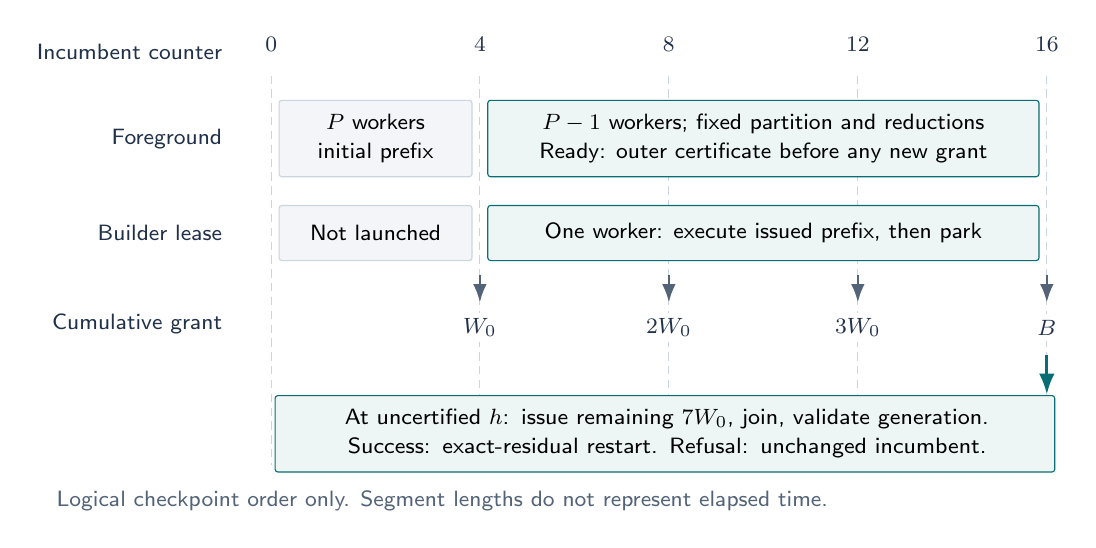
\begin{tikzpicture}[x=1cm,y=1cm,>=Latex,
 lab/.style={font=\sffamily\fontsize{8.5}{10.5}\selectfont,align=center,text=Ink},
 tile/.style={draw=Rule,fill=Light,rounded corners=1pt,align=center,font=\sffamily\fontsize{8.5}{10.5}\selectfont,inner sep=5pt},
 line/.style={draw=Muted,line width=0.8pt}]
\node[lab,anchor=east] at (2.5,0.05) {Incumbent counter};
\foreach \x/\t in {3.0/0,5.65/4,8.05/8,10.45/12,12.85/16} {
 \draw[draw=Rule,densely dashed] (\x,-0.25)--(\x,-5.2);
 \node[lab] at (\x,0.15) {$\t$};
}
\node[lab,anchor=east] at (2.5,-1.05) {Foreground};
\node[tile,minimum width=2.45cm,minimum height=0.85cm] at (4.325,-1.05) {$P$ workers\\initial prefix};
\node[tile,fill=Pale,draw=Teal,minimum width=7.0cm,minimum height=0.85cm] at (9.25,-1.05) {$P-1$ workers; fixed partition and reductions\\Ready: outer certificate before any new grant};
\node[lab,anchor=east] at (2.5,-2.25) {Builder lease};
\node[tile,minimum width=2.45cm,minimum height=0.7cm] at (4.325,-2.25) {Not launched};
\node[tile,fill=Pale,draw=Teal,minimum width=7.0cm,minimum height=0.7cm] at (9.25,-2.25) {One worker: execute issued prefix, then park};
\node[lab,anchor=east] at (2.5,-3.4) {Cumulative grant};
\foreach \x/\t in {5.65/{W_0},8.05/{2W_0},10.45/{3W_0},12.85/{B}} {
 \draw[-{Latex},line] (\x,-2.78)--(\x,-3.13);
 \node[lab,fill=white,inner sep=2pt] at (\x,-3.45) {$\t$};
}
\draw[-{Latex},draw=Teal,line width=1pt] (12.85,-3.8)--(12.85,-4.3);
\node[tile,fill=Pale,draw=Teal,text width=9.55cm] at (8.0,-4.8) {At uncertified $h$: issue remaining $7W_0$, join, validate generation.\\Success: exact-residual restart. Refusal: unchanged incumbent.};
\node[lab,anchor=west,text=Muted] at (0.15,-5.65) {Logical checkpoint order only. Segment lengths do not represent elapsed time.};
\end{tikzpicture}
\end{center}
\vspace{-4pt}
\sub{Executable grant rule}
{\smallbody
\begin{tcolorbox}[colback=Light,colframe=Rule,boxrule=0.4pt,arc=0pt,left=8pt,right=8pt,top=6pt,bottom=6pt]
Initialize $G=0$ once per compatible session, not on Low-chunk handoff.\\
At each eligible four-iteration epoch before $h$:\quad $G\leftarrow\min(B,G+W_0)$.\\
At $h$, provided the action is not already certified:\quad $G\leftarrow B$.\\
Builder executes only a deterministic prefix authorized by $G$, then parks.\\
Recurrence-ready: defer grant; require the outer original-design certificate.\\
Rejection at 4 or $h$: service the frozen checkpoint before correction advances.\\
$G$ and setup spending persist across compatible Low-memory chunks; no refill.
\end{tcolorbox}}
\sub{Terminal examples and Low-memory handling}
{\smallbody
\begin{tabularx}{\linewidth}{P{0.29\linewidth}Y}
\toprule
\textbf{Foreground event} & \textbf{Required builder and controller behavior}\\
\midrule
Ready at iteration 10 & Grant stays $2W_0$ until the outer certificate decides. On success, drain that prefix and arbitrate before accepting. Failure follows the declared continuation.\\
\addlinespace[3pt]
Early or late builder & An early result cannot switch the solver or return its worker. A late builder is joined at the same frozen checkpoint; no readiness-based routing.\\
\addlinespace[3pt]
Compatible Low chunk finishes & Outer-certify and drain issued work. The session service retains private preparation, exclusive lease and ledger for compatible chunks. No quota reset or merged native limit.\\
\addlinespace[3pt]
Committed RHS set finishes & Drain/arbitrate, abandon only unissued work, terminate and join before publication. A stronger final action retains its own certificate obligation.\\
\addlinespace[3pt]
Break, fatal, refusal & Break cancels; fatal outranks success; optional refusal does not. A failure's arrival time cannot decide how much prescribed peer work executes.\\
\bottomrule
\end{tabularx}}
\vfill
{\smallbody\textbf{Boundary rule.} Recurrence readiness is not certification. Process the original-design certificate before a coincident grant, including at $h$. Parking retains ownership; only the declared boundary returns capacity. Fresh current-artifact overlap witnesses pass; performance qualification remains pending.}

% PAGE 10 ---------------------------------------------------------------------
\newleaf
\sect{09 / DELIVERY PROGRAM}{Independent stages, unchanged model semantics}
{\smallbody
\begin{tabularx}{\linewidth}{P{0.075\linewidth}P{0.285\linewidth}Y}
\toprule
\textbf{Stage} & \textbf{Implementation deliverable} & \textbf{Required boundary before promotion}\\
\midrule
0 & Shared controller, accounting, continuation and capped serial CMG & Prepared/generic entrypoints agree. Unlimited builder matches current construction. Lock immutable starting baseline and stage incumbent.\\
\addlinespace[3pt]
1 & Serial two-FE routing & Initial retained-star preset, four finite $h$ candidates, exact residual restart, independent science and resource tests.\\
\addlinespace[3pt]
2 & True diagonal, cell products and direct components & Qualify each independently; no assumption that a mathematically exact identity is bitwise or performance equivalent.\\
\addlinespace[3pt]
3 & Within-CMG backend, correction adapter and prefix experiments & Prove wrapped-action contract. Retain other pair blocks. Qualify coefficient IT and prefix policy separately, without a Cartesian search.\\
\addlinespace[3pt]
4 & Sampling, then binary overlap & Sampling witnesses precede $k=1,2$ comparisons. Freeze $h$/preset before serial-versus-overlap gate. Serial wins by default on failure.\\
\addlinespace[3pt]
5 & PPML integration & Separate accepted/speculative lifecycle, weight-generation and outer-iteration qualification. OLS success authorizes no PPML promotion.\\
\bottomrule
\end{tabularx}}
\sub{General categorical prefix and prepared slopes}
Ordinary auto retains its existing at-most-four-MAP-sweep three-FE shortcut. Three hidden arms implement no prefix, at most four MAP sweeps, or four compact IT cycles (at most eight native sweeps). They replace, never stack with, the existing shortcut. Uncertified coefficients warm-start LSMR from untouched original RHSs through a fresh original-design residual. Outer prefix certification uses the requested model tolerance. Every sweep consumes the action allowance; admission includes seed/handoff memory. No prefix is promoted.

Prepared slopes and mixed systems keep their current supported path until an independently qualified LSMR/IT challenger exists. Do not describe that path as uniformly LSMR. Include efficient coefficient IT and standalone diagonal-versus-Schwarz arms in eligible comparisons, not in an uncontrolled automatic solver tournament.
\sub{PPML: structural sharing first, numerical ownership unchanged}
The off-by-default PPML source stage shares component topology/indexing only. Preserve canonical outer engines, accepted/pending frame ownership, strict checkpoints, support handling, Low-memory restrictions and outer-iterate semantics. Current weighted masses, trees, factors and hierarchies are rebuilt for each applicable numerical generation. Support changes invalidate affected topology and numerical keys.

Commit pending component indices only when their generation is accepted; rejection discards pending state without replacing accepted topology. Numerical data always belong to current weights. Old factors are not current inverses. No OLS result qualifies PPML, and this structural stage does not authorize new per-IRLS solver selection.

Qualify weight/support transitions, separation, both bias modes, final outputs and outer iteration behavior independently. Saved effects, coefficient/gauge recovery, inference and all protected discrete decisions must remain consistent with existing authority.
\sub{Repository and release governance}
Pin upstream revisions and record the precise CMG and within patches. Apply the user-approved controlled measurement rules on pages 11 and 22. Any exception to the max(5\%, 1 ms) current-auto gate or scientific semantics requires a user decision, not a new local fence or relaxed rule.


% PAGE 11 ---------------------------------------------------------------------
\newleaf
\begin{compactleaf}\smallbody
\sect{10 / PERFORMANCE QUALIFICATION}{Finite selection, paired uncertainty, one holdout}
\sub{Arm manifest and timing scope}
Predeclare eligible arms by support and output/accuracy contract, cells, seeds, workers, failures/timeouts, order, analysis unit and finite budgets. Measure complete calls, including construction, outputs and actual compatible reuse. The approved controlled protocol below supersedes the original bootstrap selection plan; historical observations retain their original analysis.

Initially compare four finite $h$ policies with retained stars plus unchanged baseline. After sampling qualification, allow at most $4\times3=12$ $(h,k)$ policies plus baseline. These implemented policies retain incumbent kernels and the existing three-FE shortcut; ablation and prefix arms are separate. A future combination needs a newly declared complete artifact and qualification. No Cartesian search across kernels, prefixes, presets and overlap; retain baseline measurements throughout.
\sub{Isolated SCC A, controlled Mac B, untouched Mac C}
{\smallbody
\begin{tabularx}{\linewidth}{P{0.16\linewidth}P{0.19\linewidth}Y}
\toprule
\textbf{Partition} & \textbf{Run design} & \textbf{Selection or decision rule}\\
\midrule
A: SCC discovery & 3 rounds $\times$ 3 measured repetitions; 1 warmup/round & Verified same-node isolation. Point estimates shortlist at most four by baseline violations, worst normalized regret, geometric-mean baseline ratio, then conservative ties. Nine slots are not asserted independent.\\
\addlinespace[4pt]
B: Mac selection & 12 mirrored multiarm rounds & Two calls/distinct arm: a frozen permutation and its reverse, shared across comparisons. Among gate passers minimize worst normalized internal upper bound. Ties prefer baseline, retained stars, larger $h$, fewer trees.\\
\addlinespace[4pt]
C: Mac holdout & 24 ordinary two-arm ABBA/BAAB blocks per required edge & One frozen public artifact; no cross-edge call reuse. Failure or uncertainty retains the incumbent. No runner-up, retuning or development use of C. Freeze this schedule before Mac B; page 17 governs activation.\\
\bottomrule
\end{tabularx}}
\sub{Acceptance margins and statistical interpretation}
For each required comparison, let $B,N$ be within-block geometric-mean reference/candidate times. Test median excess $E=N-B-\max(\epsilon B,0.001)$ seconds: $\epsilon=.05$ for original-baseline and selected-incumbent protection; $.20$ for internal frontier comparisons. Preserve every eligible declared comparison and the absolute 1 ms branch; do not select a noisy fastest observed arm.

Use an attainable one-sided order-statistic bound, $\alpha=1/40$. For $X\sim\mathrm{Binomial}(n,.5)$, choose the smallest $k$ with $\Pr(X\ge k)\le\alpha$; set $U=E_{(k)}$. Pass if $U\le0$; no attainable rank is inconclusive. Coverage assumes independent blocks with a common median; it is not simultaneous. Preserve shared-reference correlations; report ratios separately. Page 22 states the A/A limitation.

Retain failures and timeouts as failures; do not drop them or resample until passing. Report family/cell tails, worst regret and uncertainty alongside geometric means. An inconclusive upper-bound gate does not pass. Baseline retention neither proves the internal target nor establishes universal performance safety.
\sub{External comparisons and release measurements}
Compare fixest, reghdfe and ppmlhdfe only on eligible accuracy-matched, complete end-to-end tasks including required outputs. Keep default and matched-strict comparisons separate. Do not infer a win from differing tolerances, missing saved effects or omitted final inference work.

Use controlled paired Mac timing after stable edits/profiling. Record OS bursts; invalidate complete blocks for known competing compute only under frozen external-evidence rules and bounded attempts. No quiet-desktop gate applies. Freeze C before B; no opportunistic extension. Protect both baselines, bind policy/seed/revision, and require fresh untouched validation for later stages.
\end{compactleaf}

% PAGE 12 ---------------------------------------------------------------------
\newleaf
\sect{11 / VERIFICATION AND RELEASE}{Evidence required before an automatic route ships}
{\smallbody
\begin{tabularx}{\linewidth}{P{0.22\linewidth}Y}
\toprule
\textbf{Verification area} & \textbf{Minimum evidence and adversarial cases}\\
\midrule
Numerical kernels & Independent dense/high-precision witnesses; exact-operator adjoints; local linearity, symmetry, positivity and nullspace; stable Schur diagonal; retained-star dimensions and adjoint wrappers. Numerical witnesses supplement proofs.\\
\addlinespace[3pt]
Scientific outputs & 0/1/2/3/4/8/many FE; tiny retained/dense/weak/real AKM; repeated cells, skewed weights, disconnected and near-confounded third FE; slopes, multi-RHS/inactive RHS, Low, saved-FE gauge, strict final residuals, coefficients and inference.\\
\addlinespace[3pt]
Controller and resources & Exact-residual/original-scale restart; unchanged incumbent on refusal; per-action limits and Low maximum aggregation; shared setup cap; no second candidate; peak-memory and checked-bound exhaustion; full mapped/replay transaction checks.\\
\addlinespace[3pt]
Parallel ownership & Two workers and larger budgets; early/late/parked builders; certificates around $h$; grants, allocation faults, deterministic fault ordering, Break, panic and rollback. Fixed-mode/$P$/seed bitwise output and route repeats under schedule perturbation; cross-worker science/discrete agreement.\\
\addlinespace[3pt]
PPML separately & Accepted/speculative cache publication, rejection rollback, weight/support transitions, separation, both bias modes, strict checkpoints, final outputs and outer-iteration semantics.\\
\bottomrule
\end{tabularx}}
\sub{Explicit implementation bindings, not hidden policy changes}
{\smallbody
\begin{tabularx}{\linewidth}{P{0.105\linewidth}Y}
\toprule
\textbf{Binding} & \textbf{Freeze before enabling the affected stage}\\
\midrule
B1 & Versioned tariff, primitive bounds, reserve computation, native-counter debit mapping and exact checkpoint mapping. Preserve established action/Low semantics.\\
B2 & Preserve the pair's primary score; secondary tie is descending total retained component dimension, then ascending original factor indices.\\
B3 & Fixed fatal kind/task ordering, logical fault locations and resumable Low epoch mapping. Cumulative grants must never reset or depend on readiness.\\
B4 & Bind the controlled block estimand, conditional order-statistic bounds, ranking rule and frozen C schedule (pages 11 and 22). The original paired-bootstrap binding below is historical and superseded.\\
\bottomrule
\end{tabularx}}\par\vspace{5pt}
This checklist records specification bindings. Page 13 identifies source bindings; page 15 separates integrated checks from pending performance qualification. Record bindings in code/tests and the qualification manifest, not a data-dependent classifier. Implementation and native checks alone do not promote an optional branch.
\sub{Readiness record and source anchors}
Before promotion, require implementation/revision pins; numerical-contract proof and witnesses; action/resource/rollback tests; supported-output compatibility; passing A/B selection; a frozen complete policy; and passing untouched C. Otherwise the optional feature remains off. The specification is not a promotion receipt; outcomes and the current method are on pages 18--22.

{\tinybody
\textbf{Repository authority:} \code{docs/SPEC.md}.\quad
\textbf{Two-FE workspace:} \code{crates/fereg-core/src/fe/borrowed\_map.rs}.\par
\textbf{Exact operator / sampling:} \code{cmg\_schur.rs} and \code{cmg\_schur/sampling.rs} within the FE module.\par
\textbf{Reuse:} \code{fe/session.rs}.\quad
\textbf{Direct mathematics:} \code{ols/canonical\_products.rs}; reuse kernels, not estimator lifecycle or rank authority.\par
\textbf{Upstream baseline:} pinned \code{within 297f32d}, as reviewed in the approved plan; retain pair coverage, partition weights and block-elimination wrappers. These are implementation anchors, not a claim of fresh repository inspection.}
\vfill
{\sffamily\bfseries\fontsize{9.5}{12}\selectfont\color{Teal}RELEASE STATUS: REVIEWED SPECIFICATION. PERFORMANCE QUALIFICATION PENDING.}

% PAGE 13 ---------------------------------------------------------------------
% Subsequent verification authored by Codex, not by GPT Pro.
\newleaf
\begin{compactleaf}
\sect{12 / SUBSEQUENT CODE VERIFICATION}{Integrated experiments; promotion pending}
\tagline{Implementation note authored by Codex after the original GPT Pro specification.}
\begin{note}\smallbody
The explicit OLS CMG repair artifact \code{72ff85} passes focused checks, independent source reviews, the full suite and universal build, plus 1,139 fresh native calls, eight Stata fixtures and five Break checks. The dynamic-weight prerequisite passes unchanged. Repaired ablation and policy A prerequisites are complete (page 15). Performance remains unqualified; ordinary \code{auto} and explicit IT stay unchanged.
\end{note}
{\smallbody
\begin{tabularx}{\linewidth}{P{0.075\linewidth}Y}
\toprule
\textbf{Binding} & \textbf{Current implementation and remaining boundary}\\
\midrule
B1 & Checked tariffs, accounting and checkpoints are bound in the controller sources below: $h\in\{4,8,16,32\}$, $32W_0$ setup and $4W_0$ restart reserve. General-FE work includes incumbent Schwarz and checked replacement startup. Per-action iteration limits, Low-chunk maximum reporting and the separate final action remain distinct from setup accounting.\\
\addlinespace[4pt]
B2 & Preserve primary score $\max_c\min(L_{a,c},L_{b,c})$. Tie by \emph{descending sum of retained component dimensions}, then ascending original factor indices. Total local dimension is not used. This binds the reviewed keys.\\
\addlinespace[4pt]
B3 & Experimental overlap uses an exclusive existing-worker lease and session service across compatible Low chunks. Grants, deferred certification, fixed fatal ordering and gated allocation follow pages 8--9. Fresh current-artifact native/Break checks pass; performance remains separate.\\
\addlinespace[4pt]
B4 & \textbf{Historical binding, superseded by pages 11 and 22.} \code{bench/routing.py} used disjoint hashed A/B/C inputs, one warmup and 3/7/7 paired repetitions; paired-median bootstrap with 10,000 draws, seed 739391 and nominal 95\% intervals. A used medians; B/C used upper endpoints. Prior results keep that analysis.\\
\bottomrule
\end{tabularx}}
\sub{Kernel distinctions preserved in the candidate}
{\smallbody
The \code{cells} arm changes the Schur product representation while retaining the incumbent $D_f$ preconditioner. The \code{diagonal} arm tests the true Schur diagonal separately. These are distinct experiments, not an implicit combined substitution.

Direct follows pages 5 and 14: $A\le4W_{\rm ref}$ at packed width, full funding and peak-memory admission. No factor-reuse cache exists. Rejection closes optional routing and can exceed four iterations total. Core, dense-QR and four fresh current-artifact native cases pass; these scientific checks establish no performance claim.

Ordinary explicit IT retains observation-space acceleration. Hidden \code{inject=it\_coefficients} tests the coefficient-space Euclidean metric, selected by complete simultaneous-memory comparison (ties favor coefficient space). Its trajectory changes; original-weight certification, rejection safeguards and factor-slot recovery remain required. Page 15 records the failed qualification and separate prefix arms.
}
\sub{Historical statistic and source anchors}
{\smallbody
For ratio statistic $q$, normalized excess regret is
\[
 g=\frac{q-1}{\max\!\left(\epsilon,\,0.001/\operatorname{median}(t_{\rm reference})\right)},
 \qquad \epsilon=0.05\ \text{for protection},\quad 0.20\ \text{for internal arms}.
\]
The historical gate was $g\le1$; it is not current acceptance. Pages 11 and 22 specify controlled excess-score bounds. Prior bootstrap outcomes on pages 18--21 remain unchanged.
}
\anchor{FE paths below \code{crates/fereg-core/src/}.\par
Controller: \code{fe/routing.rs}, \code{fe/borrowed\_map.rs}, \code{fe/borrowed\_map/routing\_lsmr.rs}.\par
Kernels: \code{fe/routing\_direct.rs}, \code{fe/routing\_overlap.rs}, \code{fe/borrowed\_map/irons\_tuck.rs}.\par
Selection: \code{bench/routing.py}; bootstrap: \code{bench/time\_exact.py}.}
{\tinybody Published main pins: \href{https://github.com/johannes-schmieder/within/commit/efe35ee386ad989b043a5076d01d879ca410ff19}{\code{within/schwarz efe35ee}}; \href{https://github.com/johannes-schmieder/CMG/commit/b989eddfc3bf7ad130c76df8d0cceaf9801e1d72}{\code{CMG b989edd}}. No pending upstream branch decision. Prior serial evidence uses earlier pins (page 15).}
\vfill
{\sffamily\bfseries\fontsize{9.5}{12}\selectfont\color{Teal}DEFAULT AUTO UNCHANGED. FINITE PERFORMANCE QUALIFICATION PENDING.}
\end{compactleaf}

% PAGE 14 ---------------------------------------------------------------------
% Codex policy amendment informed by actual GPT Pro review, not new Pro authorship.
\newleaf
\sect{13 / REVIEWED ACCOUNTING AMENDMENT}{Compare like work; fund the whole attempt}
\tagline{Codex amendment, adopted after an actual GPT Pro review on 14 October 2026.}
\begin{note}\smallbody
\textbf{Review provenance.} GPT Pro reviewed the exact tariff flaw and proposed correction in the retained \href{https://chatgpt.com/c/6aceddfe-edec-83ea-a216-6d1fbf408136?temporary-chat=true}{routing review conversation}. Its conclusion was: ``Approve symbolic exclusion of a common certificate obligation---not numerical credit from an adjustable certificate bound.'' This page is Codex's implementation-facing amendment, not newly Pro-authored text.
\end{note}
\sub{Why the original gate was rejected}
{\smallbody
The original $A+C\le4W_0$ compared a complete direct action against iterations that excluded the same final certificate. For the reviewed bounds, write $n\ge p\ge q\ge1$ for rows and incumbent eliminated/retained levels, $r\ge1$ for active RHSs, and $b=\lceil n/512\rceil$. With full-width storage, GPT Pro verified
\[
\begin{aligned}
C-4W_0={}&(112r+72)(n-p)+(220r+40)(p-q)\\
&+(80r-8)(q-1)+64r(b-1)+16(r-1)+8\ge8.
\end{aligned}
\]
Thus the old gate cannot admit any positive direct construction cost. An inactive-stride witness does not repair that defect. No empirical multiplier increase is authorized.
}
\sub{Exact replacement and nonfungible certificate reservation}
{\smallbody
$W_{\rm ref}$ is the packed current-action reference in the incumbent orientation. It uses only committed RHSs and their fixed partition. Physical storage operations remain fully charged; later Low chunks never reset physical session $W_0$ or its $32W_0$ envelope.

Define $A$ by disjoint operations outside a verified shared certificate kernel $K$. Include both-orientation profiling and all direct-only work. In the candidate, $K$ uses the original design, validated original weights, retained reference norms, tolerance and common \code{certify} kernel. Its bound includes fresh candidate residual norms, the shifted compensated pass and scaled fallback. Direct-only coefficient validation and scratch/layout preparation, $2(p+q)r+128$ units, stay in $A$. Equal tolerances alone do not establish commonality; disputed work stays candidate-side.
\[
\boxed{A\le4W_{\rm ref}}\qquad
\boxed{D_{\rm rem}\le\min(32W_0-S_{\rm opt},U)}
\]
The full attempt includes $C_K$ and simultaneous-memory admission. Every profiling/census/assembly prefix obeys the first cap; the complete remaining bound obeys the second. Increasing $C_K$ can only tighten resource admission. It cannot enlarge the first cap. Charge before execution, retain spent work on rejection, and never double charge sunk work.

Keep incumbent recovery and its certificate independently funded until direct succeeds: rejection can require two certificates. A stronger final action is a separate obligation unless actually discharged. Respect the certificate's final outcome, including any scaled fallback. Finite refusal returns to the untouched incumbent with no second optional candidate. Break, panic and invalid numerical state retain fatal rollback.
}
\sub{Verification boundary}
{\smallbody
Admission needs an independent phase-by-phase envelope checked against executed kernels and full-width production. Required witnesses include unequal weights, repeated cells, refusal, boundaries, overflow, certificate branches, padding invariance, Low persistence, fallback and rollback; numerical oracles cover projections, coefficients, saved gauge, inference and protected decisions.

\textbf{Source, core and fresh integrated native witnesses pass.} Core tests, dense-QR checks and four current-artifact native cases cover unit/unequal weights, Fast/Low, workers 1/4, saved gauge and inference. Fast admission certifies 65 active RHSs. Source review confirms prefix/full gates, packed reference, rejection charge and the shared certificate. Performance qualification remains pending.

Different residuals can take different certificate branches. This policy proves neither equal actual costs nor four-iteration competitiveness; rejected total work may exceed four iterations. No speedup, tournament pass, default promotion or completed PPML qualification is asserted.
}
% PAGE 15 ---------------------------------------------------------------------
% Current evidence and implementation boundaries authored by Codex.
\newleaf
\begin{compactleaf}
\renewcommand{\smallbody}{\fontsize{9.2}{10.5}\selectfont\color{Ink}\RaggedRight}
\sect{14 / EVIDENCE AND EXPERIMENTAL BOUNDARIES}{Implemented scope and evidence}
\tagline{Codex verification note. All results remain bound to their tested artifacts and declared scope.}
\sub{Current mapped verification; performance remains open}
{\smallbody
Repaired plugin \code{72ff85} passes 239 Python tests (13 skips), 1,331 core tests (three declared exclusions), 195 plugin tests and ten isolated allocator audits, oracles, strict Clippy, fuzz, ABI and universal Mac build. Its 1,139 fresh native calls pass: 68 ordinary cases retain exact parent comparisons; five typed OLS CMG cases pass independent science, exact fixed-worker repeats and 2/4/8/16-worker science/discrete checks. Supplemental routing/IT, direct, overlap and PPML topology panels pass, as do eight Stata fixtures and five Break checks. Builder checks at 2/4 workers each repeat twice after actual work, with rollback/reset.

The wider-Low-block envelope repair passed independent review. The first Low-install expectation failed correctly: sort/load work exceeded the cap. Separate refusal and two genuine Low-install witnesses pass. The first builder fixture failed with long-macro r(198); indexed locals repaired the harness. Both failures remain recorded; witness fixes changed no runtime.

New wide-129/one-worker profiles preserve science: dense-meat samples 119/116, finite moments 84/83, Schur 26/24 (candidate/baseline). They prove no speedup or nonregression. The optional CMG CPU sampler's sandbox attach failed (255); preserve it without retry or cost claim. Candidate science passed.

Repaired ablation completes 26 wrappers: 320 initial passes and 320 passing repeats. Policy A completes 42: 846 initial passes and 846 passing repeats. Each retains 18 optional MAP/IT/compact-IT unavailabilities on weak/high-degree-weak/dynamic-weight cells at workers 1/4; zero science blocks remain. Original policy A's 844 passes and two IT slope-warning checker blocks stay recorded. The reviewed, source-derived warning correction passes 58 focused tests and six fresh baseline/IT control/repeat calls at workers 1/4, exactly matching old failed-call outputs. Provenance is published; runtime, numerical scope and tolerances are unchanged. These are untimed prerequisites; later timings appear on pages 18--20.
}
\sub{Explicit compact IT: failed qualification is preserved}
{\smallbody
The original 38-cell all-success protocol on prior serial artifact \code{a00a78f1} failed after 16 passing comparisons: old IT exhausted its iteration limit on a one-worker weak graph before candidate dispatch. A separate bounded, untimed completion obtained all 38 cells, reusing the 16 verified comparisons and retaining that failure.

Both versions pass 32 cells with independent truth, two exact repeats, scoped compatibility and cross-worker checks. The same six cells are unsuccessful, but failure modes are not identical:\par
\begin{tabularx}{\linewidth}{P{0.225\linewidth}Y Y}
\toprule
\textbf{Family} & \textbf{One worker: old / candidate} & \textbf{Four workers: old / candidate}\\
\midrule
Weak & iteration exhaustion / exhaustion & iteration exhaustion / exhaustion\\
High-degree weak & 120 s timeout / timeout & 120 s timeout / timeout\\
Dynamic weights & iteration exhaustion / 120 s timeout & iteration exhaustion / exhaustion\\
\bottomrule
\end{tabularx}
The completion is not a replacement qualification pass, performance result or candidate-wide scientific acceptance. Ordinary explicit IT therefore retains its incumbent implementation. Compact IT remains the hidden \code{inject=it\_coefficients} challenger; no weak family or unsuccessful observation is removed.
}
\sub{New source stages remain experimental}
{\smallbody
\begin{tabularx}{\linewidth}{P{0.20\linewidth}Y}
\toprule
\textbf{Stage} & \textbf{Implemented scope; qualification boundary}\\
\midrule
Parallel CMG & Existing-worker lease, cumulative grants and Low session ownership; outer certificate before grants; fixed arbitration. Fresh install/refusal/Break witnesses pass; performance gate pending.\\
Categorical prefixes & Hidden none / four MAP / four compact IT cycles (at most eight sweeps), replacing one shortcut. Original-RHS warm start, model-tolerance certificate and full handoff accounting. No promotion.\\
PPML topology & Off-by-default component-index sharing, accepted/pending generations and current-weight rebuild. Fresh native topology checks pass; repair preserves PPML arithmetic. No promotion.\\
\bottomrule
\end{tabularx}
}
\anchor{Current plugin SHA-256:\par \code{72ff85cc33e088ec85c9e30feddc589a3f2aa1068bca1d812e74fba498c3207e}.\par Native transcript: \code{3eb756e3}; full identities and preserved failures: \code{docs/VALIDATION.md}.\par Contracts: \code{fe/routing\_overlap.rs}, \code{fe/borrowed\_map/categorical\_prefix.rs}, \code{fe/session.rs}.}
\vfill
{\sffamily\bfseries\fontsize{9.5}{12}\selectfont\color{Teal}NO DEFAULT PROMOTION. NO PERFORMANCE CLAIM. FINITE QUALIFICATION PENDING.}
\end{compactleaf}

% PAGE 16 ---------------------------------------------------------------------
% Codex numerical-correction amendment; not GPT Pro code approval.
\newleaf
\begin{compactleaf}
\sect{15 / EXPLICIT OLS CMG CORRECTION}{Resolve the remaining FE component accurately}
\tagline{Codex amendment. This numerical repair is not GPT Pro code approval or a new routing winner.}
\sub{Why a correction became necessary}
{\smallbody
The wider untimed ablation prerequisite screen found two explicit-CMG scientific failures on one dynamic-weight design at one and four workers. A bounded diagnostic reproduced the failure in both the earlier baseline and integrated candidate: maximum residual error was $3.856\times10^{-8}$, above the unchanged comparison and independent guard. LSMR passed. Eighteen other blocks were a distinct, overly strict diagnostic mapping of the existing CMG-to-CG final correction; correcting that checker does not resolve the numerical failure or relabel old observations.

Small FE moments alone do not establish that a weakly identified FE component has been removed accurately. Four bounded repair attempts remained unqualified. Analytic and exact-input high-precision witnesses localized error to premature polishing acceptance and cancellation in the computed projection action. Pointwise subtraction and product rounding lost information before compensated reduction. A tiny recursive residual did not imply an accurate fresh action; imposing a fresh relative threshold below roundoff was not a justified remedy.
}
\sub{Fifth candidate: restricted arithmetic and convergence changes}
{\smallbody
\begin{tabularx}{\linewidth}{P{0.205\linewidth}Y}
\toprule
\textbf{Obligation} & \textbf{Explicit OLS CMG polishing contract}\\
\midrule
Accurate action & Preserve general TwoDiff high/low subtraction parts and FMA product-error terms in compensated group reductions, with binary value scaling. Apply this only to the CMG polishing action.\\
Convergence & Use the actual Hestenes decrement and require relative recurrence convergence at requested tolerance, followed by the original-design certificate. A certificate alone cannot accept a nonzero initial action or skip final nonzero-residual verification.\\
Zero / underflow & An entrywise-zero computed projection may exit after accounting for workspace/action. Zero residual energy with nonzero entries is an explicit failure; it is not an underflowed successful norm.\\
Coefficients / memory & Retain and add polishing coefficients whenever bulk FE coefficients are retained. Joint admission includes live graph, norms, bulk coefficients and all correction banks at actual RHS width. Release the graph before final-correction workspace admission.\\
Reporting & Requested CMG stays explicit. Fast final CG verification reports used CG and its verification/correction warning, including an accounted zero-update verification.\\
\bottomrule
\end{tabularx}
}
\sub{Scope and current qualification boundary}
{\smallbody
Ordinary Auto/CG/LSMR, saved-model recovery and PPML retain their arithmetic. Scientific tolerances, iteration limits, sample, rank, omission and separation decisions are unchanged. The prospective exact-input replay scope covers only OLS cases 08, 11, 14, 26 and 29; the other 68 ordinary cases, including PPML, retain exact parent comparisons. Independent 70-digit exact-binary-input dummy-design witnesses cover residuals, coefficients, covariance and each saved-FE gauge.

Candidate \code{72ff85} passes focused CMG/polishing checks, independent arithmetic/memory review, the full suite and universal build. The actual-width witness checks five RHSs with batch two at the exact memory boundary and one byte below. Preserve the first suite failure at a stale final-used-solver assertion; its test-only correction changed no artifact or numerical requirement.

All 1,139 fresh native calls, eight Stata fixtures and five Break checks pass (page 15). The eight-call dynamic oracle passes: maximum CMG residual error is $6.5111\times10^{-11}$, versus old $3.8558\times10^{-8}$; LSMR is $6.3639\times10^{-11}$. Fixed-worker repeats and cross-worker science/discrete checks pass at unchanged tolerances. \textbf{Repaired ablation and policy A prerequisites are complete. Performance remains unqualified.} Earlier failures stay failed; no default promotion follows.
}
\anchor{Scientific contract: \code{docs/SPEC.md}, explicit OLS CMG polishing. Repair history and identities: \code{docs/VALIDATION.md}. Prospective scope: \code{tests/replay/scopes/}\par \code{2026-10-14-explicit-cmg-polish-macos.json}. Independent witness: \code{replay\_cmg\_reference.py}.}
\vfill
{\sffamily\bfseries\fontsize{9.5}{12}\selectfont\color{Teal}MAPPED REPAIR CHECKS PASS. DEFAULT UNCHANGED. PERFORMANCE QUALIFICATION PENDING.}
\end{compactleaf}
% PAGE 17 ---------------------------------------------------------------------
% Prospective public-invocation deployment amendment authored by Codex.
\newleaf
\begin{compactleaf}\smallbody
\sect{16 / PROSPECTIVE DEPLOYMENT AMENDMENT}{Qualify the public Auto call}
\tagline{Codex amendment after local benchmark review; no new GPT Pro authorship or code approval.}
\begin{note}
The invocation-only transition was originally declared before timing. The controlled schedule below supersedes its bootstrap method and is declared before Mac B. A hidden result cannot qualify a changed public invocation: require fresh non-C checks and a frozen public artifact before C. Current Auto is unchanged; actual activation and C are unexecuted. Controlled-C/equivalence source review and integration checks pass.
\end{note}
\sub{One permitted transition after B}
\begin{enumerate}
\item \textbf{Reproduce selection.} Recompute the isolated SCC A shortlist and controlled Mac B decision from their complete bound records. B must select one existing nonbaseline serial $(h,k)$ policy. Do not compose ablation, prefix or overlap experiments, or select a new policy after seeing C.
\item \textbf{Change invocation wiring only.} In \code{crates/fereg-plugin/src/estimate.rs}, activate that unchanged policy for uninjected public OLS Auto. Independent review checks the actual diff and old/new production inventories bound to their sources. Build/dependency artifact-input hashes remain unchanged; mathematical kernels, parameters and support contracts do not change.
\item \textbf{Obtain fresh non-C evidence.} Bind the new source/plugin to a passing full suite, build/ABI, independent science, transactions/Break and unchanged explicit-solver/PPML checks. Earlier artifact receipts alone cannot discharge these obligations.
\item \textbf{Prove invocation equivalence.} On every original A and B cell, including its exact input and worker identity, run two fresh hidden calls and two fresh uninjected public Auto calls. All four must have identical scientific and solver-signature fingerprints, the same independent witness, and passing certificates plus iteration/memory/setup-cap checks. Do not inspect C bodies for this work.
\item \textbf{Freeze before C.} Freeze the new public artifact and its complete evidence packet before any C access. Derive one public-candidate C manifest from the original manifest and reproduced decisions. The execution hook must validate that exact derivation; a schema or command-line flag alone does not establish chronology.
\end{enumerate}
\sub{The holdout and its protection gates stay fixed}
Preserve C's input bodies, cells, workers, baseline/comparator arms, failure policy and resource budgets. Before Mac B, freeze 24 ordinary two-arm ABBA/BAAB blocks per required C edge, with no cross-edge call reuse and declared warmups. Add the selected hidden artifact as a protected incumbent. Replace an existing incumbent only when artifact and policy equal the original baseline; otherwise reject the transition.

Keep max(5\%, 1 ms) protection for both original baseline and selected hidden incumbent, and max(20\%, 1 ms) for internal comparisons. Test block excess $N-B-\max(\epsilon B,.001)$ with the attainable one-sided order-statistic bound, $\alpha=1/40$, on pages 11 and 22. Preserve comparator eligibility and exact source bindings. Coverage remains conditional; this amendment changes the historical estimand, not the allowance or scientific tolerances.
\sub{Terminal decision}
Only the exact frozen public artifact can be promoted after a passing C result. No post-C production edit, retry, runner-up or continuation is permitted. No nonbaseline B winner, a failed prerequisite, or failed/inconclusive C leaves the old public default in place. Later scientific or production changes require a newly declared qualification with fresh untouched validation.
\anchor{Current tools in \code{bench/}: \code{routing\_blocks.py}, \code{routing\_block\_deployment.py}, \code{time\_blocks.py}.\par The original eight-test declaration review is historical. Controlled-C/equivalence source review, focused checks and integration checks pass; actual activation and C are unexecuted. No schema alone proves activation, chronology, correctness or C execution.}
\vfill
{\sffamily\bfseries\fontsize{9.5}{12}\selectfont\color{Teal}DECLARED BEFORE MAC B. TRANSITION NOT EXECUTED. DEFAULT UNCHANGED.}
\end{compactleaf}

% PAGE 18 ---------------------------------------------------------------------
% Recorded timing outcomes and vector figures authored by Codex.
\newleaf
\sect{17 / QUIET STANDARD PANEL}{18 pass; two remain inconclusive}
\tagline{Codex results note. Original seven-pair run; subsequent authorized recovery is on page 21.}
\begin{binding}\smallbody
All 20 cells preserve exact scientific results and solver signatures. The fixed panel does \textbf{not} establish overall nonregression: two upper confidence bounds exceed their allowances. These are inconclusive checks, not demonstrated regressions. No continuation was declared at this original close; later authorization is recorded on page 21.
\end{binding}
{\smallbody Candidate \code{72ff85} versus baseline \code{3539b15}. One warmup, seven paired measurements; nominal 95\% paired-median bootstrap intervals, per comparison. A dot is the median paired ratio, a line its interval, and a gray tick the row's allowance. Lower ratios mean less observed time.}
\begin{center}
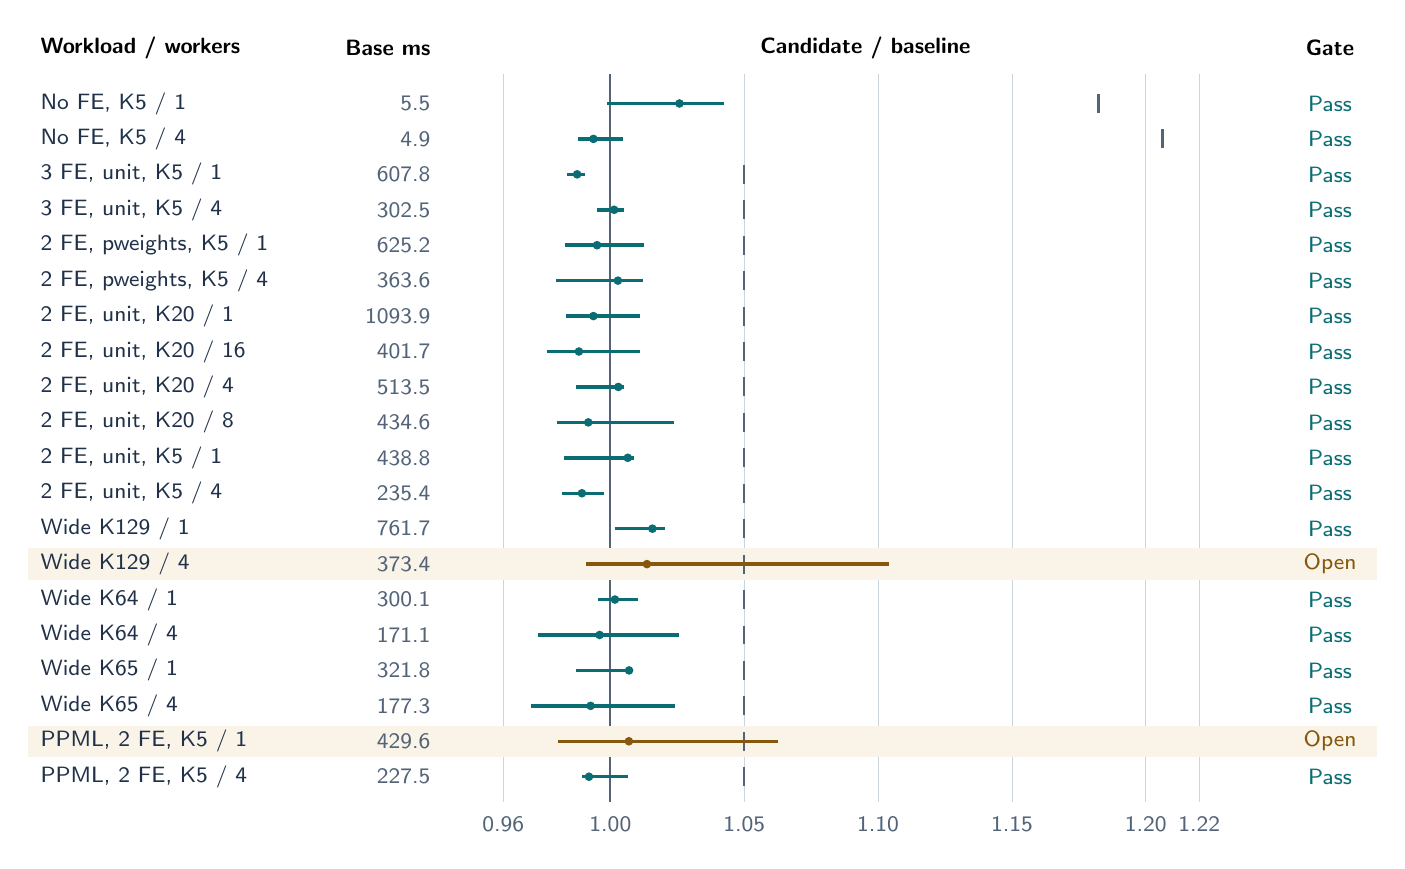
\begin{tikzpicture}[x=1cm,y=1cm,font=\sffamily\fontsize{8.4}{10}\selectfont]
\node[anchor=west,font=\sffamily\bfseries\fontsize{8.3}{10}\selectfont] at (0,0.48) {Workload / workers};
\node[anchor=east,font=\sffamily\bfseries\fontsize{8.3}{10}\selectfont] at (5.2,0.48) {Base ms};
\node[font=\sffamily\bfseries\fontsize{8.3}{10}\selectfont] at (10.6,0.48) {Candidate / baseline};
\node[font=\sffamily\bfseries\fontsize{8.3}{10}\selectfont] at (16.5,0.48) {Gate};
\draw[Rule,line width=0.30pt] (6.00000,0.15)--(6.00000,-9.1);
\node[text=Muted] at (6.00000,-9.38) {0.96};
\draw[Muted,line width=0.65pt] (7.36000,0.15)--(7.36000,-9.1);
\node[text=Muted] at (7.36000,-9.38) {1.00};
\draw[Rule,line width=0.30pt] (9.06000,0.15)--(9.06000,-9.1);
\node[text=Muted] at (9.06000,-9.38) {1.05};
\draw[Rule,line width=0.30pt] (10.76000,0.15)--(10.76000,-9.1);
\node[text=Muted] at (10.76000,-9.38) {1.10};
\draw[Rule,line width=0.30pt] (12.46000,0.15)--(12.46000,-9.1);
\node[text=Muted] at (12.46000,-9.38) {1.15};
\draw[Rule,line width=0.30pt] (14.16000,0.15)--(14.16000,-9.1);
\node[text=Muted] at (14.16000,-9.38) {1.20};
\draw[Rule,line width=0.30pt] (14.84000,0.15)--(14.84000,-9.1);
\node[text=Muted] at (14.84000,-9.38) {1.22};
\node[anchor=west,text=Ink] at (0,-0.22500) {No FE, K5 / 1};
\node[anchor=east,text=Muted] at (5.2,-0.22500) {5.5};
\draw[Muted,line width=.9pt] (13.56212,-0.34500)--(13.56212,-0.10500);
\draw[Teal,line width=1.25pt] (7.32280,-0.22500)--(8.79999,-0.22500);
\fill[Teal] (8.23746,-0.22500) circle (0.055cm);
\node[text=Teal] at (16.5,-0.22500) {Pass};
\node[anchor=west,text=Ink] at (0,-0.67500) {No FE, K5 / 4};
\node[anchor=east,text=Muted] at (5.2,-0.67500) {4.9};
\draw[Muted,line width=.9pt] (14.37031,-0.79500)--(14.37031,-0.55500);
\draw[Teal,line width=1.25pt] (6.94639,-0.67500)--(7.52271,-0.67500);
\fill[Teal] (7.14516,-0.67500) circle (0.055cm);
\node[text=Teal] at (16.5,-0.67500) {Pass};
\node[anchor=west,text=Ink] at (0,-1.12500) {3 FE, unit, K5 / 1};
\node[anchor=east,text=Muted] at (5.2,-1.12500) {607.8};
\draw[Muted,line width=.9pt] (9.06000,-1.24500)--(9.06000,-1.00500);
\draw[Teal,line width=1.25pt] (6.81166,-1.12500)--(7.03394,-1.12500);
\fill[Teal] (6.93812,-1.12500) circle (0.055cm);
\node[text=Teal] at (16.5,-1.12500) {Pass};
\node[anchor=west,text=Ink] at (0,-1.57500) {3 FE, unit, K5 / 4};
\node[anchor=east,text=Muted] at (5.2,-1.57500) {302.5};
\draw[Muted,line width=.9pt] (9.06000,-1.69500)--(9.06000,-1.45500);
\draw[Teal,line width=1.25pt] (7.19666,-1.57500)--(7.53262,-1.57500);
\fill[Teal] (7.40845,-1.57500) circle (0.055cm);
\node[text=Teal] at (16.5,-1.57500) {Pass};
\node[anchor=west,text=Ink] at (0,-2.02500) {2 FE, pweights, K5 / 1};
\node[anchor=east,text=Muted] at (5.2,-2.02500) {625.2};
\draw[Muted,line width=.9pt] (9.06000,-2.14500)--(9.06000,-1.90500);
\draw[Teal,line width=1.25pt] (6.78970,-2.02500)--(7.79057,-2.02500);
\fill[Teal] (7.19147,-2.02500) circle (0.055cm);
\node[text=Teal] at (16.5,-2.02500) {Pass};
\node[anchor=west,text=Ink] at (0,-2.47500) {2 FE, pweights, K5 / 4};
\node[anchor=east,text=Muted] at (5.2,-2.47500) {363.6};
\draw[Muted,line width=.9pt] (9.06000,-2.59500)--(9.06000,-2.35500);
\draw[Teal,line width=1.25pt] (6.66380,-2.47500)--(7.77304,-2.47500);
\fill[Teal] (7.45580,-2.47500) circle (0.055cm);
\node[text=Teal] at (16.5,-2.47500) {Pass};
\node[anchor=west,text=Ink] at (0,-2.92500) {2 FE, unit, K20 / 1};
\node[anchor=east,text=Muted] at (5.2,-2.92500) {1093.9};
\draw[Muted,line width=.9pt] (9.06000,-3.04500)--(9.06000,-2.80500);
\draw[Teal,line width=1.25pt] (6.79946,-2.92500)--(7.73025,-2.92500);
\fill[Teal] (7.14473,-2.92500) circle (0.055cm);
\node[text=Teal] at (16.5,-2.92500) {Pass};
\node[anchor=west,text=Ink] at (0,-3.37500) {2 FE, unit, K20 / 16};
\node[anchor=east,text=Muted] at (5.2,-3.37500) {401.7};
\draw[Muted,line width=.9pt] (9.06000,-3.49500)--(9.06000,-3.25500);
\draw[Teal,line width=1.25pt] (6.56160,-3.37500)--(7.73820,-3.37500);
\fill[Teal] (6.96069,-3.37500) circle (0.055cm);
\node[text=Teal] at (16.5,-3.37500) {Pass};
\node[anchor=west,text=Ink] at (0,-3.82500) {2 FE, unit, K20 / 4};
\node[anchor=east,text=Muted] at (5.2,-3.82500) {513.5};
\draw[Muted,line width=.9pt] (9.06000,-3.94500)--(9.06000,-3.70500);
\draw[Teal,line width=1.25pt] (6.92380,-3.82500)--(7.52752,-3.82500);
\fill[Teal] (7.46118,-3.82500) circle (0.055cm);
\node[text=Teal] at (16.5,-3.82500) {Pass};
\node[anchor=west,text=Ink] at (0,-4.27500) {2 FE, unit, K20 / 8};
\node[anchor=east,text=Muted] at (5.2,-4.27500) {434.6};
\draw[Muted,line width=.9pt] (9.06000,-4.39500)--(9.06000,-4.15500);
\draw[Teal,line width=1.25pt] (6.67931,-4.27500)--(8.16563,-4.27500);
\fill[Teal] (7.07961,-4.27500) circle (0.055cm);
\node[text=Teal] at (16.5,-4.27500) {Pass};
\node[anchor=west,text=Ink] at (0,-4.72500) {2 FE, unit, K5 / 1};
\node[anchor=east,text=Muted] at (5.2,-4.72500) {438.8};
\draw[Muted,line width=.9pt] (9.06000,-4.84500)--(9.06000,-4.60500);
\draw[Teal,line width=1.25pt] (6.76676,-4.72500)--(7.66656,-4.72500);
\fill[Teal] (7.58130,-4.72500) circle (0.055cm);
\node[text=Teal] at (16.5,-4.72500) {Pass};
\node[anchor=west,text=Ink] at (0,-5.17500) {2 FE, unit, K5 / 4};
\node[anchor=east,text=Muted] at (5.2,-5.17500) {235.4};
\draw[Muted,line width=.9pt] (9.06000,-5.29500)--(9.06000,-5.05500);
\draw[Teal,line width=1.25pt] (6.75128,-5.17500)--(7.28018,-5.17500);
\fill[Teal] (6.99905,-5.17500) circle (0.055cm);
\node[text=Teal] at (16.5,-5.17500) {Pass};
\node[anchor=west,text=Ink] at (0,-5.62500) {Wide K129 / 1};
\node[anchor=east,text=Muted] at (5.2,-5.62500) {761.7};
\draw[Muted,line width=.9pt] (9.06000,-5.74500)--(9.06000,-5.50500);
\draw[Teal,line width=1.25pt] (7.41477,-5.62500)--(8.05362,-5.62500);
\fill[Teal] (7.89389,-5.62500) circle (0.055cm);
\node[text=Teal] at (16.5,-5.62500) {Pass};
\fill[Warm] (-0.04,-6.27500) rectangle (17.1,-5.87500);
\node[anchor=west,text=Ink] at (0,-6.07500) {Wide K129 / 4};
\node[anchor=east,text=Muted] at (5.2,-6.07500) {373.4};
\draw[Muted,line width=.9pt] (9.06000,-6.19500)--(9.06000,-5.95500);
\draw[Amber,line width=1.25pt] (7.05230,-6.07500)--(10.89274,-6.07500);
\fill[Amber] (7.82459,-6.07500) circle (0.055cm);
\node[text=Amber] at (16.5,-6.07500) {Open};
\node[anchor=west,text=Ink] at (0,-6.52500) {Wide K64 / 1};
\node[anchor=east,text=Muted] at (5.2,-6.52500) {300.1};
\draw[Muted,line width=.9pt] (9.06000,-6.64500)--(9.06000,-6.40500);
\draw[Teal,line width=1.25pt] (7.20907,-6.52500)--(7.71707,-6.52500);
\fill[Teal] (7.41814,-6.52500) circle (0.055cm);
\node[text=Teal] at (16.5,-6.52500) {Pass};
\node[anchor=west,text=Ink] at (0,-6.97500) {Wide K64 / 4};
\node[anchor=east,text=Muted] at (5.2,-6.97500) {171.1};
\draw[Muted,line width=.9pt] (9.06000,-7.09500)--(9.06000,-6.85500);
\draw[Teal,line width=1.25pt] (6.43795,-6.97500)--(8.22700,-6.97500);
\fill[Teal] (7.22384,-6.97500) circle (0.055cm);
\node[text=Teal] at (16.5,-6.97500) {Pass};
\node[anchor=west,text=Ink] at (0,-7.42500) {Wide K65 / 1};
\node[anchor=east,text=Muted] at (5.2,-7.42500) {321.8};
\draw[Muted,line width=.9pt] (9.06000,-7.54500)--(9.06000,-7.30500);
\draw[Teal,line width=1.25pt] (6.92381,-7.42500)--(7.64569,-7.42500);
\fill[Teal] (7.59761,-7.42500) circle (0.055cm);
\node[text=Teal] at (16.5,-7.42500) {Pass};
\node[anchor=west,text=Ink] at (0,-7.87500) {Wide K65 / 4};
\node[anchor=east,text=Muted] at (5.2,-7.87500) {177.3};
\draw[Muted,line width=.9pt] (9.06000,-7.99500)--(9.06000,-7.75500);
\draw[Teal,line width=1.25pt] (6.35349,-7.87500)--(8.18544,-7.87500);
\fill[Teal] (7.10922,-7.87500) circle (0.055cm);
\node[text=Teal] at (16.5,-7.87500) {Pass};
\fill[Warm] (-0.04,-8.52500) rectangle (17.1,-8.12500);
\node[anchor=west,text=Ink] at (0,-8.32500) {PPML, 2 FE, K5 / 1};
\node[anchor=east,text=Muted] at (5.2,-8.32500) {429.6};
\draw[Muted,line width=.9pt] (9.06000,-8.44500)--(9.06000,-8.20500);
\draw[Amber,line width=1.25pt] (6.69689,-8.32500)--(9.48696,-8.32500);
\fill[Amber] (7.59555,-8.32500) circle (0.055cm);
\node[text=Amber] at (16.5,-8.32500) {Open};
\node[anchor=west,text=Ink] at (0,-8.77500) {PPML, 2 FE, K5 / 4};
\node[anchor=east,text=Muted] at (5.2,-8.77500) {227.5};
\draw[Muted,line width=.9pt] (9.06000,-8.89500)--(9.06000,-8.65500);
\draw[Teal,line width=1.25pt] (7.00388,-8.77500)--(7.58810,-8.77500);
\fill[Teal] (7.08834,-8.77500) circle (0.055cm);
\node[text=Teal] at (16.5,-8.77500) {Pass};

\end{tikzpicture}
\end{center}
{\smallbody
\begin{tabularx}{\linewidth}{Y P{0.15\linewidth}P{0.28\linewidth}P{0.11\linewidth}}
\toprule
\textbf{Unresolved cell} & \textbf{Median ratio} & \textbf{Nominal 95\% interval} & \textbf{Cap}\\
\midrule
Wide K129 / four workers & 1.013664 & [0.990950, 1.103904] & 1.050\\
PPML / one worker & 1.006928 & [0.980497, 1.062558] & 1.050\\
\bottomrule
\end{tabularx}
The cap is $1+\max(0.05,0.001/\operatorname{median}(t_{\rm baseline}))$. Its one-millisecond term permits 1.182 and 1.206 on the short no-FE cells; all other caps are 1.05. A cell passes only when its interval's upper endpoint meets the cap. Intervals are not simultaneous or universal guarantees.

The quiet observations ran 06:49:36--07:00:30 local time, before the observed storage-process start. Later contamination does not invalidate this earlier run. Its two original nonpasses are preserved; the later pooled decisions are on page 21.
}
\anchor{Retained observations: \code{bench/results/solver-routing-20261014.json}, \code{standard}. Original summary SHA-256 begins \code{3514797d}; full hashes, timings and fingerprints are retained.}

% PAGE 19 ---------------------------------------------------------------------
% Exploratory ablation heatmap; deliberately no selection or significance claims.
\newleaf
\sect{18 / EXPLORATORY ABLATIONS}{Observed ratios across the two-FE frontier}
\tagline{Codex results figure. All 26 cells shown; this is not quiet-host performance qualification.}
\begin{binding}\smallbody
A storage-management process began during this panel. All timings below are \textbf{exploratory}; the evidence cannot identify which cells were affected. Three paired measurements per arm do not authorize a ranking, policy selection or reliable speedup claim.
\end{binding}
{\smallbody Each entry is the recorded median paired ratio to baseline. Colors show log-ratio magnitude, clipped at $\times4$ and $\div4$; they do not encode significance or a passing gate. Baseline medians are in milliseconds.}
\begin{center}
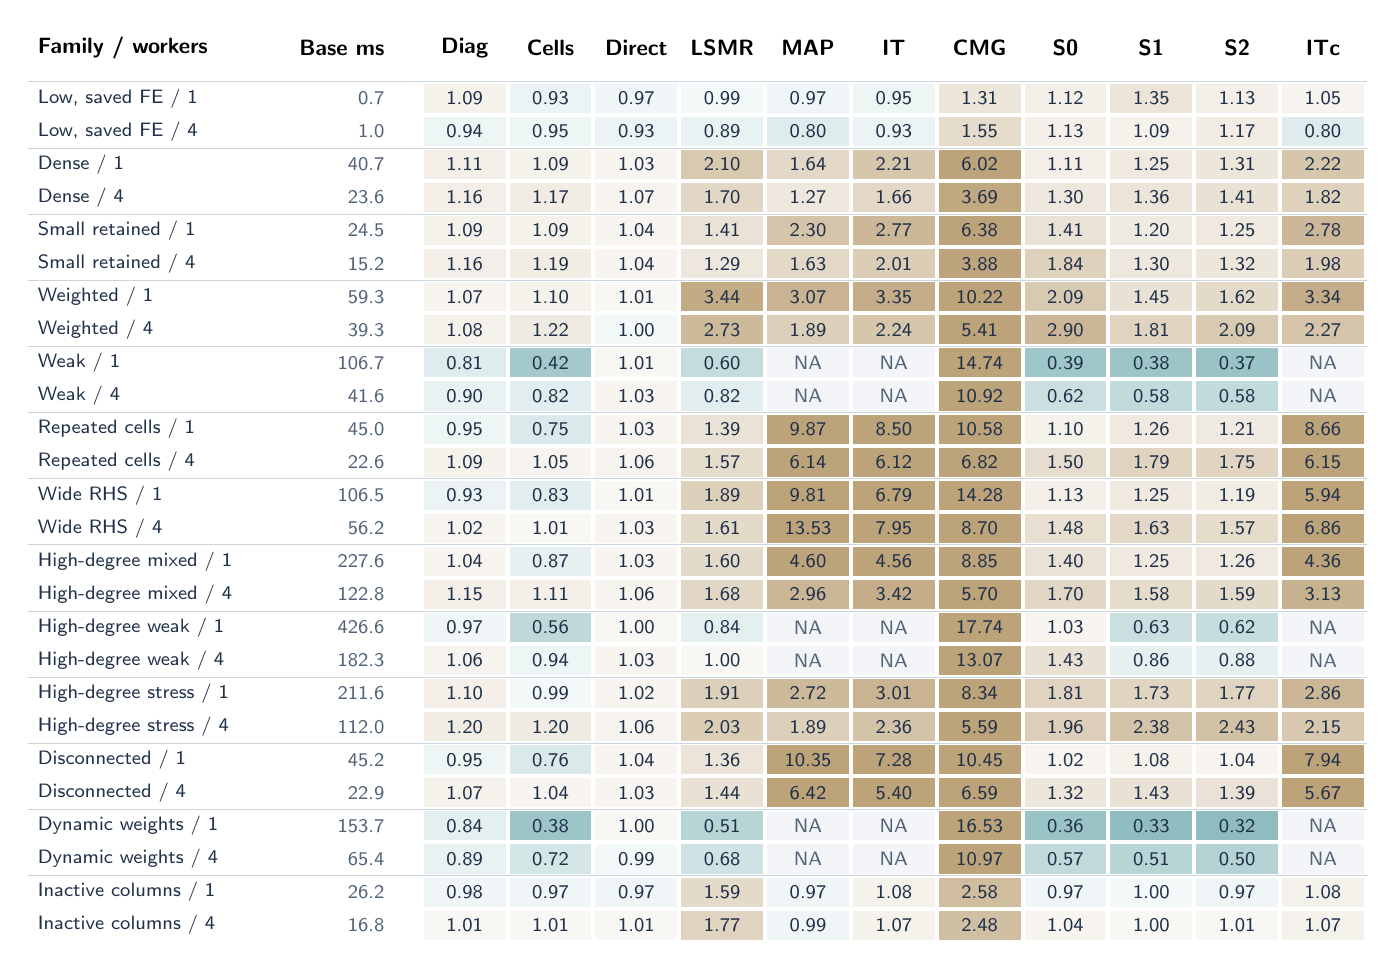
\begin{tikzpicture}[x=1cm,y=1cm,font=\sffamily\fontsize{7.5}{9}\selectfont]
\node[anchor=west,font=\sffamily\bfseries\fontsize{8}{10}\selectfont] at (0,0.43) {Family / workers};
\node[anchor=east,font=\sffamily\bfseries\fontsize{8}{10}\selectfont] at (4.65,0.43) {Base ms};
\node[font=\sffamily\bfseries\fontsize{7.8}{9}\selectfont] at (5.5450,0.43) {Diag};
\node[font=\sffamily\bfseries\fontsize{7.8}{9}\selectfont] at (6.6350,0.43) {Cells};
\node[font=\sffamily\bfseries\fontsize{7.8}{9}\selectfont] at (7.7250,0.43) {Direct};
\node[font=\sffamily\bfseries\fontsize{7.8}{9}\selectfont] at (8.8150,0.43) {LSMR};
\node[font=\sffamily\bfseries\fontsize{7.8}{9}\selectfont] at (9.9050,0.43) {MAP};
\node[font=\sffamily\bfseries\fontsize{7.8}{9}\selectfont] at (10.9950,0.43) {IT};
\node[font=\sffamily\bfseries\fontsize{7.8}{9}\selectfont] at (12.0850,0.43) {CMG};
\node[font=\sffamily\bfseries\fontsize{7.8}{9}\selectfont] at (13.1750,0.43) {S0};
\node[font=\sffamily\bfseries\fontsize{7.8}{9}\selectfont] at (14.2650,0.43) {S1};
\node[font=\sffamily\bfseries\fontsize{7.8}{9}\selectfont] at (15.3550,0.43) {S2};
\node[font=\sffamily\bfseries\fontsize{7.8}{9}\selectfont] at (16.4450,0.43) {ITc};
\draw[Rule,line width=.3pt] (0,0.0000)--(17.0,0.0000);
\node[anchor=west,text=Ink] at (0,-0.2100) {Low, saved FE / 1};
\node[anchor=east,text=Muted] at (4.65,-0.2100) {0.7};
\fill[Amber!8] (5.0250,-0.3950) rectangle (6.0650,-0.0250);
\node[text=Ink] at (5.5450,-0.2100) {1.09};
\fill[Teal!8] (6.1150,-0.3950) rectangle (7.1550,-0.0250);
\node[text=Ink] at (6.6350,-0.2100) {0.93};
\fill[Teal!6] (7.2050,-0.3950) rectangle (8.2450,-0.0250);
\node[text=Ink] at (7.7250,-0.2100) {0.97};
\fill[Teal!5] (8.2950,-0.3950) rectangle (9.3350,-0.0250);
\node[text=Ink] at (8.8150,-0.2100) {0.99};
\fill[Teal!6] (9.3850,-0.3950) rectangle (10.4250,-0.0250);
\node[text=Ink] at (9.9050,-0.2100) {0.97};
\fill[Teal!7] (10.4750,-0.3950) rectangle (11.5150,-0.0250);
\node[text=Ink] at (10.9950,-0.2100) {0.95};
\fill[Amber!15] (11.5650,-0.3950) rectangle (12.6050,-0.0250);
\node[text=Ink] at (12.0850,-0.2100) {1.31};
\fill[Amber!9] (12.6550,-0.3950) rectangle (13.6950,-0.0250);
\node[text=Ink] at (13.1750,-0.2100) {1.12};
\fill[Amber!16] (13.7450,-0.3950) rectangle (14.7850,-0.0250);
\node[text=Ink] at (14.2650,-0.2100) {1.35};
\fill[Amber!10] (14.8350,-0.3950) rectangle (15.8750,-0.0250);
\node[text=Ink] at (15.3550,-0.2100) {1.13};
\fill[Amber!7] (15.9250,-0.3950) rectangle (16.9650,-0.0250);
\node[text=Ink] at (16.4450,-0.2100) {1.05};
\node[anchor=west,text=Ink] at (0,-0.6300) {Low, saved FE / 4};
\node[anchor=east,text=Muted] at (4.65,-0.6300) {1.0};
\fill[Teal!7] (5.0250,-0.8150) rectangle (6.0650,-0.4450);
\node[text=Ink] at (5.5450,-0.6300) {0.94};
\fill[Teal!7] (6.1150,-0.8150) rectangle (7.1550,-0.4450);
\node[text=Ink] at (6.6350,-0.6300) {0.95};
\fill[Teal!8] (7.2050,-0.8150) rectangle (8.2450,-0.4450);
\node[text=Ink] at (7.7250,-0.6300) {0.93};
\fill[Teal!9] (8.2950,-0.8150) rectangle (9.3350,-0.4450);
\node[text=Ink] at (8.8150,-0.6300) {0.89};
\fill[Teal!13] (9.3850,-0.8150) rectangle (10.4250,-0.4450);
\node[text=Ink] at (9.9050,-0.6300) {0.80};
\fill[Teal!8] (10.4750,-0.8150) rectangle (11.5150,-0.4450);
\node[text=Ink] at (10.9950,-0.6300) {0.93};
\fill[Amber!21] (11.5650,-0.8150) rectangle (12.6050,-0.4450);
\node[text=Ink] at (12.0850,-0.6300) {1.55};
\fill[Amber!9] (12.6550,-0.8150) rectangle (13.6950,-0.4450);
\node[text=Ink] at (13.1750,-0.6300) {1.13};
\fill[Amber!8] (13.7450,-0.8150) rectangle (14.7850,-0.4450);
\node[text=Ink] at (14.2650,-0.6300) {1.09};
\fill[Amber!11] (14.8350,-0.8150) rectangle (15.8750,-0.4450);
\node[text=Ink] at (15.3550,-0.6300) {1.17};
\fill[Teal!13] (15.9250,-0.8150) rectangle (16.9650,-0.4450);
\node[text=Ink] at (16.4450,-0.6300) {0.80};
\draw[Rule,line width=.3pt] (0,-0.8400)--(17.0,-0.8400);
\node[anchor=west,text=Ink] at (0,-1.0500) {Dense / 1};
\node[anchor=east,text=Muted] at (4.65,-1.0500) {40.7};
\fill[Amber!9] (5.0250,-1.2350) rectangle (6.0650,-0.8650);
\node[text=Ink] at (5.5450,-1.0500) {1.11};
\fill[Amber!8] (6.1150,-1.2350) rectangle (7.1550,-0.8650);
\node[text=Ink] at (6.6350,-1.0500) {1.09};
\fill[Amber!6] (7.2050,-1.2350) rectangle (8.2450,-0.8650);
\node[text=Ink] at (7.7250,-1.0500) {1.03};
\fill[Amber!32] (8.2950,-1.2350) rectangle (9.3350,-0.8650);
\node[text=Ink] at (8.8150,-1.0500) {2.10};
\fill[Amber!23] (9.3850,-1.2350) rectangle (10.4250,-0.8650);
\node[text=Ink] at (9.9050,-1.0500) {1.64};
\fill[Amber!34] (10.4750,-1.2350) rectangle (11.5150,-0.8650);
\node[text=Ink] at (10.9950,-1.0500) {2.21};
\fill[Amber!55] (11.5650,-1.2350) rectangle (12.6050,-0.8650);
\node[text=Ink] at (12.0850,-1.0500) {6.02};
\fill[Amber!9] (12.6550,-1.2350) rectangle (13.6950,-0.8650);
\node[text=Ink] at (13.1750,-1.0500) {1.11};
\fill[Amber!13] (13.7450,-1.2350) rectangle (14.7850,-0.8650);
\node[text=Ink] at (14.2650,-1.0500) {1.25};
\fill[Amber!15] (14.8350,-1.2350) rectangle (15.8750,-0.8650);
\node[text=Ink] at (15.3550,-1.0500) {1.31};
\fill[Amber!34] (15.9250,-1.2350) rectangle (16.9650,-0.8650);
\node[text=Ink] at (16.4450,-1.0500) {2.22};
\node[anchor=west,text=Ink] at (0,-1.4700) {Dense / 4};
\node[anchor=east,text=Muted] at (4.65,-1.4700) {23.6};
\fill[Amber!10] (5.0250,-1.6550) rectangle (6.0650,-1.2850);
\node[text=Ink] at (5.5450,-1.4700) {1.16};
\fill[Amber!11] (6.1150,-1.6550) rectangle (7.1550,-1.2850);
\node[text=Ink] at (6.6350,-1.4700) {1.17};
\fill[Amber!7] (7.2050,-1.6550) rectangle (8.2450,-1.2850);
\node[text=Ink] at (7.7250,-1.4700) {1.07};
\fill[Amber!24] (8.2950,-1.6550) rectangle (9.3350,-1.2850);
\node[text=Ink] at (8.8150,-1.4700) {1.70};
\fill[Amber!14] (9.3850,-1.6550) rectangle (10.4250,-1.2850);
\node[text=Ink] at (9.9050,-1.4700) {1.27};
\fill[Amber!23] (10.4750,-1.6550) rectangle (11.5150,-1.2850);
\node[text=Ink] at (10.9950,-1.4700) {1.66};
\fill[Amber!52] (11.5650,-1.6550) rectangle (12.6050,-1.2850);
\node[text=Ink] at (12.0850,-1.4700) {3.69};
\fill[Amber!14] (12.6550,-1.6550) rectangle (13.6950,-1.2850);
\node[text=Ink] at (13.1750,-1.4700) {1.30};
\fill[Amber!16] (13.7450,-1.6550) rectangle (14.7850,-1.2850);
\node[text=Ink] at (14.2650,-1.4700) {1.36};
\fill[Amber!18] (14.8350,-1.6550) rectangle (15.8750,-1.2850);
\node[text=Ink] at (15.3550,-1.4700) {1.41};
\fill[Amber!27] (15.9250,-1.6550) rectangle (16.9650,-1.2850);
\node[text=Ink] at (16.4450,-1.4700) {1.82};
\draw[Rule,line width=.3pt] (0,-1.6800)--(17.0,-1.6800);
\node[anchor=west,text=Ink] at (0,-1.8900) {Small retained / 1};
\node[anchor=east,text=Muted] at (4.65,-1.8900) {24.5};
\fill[Amber!8] (5.0250,-2.0750) rectangle (6.0650,-1.7050);
\node[text=Ink] at (5.5450,-1.8900) {1.09};
\fill[Amber!8] (6.1150,-2.0750) rectangle (7.1550,-1.7050);
\node[text=Ink] at (6.6350,-1.8900) {1.09};
\fill[Amber!6] (7.2050,-2.0750) rectangle (8.2450,-1.7050);
\node[text=Ink] at (7.7250,-1.8900) {1.04};
\fill[Amber!17] (8.2950,-2.0750) rectangle (9.3350,-1.7050);
\node[text=Ink] at (8.8150,-1.8900) {1.41};
\fill[Amber!35] (9.3850,-2.0750) rectangle (10.4250,-1.7050);
\node[text=Ink] at (9.9050,-1.8900) {2.30};
\fill[Amber!42] (10.4750,-2.0750) rectangle (11.5150,-1.7050);
\node[text=Ink] at (10.9950,-1.8900) {2.77};
\fill[Amber!55] (11.5650,-2.0750) rectangle (12.6050,-1.7050);
\node[text=Ink] at (12.0850,-1.8900) {6.38};
\fill[Amber!17] (12.6550,-2.0750) rectangle (13.6950,-1.7050);
\node[text=Ink] at (13.1750,-1.8900) {1.41};
\fill[Amber!12] (13.7450,-2.0750) rectangle (14.7850,-1.7050);
\node[text=Ink] at (14.2650,-1.8900) {1.20};
\fill[Amber!13] (14.8350,-2.0750) rectangle (15.8750,-1.7050);
\node[text=Ink] at (15.3550,-1.8900) {1.25};
\fill[Amber!42] (15.9250,-2.0750) rectangle (16.9650,-1.7050);
\node[text=Ink] at (16.4450,-1.8900) {2.78};
\node[anchor=west,text=Ink] at (0,-2.3100) {Small retained / 4};
\node[anchor=east,text=Muted] at (4.65,-2.3100) {15.2};
\fill[Amber!10] (5.0250,-2.4950) rectangle (6.0650,-2.1250);
\node[text=Ink] at (5.5450,-2.3100) {1.16};
\fill[Amber!11] (6.1150,-2.4950) rectangle (7.1550,-2.1250);
\node[text=Ink] at (6.6350,-2.3100) {1.19};
\fill[Amber!6] (7.2050,-2.4950) rectangle (8.2450,-2.1250);
\node[text=Ink] at (7.7250,-2.3100) {1.04};
\fill[Amber!14] (8.2950,-2.4950) rectangle (9.3350,-2.1250);
\node[text=Ink] at (8.8150,-2.3100) {1.29};
\fill[Amber!23] (9.3850,-2.4950) rectangle (10.4250,-2.1250);
\node[text=Ink] at (9.9050,-2.3100) {1.63};
\fill[Amber!30] (10.4750,-2.4950) rectangle (11.5150,-2.1250);
\node[text=Ink] at (10.9950,-2.3100) {2.01};
\fill[Amber!54] (11.5650,-2.4950) rectangle (12.6050,-2.1250);
\node[text=Ink] at (12.0850,-2.3100) {3.88};
\fill[Amber!27] (12.6550,-2.4950) rectangle (13.6950,-2.1250);
\node[text=Ink] at (13.1750,-2.3100) {1.84};
\fill[Amber!14] (13.7450,-2.4950) rectangle (14.7850,-2.1250);
\node[text=Ink] at (14.2650,-2.3100) {1.30};
\fill[Amber!15] (14.8350,-2.4950) rectangle (15.8750,-2.1250);
\node[text=Ink] at (15.3550,-2.3100) {1.32};
\fill[Amber!30] (15.9250,-2.4950) rectangle (16.9650,-2.1250);
\node[text=Ink] at (16.4450,-2.3100) {1.98};
\draw[Rule,line width=.3pt] (0,-2.5200)--(17.0,-2.5200);
\node[anchor=west,text=Ink] at (0,-2.7300) {Weighted / 1};
\node[anchor=east,text=Muted] at (4.65,-2.7300) {59.3};
\fill[Amber!7] (5.0250,-2.9150) rectangle (6.0650,-2.5450);
\node[text=Ink] at (5.5450,-2.7300) {1.07};
\fill[Amber!8] (6.1150,-2.9150) rectangle (7.1550,-2.5450);
\node[text=Ink] at (6.6350,-2.7300) {1.10};
\fill[Amber!5] (7.2050,-2.9150) rectangle (8.2450,-2.5450);
\node[text=Ink] at (7.7250,-2.7300) {1.01};
\fill[Amber!50] (8.2950,-2.9150) rectangle (9.3350,-2.5450);
\node[text=Ink] at (8.8150,-2.7300) {3.44};
\fill[Amber!45] (9.3850,-2.9150) rectangle (10.4250,-2.5450);
\node[text=Ink] at (9.9050,-2.7300) {3.07};
\fill[Amber!49] (10.4750,-2.9150) rectangle (11.5150,-2.5450);
\node[text=Ink] at (10.9950,-2.7300) {3.35};
\fill[Amber!55] (11.5650,-2.9150) rectangle (12.6050,-2.5450);
\node[text=Ink] at (12.0850,-2.7300) {10.22};
\fill[Amber!32] (12.6550,-2.9150) rectangle (13.6950,-2.5450);
\node[text=Ink] at (13.1750,-2.7300) {2.09};
\fill[Amber!18] (13.7450,-2.9150) rectangle (14.7850,-2.5450);
\node[text=Ink] at (14.2650,-2.7300) {1.45};
\fill[Amber!22] (14.8350,-2.9150) rectangle (15.8750,-2.5450);
\node[text=Ink] at (15.3550,-2.7300) {1.62};
\fill[Amber!49] (15.9250,-2.9150) rectangle (16.9650,-2.5450);
\node[text=Ink] at (16.4450,-2.7300) {3.34};
\node[anchor=west,text=Ink] at (0,-3.1500) {Weighted / 4};
\node[anchor=east,text=Muted] at (4.65,-3.1500) {39.3};
\fill[Amber!8] (5.0250,-3.3350) rectangle (6.0650,-2.9650);
\node[text=Ink] at (5.5450,-3.1500) {1.08};
\fill[Amber!12] (6.1150,-3.3350) rectangle (7.1550,-2.9650);
\node[text=Ink] at (6.6350,-3.1500) {1.22};
\fill[Teal!5] (7.2050,-3.3350) rectangle (8.2450,-2.9650);
\node[text=Ink] at (7.7250,-3.1500) {1.00};
\fill[Amber!41] (8.2950,-3.3350) rectangle (9.3350,-2.9650);
\node[text=Ink] at (8.8150,-3.1500) {2.73};
\fill[Amber!28] (9.3850,-3.3350) rectangle (10.4250,-2.9650);
\node[text=Ink] at (9.9050,-3.1500) {1.89};
\fill[Amber!34] (10.4750,-3.3350) rectangle (11.5150,-2.9650);
\node[text=Ink] at (10.9950,-3.1500) {2.24};
\fill[Amber!55] (11.5650,-3.3350) rectangle (12.6050,-2.9650);
\node[text=Ink] at (12.0850,-3.1500) {5.41};
\fill[Amber!43] (12.6550,-3.3350) rectangle (13.6950,-2.9650);
\node[text=Ink] at (13.1750,-3.1500) {2.90};
\fill[Amber!26] (13.7450,-3.3350) rectangle (14.7850,-2.9650);
\node[text=Ink] at (14.2650,-3.1500) {1.81};
\fill[Amber!32] (14.8350,-3.3350) rectangle (15.8750,-2.9650);
\node[text=Ink] at (15.3550,-3.1500) {2.09};
\fill[Amber!35] (15.9250,-3.3350) rectangle (16.9650,-2.9650);
\node[text=Ink] at (16.4450,-3.1500) {2.27};
\draw[Rule,line width=.3pt] (0,-3.3600)--(17.0,-3.3600);
\node[anchor=west,text=Ink] at (0,-3.5700) {Weak / 1};
\node[anchor=east,text=Muted] at (4.65,-3.5700) {106.7};
\fill[Teal!13] (5.0250,-3.7550) rectangle (6.0650,-3.3850);
\node[text=Ink] at (5.5450,-3.5700) {0.81};
\fill[Teal!37] (6.1150,-3.7550) rectangle (7.1550,-3.3850);
\node[text=Ink] at (6.6350,-3.5700) {0.42};
\fill[Amber!5] (7.2050,-3.7550) rectangle (8.2450,-3.3850);
\node[text=Ink] at (7.7250,-3.5700) {1.01};
\fill[Teal!24] (8.2950,-3.7550) rectangle (9.3350,-3.3850);
\node[text=Ink] at (8.8150,-3.5700) {0.60};
\fill[Light] (9.3850,-3.7550) rectangle (10.4250,-3.3850);
\node[text=Muted] at (9.9050,-3.5700) {NA};
\fill[Light] (10.4750,-3.7550) rectangle (11.5150,-3.3850);
\node[text=Muted] at (10.9950,-3.5700) {NA};
\fill[Amber!55] (11.5650,-3.7550) rectangle (12.6050,-3.3850);
\node[text=Ink] at (12.0850,-3.5700) {14.74};
\fill[Teal!39] (12.6550,-3.7550) rectangle (13.6950,-3.3850);
\node[text=Ink] at (13.1750,-3.5700) {0.39};
\fill[Teal!40] (13.7450,-3.7550) rectangle (14.7850,-3.3850);
\node[text=Ink] at (14.2650,-3.5700) {0.38};
\fill[Teal!41] (14.8350,-3.7550) rectangle (15.8750,-3.3850);
\node[text=Ink] at (15.3550,-3.5700) {0.37};
\fill[Light] (15.9250,-3.7550) rectangle (16.9650,-3.3850);
\node[text=Muted] at (16.4450,-3.5700) {NA};
\node[anchor=west,text=Ink] at (0,-3.9900) {Weak / 4};
\node[anchor=east,text=Muted] at (4.65,-3.9900) {41.6};
\fill[Teal!9] (5.0250,-4.1750) rectangle (6.0650,-3.8050);
\node[text=Ink] at (5.5450,-3.9900) {0.90};
\fill[Teal!12] (6.1150,-4.1750) rectangle (7.1550,-3.8050);
\node[text=Ink] at (6.6350,-3.9900) {0.82};
\fill[Amber!6] (7.2050,-4.1750) rectangle (8.2450,-3.8050);
\node[text=Ink] at (7.7250,-3.9900) {1.03};
\fill[Teal!12] (8.2950,-4.1750) rectangle (9.3350,-3.8050);
\node[text=Ink] at (8.8150,-3.9900) {0.82};
\fill[Light] (9.3850,-4.1750) rectangle (10.4250,-3.8050);
\node[text=Muted] at (9.9050,-3.9900) {NA};
\fill[Light] (10.4750,-4.1750) rectangle (11.5150,-3.8050);
\node[text=Muted] at (10.9950,-3.9900) {NA};
\fill[Amber!55] (11.5650,-4.1750) rectangle (12.6050,-3.8050);
\node[text=Ink] at (12.0850,-3.9900) {10.92};
\fill[Teal!22] (12.6550,-4.1750) rectangle (13.6950,-3.8050);
\node[text=Ink] at (13.1750,-3.9900) {0.62};
\fill[Teal!25] (13.7450,-4.1750) rectangle (14.7850,-3.8050);
\node[text=Ink] at (14.2650,-3.9900) {0.58};
\fill[Teal!25] (14.8350,-4.1750) rectangle (15.8750,-3.8050);
\node[text=Ink] at (15.3550,-3.9900) {0.58};
\fill[Light] (15.9250,-4.1750) rectangle (16.9650,-3.8050);
\node[text=Muted] at (16.4450,-3.9900) {NA};
\draw[Rule,line width=.3pt] (0,-4.2000)--(17.0,-4.2000);
\node[anchor=west,text=Ink] at (0,-4.4100) {Repeated cells / 1};
\node[anchor=east,text=Muted] at (4.65,-4.4100) {45.0};
\fill[Teal!7] (5.0250,-4.5950) rectangle (6.0650,-4.2250);
\node[text=Ink] at (5.5450,-4.4100) {0.95};
\fill[Teal!15] (6.1150,-4.5950) rectangle (7.1550,-4.2250);
\node[text=Ink] at (6.6350,-4.4100) {0.75};
\fill[Amber!6] (7.2050,-4.5950) rectangle (8.2450,-4.2250);
\node[text=Ink] at (7.7250,-4.4100) {1.03};
\fill[Amber!17] (8.2950,-4.5950) rectangle (9.3350,-4.2250);
\node[text=Ink] at (8.8150,-4.4100) {1.39};
\fill[Amber!55] (9.3850,-4.5950) rectangle (10.4250,-4.2250);
\node[text=Ink] at (9.9050,-4.4100) {9.87};
\fill[Amber!55] (10.4750,-4.5950) rectangle (11.5150,-4.2250);
\node[text=Ink] at (10.9950,-4.4100) {8.50};
\fill[Amber!55] (11.5650,-4.5950) rectangle (12.6050,-4.2250);
\node[text=Ink] at (12.0850,-4.4100) {10.58};
\fill[Amber!8] (12.6550,-4.5950) rectangle (13.6950,-4.2250);
\node[text=Ink] at (13.1750,-4.4100) {1.10};
\fill[Amber!13] (13.7450,-4.5950) rectangle (14.7850,-4.2250);
\node[text=Ink] at (14.2650,-4.4100) {1.26};
\fill[Amber!12] (14.8350,-4.5950) rectangle (15.8750,-4.2250);
\node[text=Ink] at (15.3550,-4.4100) {1.21};
\fill[Amber!55] (15.9250,-4.5950) rectangle (16.9650,-4.2250);
\node[text=Ink] at (16.4450,-4.4100) {8.66};
\node[anchor=west,text=Ink] at (0,-4.8300) {Repeated cells / 4};
\node[anchor=east,text=Muted] at (4.65,-4.8300) {22.6};
\fill[Amber!8] (5.0250,-5.0150) rectangle (6.0650,-4.6450);
\node[text=Ink] at (5.5450,-4.8300) {1.09};
\fill[Amber!7] (6.1150,-5.0150) rectangle (7.1550,-4.6450);
\node[text=Ink] at (6.6350,-4.8300) {1.05};
\fill[Amber!7] (7.2050,-5.0150) rectangle (8.2450,-4.6450);
\node[text=Ink] at (7.7250,-4.8300) {1.06};
\fill[Amber!21] (8.2950,-5.0150) rectangle (9.3350,-4.6450);
\node[text=Ink] at (8.8150,-4.8300) {1.57};
\fill[Amber!55] (9.3850,-5.0150) rectangle (10.4250,-4.6450);
\node[text=Ink] at (9.9050,-4.8300) {6.14};
\fill[Amber!55] (10.4750,-5.0150) rectangle (11.5150,-4.6450);
\node[text=Ink] at (10.9950,-4.8300) {6.12};
\fill[Amber!55] (11.5650,-5.0150) rectangle (12.6050,-4.6450);
\node[text=Ink] at (12.0850,-4.8300) {6.82};
\fill[Amber!20] (12.6550,-5.0150) rectangle (13.6950,-4.6450);
\node[text=Ink] at (13.1750,-4.8300) {1.50};
\fill[Amber!26] (13.7450,-5.0150) rectangle (14.7850,-4.6450);
\node[text=Ink] at (14.2650,-4.8300) {1.79};
\fill[Amber!25] (14.8350,-5.0150) rectangle (15.8750,-4.6450);
\node[text=Ink] at (15.3550,-4.8300) {1.75};
\fill[Amber!55] (15.9250,-5.0150) rectangle (16.9650,-4.6450);
\node[text=Ink] at (16.4450,-4.8300) {6.15};
\draw[Rule,line width=.3pt] (0,-5.0400)--(17.0,-5.0400);
\node[anchor=west,text=Ink] at (0,-5.2500) {Wide RHS / 1};
\node[anchor=east,text=Muted] at (4.65,-5.2500) {106.5};
\fill[Teal!8] (5.0250,-5.4350) rectangle (6.0650,-5.0650);
\node[text=Ink] at (5.5450,-5.2500) {0.93};
\fill[Teal!12] (6.1150,-5.4350) rectangle (7.1550,-5.0650);
\node[text=Ink] at (6.6350,-5.2500) {0.83};
\fill[Amber!5] (7.2050,-5.4350) rectangle (8.2450,-5.0650);
\node[text=Ink] at (7.7250,-5.2500) {1.01};
\fill[Amber!28] (8.2950,-5.4350) rectangle (9.3350,-5.0650);
\node[text=Ink] at (8.8150,-5.2500) {1.89};
\fill[Amber!55] (9.3850,-5.4350) rectangle (10.4250,-5.0650);
\node[text=Ink] at (9.9050,-5.2500) {9.81};
\fill[Amber!55] (10.4750,-5.4350) rectangle (11.5150,-5.0650);
\node[text=Ink] at (10.9950,-5.2500) {6.79};
\fill[Amber!55] (11.5650,-5.4350) rectangle (12.6050,-5.0650);
\node[text=Ink] at (12.0850,-5.2500) {14.28};
\fill[Amber!9] (12.6550,-5.4350) rectangle (13.6950,-5.0650);
\node[text=Ink] at (13.1750,-5.2500) {1.13};
\fill[Amber!13] (13.7450,-5.4350) rectangle (14.7850,-5.0650);
\node[text=Ink] at (14.2650,-5.2500) {1.25};
\fill[Amber!11] (14.8350,-5.4350) rectangle (15.8750,-5.0650);
\node[text=Ink] at (15.3550,-5.2500) {1.19};
\fill[Amber!55] (15.9250,-5.4350) rectangle (16.9650,-5.0650);
\node[text=Ink] at (16.4450,-5.2500) {5.94};
\node[anchor=west,text=Ink] at (0,-5.6700) {Wide RHS / 4};
\node[anchor=east,text=Muted] at (4.65,-5.6700) {56.2};
\fill[Amber!6] (5.0250,-5.8550) rectangle (6.0650,-5.4850);
\node[text=Ink] at (5.5450,-5.6700) {1.02};
\fill[Amber!5] (6.1150,-5.8550) rectangle (7.1550,-5.4850);
\node[text=Ink] at (6.6350,-5.6700) {1.01};
\fill[Amber!6] (7.2050,-5.8550) rectangle (8.2450,-5.4850);
\node[text=Ink] at (7.7250,-5.6700) {1.03};
\fill[Amber!22] (8.2950,-5.8550) rectangle (9.3350,-5.4850);
\node[text=Ink] at (8.8150,-5.6700) {1.61};
\fill[Amber!55] (9.3850,-5.8550) rectangle (10.4250,-5.4850);
\node[text=Ink] at (9.9050,-5.6700) {13.53};
\fill[Amber!55] (10.4750,-5.8550) rectangle (11.5150,-5.4850);
\node[text=Ink] at (10.9950,-5.6700) {7.95};
\fill[Amber!55] (11.5650,-5.8550) rectangle (12.6050,-5.4850);
\node[text=Ink] at (12.0850,-5.6700) {8.70};
\fill[Amber!19] (12.6550,-5.8550) rectangle (13.6950,-5.4850);
\node[text=Ink] at (13.1750,-5.6700) {1.48};
\fill[Amber!23] (13.7450,-5.8550) rectangle (14.7850,-5.4850);
\node[text=Ink] at (14.2650,-5.6700) {1.63};
\fill[Amber!21] (14.8350,-5.8550) rectangle (15.8750,-5.4850);
\node[text=Ink] at (15.3550,-5.6700) {1.57};
\fill[Amber!55] (15.9250,-5.8550) rectangle (16.9650,-5.4850);
\node[text=Ink] at (16.4450,-5.6700) {6.86};
\draw[Rule,line width=.3pt] (0,-5.8800)--(17.0,-5.8800);
\node[anchor=west,text=Ink] at (0,-6.0900) {High-degree mixed / 1};
\node[anchor=east,text=Muted] at (4.65,-6.0900) {227.6};
\fill[Amber!6] (5.0250,-6.2750) rectangle (6.0650,-5.9050);
\node[text=Ink] at (5.5450,-6.0900) {1.04};
\fill[Teal!10] (6.1150,-6.2750) rectangle (7.1550,-5.9050);
\node[text=Ink] at (6.6350,-6.0900) {0.87};
\fill[Amber!6] (7.2050,-6.2750) rectangle (8.2450,-5.9050);
\node[text=Ink] at (7.7250,-6.0900) {1.03};
\fill[Amber!22] (8.2950,-6.2750) rectangle (9.3350,-5.9050);
\node[text=Ink] at (8.8150,-6.0900) {1.60};
\fill[Amber!55] (9.3850,-6.2750) rectangle (10.4250,-5.9050);
\node[text=Ink] at (9.9050,-6.0900) {4.60};
\fill[Amber!55] (10.4750,-6.2750) rectangle (11.5150,-5.9050);
\node[text=Ink] at (10.9950,-6.0900) {4.56};
\fill[Amber!55] (11.5650,-6.2750) rectangle (12.6050,-5.9050);
\node[text=Ink] at (12.0850,-6.0900) {8.85};
\fill[Amber!17] (12.6550,-6.2750) rectangle (13.6950,-5.9050);
\node[text=Ink] at (13.1750,-6.0900) {1.40};
\fill[Amber!13] (13.7450,-6.2750) rectangle (14.7850,-5.9050);
\node[text=Ink] at (14.2650,-6.0900) {1.25};
\fill[Amber!13] (14.8350,-6.2750) rectangle (15.8750,-5.9050);
\node[text=Ink] at (15.3550,-6.0900) {1.26};
\fill[Amber!55] (15.9250,-6.2750) rectangle (16.9650,-5.9050);
\node[text=Ink] at (16.4450,-6.0900) {4.36};
\node[anchor=west,text=Ink] at (0,-6.5100) {High-degree mixed / 4};
\node[anchor=east,text=Muted] at (4.65,-6.5100) {122.8};
\fill[Amber!10] (5.0250,-6.6950) rectangle (6.0650,-6.3250);
\node[text=Ink] at (5.5450,-6.5100) {1.15};
\fill[Amber!9] (6.1150,-6.6950) rectangle (7.1550,-6.3250);
\node[text=Ink] at (6.6350,-6.5100) {1.11};
\fill[Amber!7] (7.2050,-6.6950) rectangle (8.2450,-6.3250);
\node[text=Ink] at (7.7250,-6.5100) {1.06};
\fill[Amber!24] (8.2950,-6.6950) rectangle (9.3350,-6.3250);
\node[text=Ink] at (8.8150,-6.5100) {1.68};
\fill[Amber!44] (9.3850,-6.6950) rectangle (10.4250,-6.3250);
\node[text=Ink] at (9.9050,-6.5100) {2.96};
\fill[Amber!49] (10.4750,-6.6950) rectangle (11.5150,-6.3250);
\node[text=Ink] at (10.9950,-6.5100) {3.42};
\fill[Amber!55] (11.5650,-6.6950) rectangle (12.6050,-6.3250);
\node[text=Ink] at (12.0850,-6.5100) {5.70};
\fill[Amber!24] (12.6550,-6.6950) rectangle (13.6950,-6.3250);
\node[text=Ink] at (13.1750,-6.5100) {1.70};
\fill[Amber!21] (13.7450,-6.6950) rectangle (14.7850,-6.3250);
\node[text=Ink] at (14.2650,-6.5100) {1.58};
\fill[Amber!22] (14.8350,-6.6950) rectangle (15.8750,-6.3250);
\node[text=Ink] at (15.3550,-6.5100) {1.59};
\fill[Amber!46] (15.9250,-6.6950) rectangle (16.9650,-6.3250);
\node[text=Ink] at (16.4450,-6.5100) {3.13};
\draw[Rule,line width=.3pt] (0,-6.7200)--(17.0,-6.7200);
\node[anchor=west,text=Ink] at (0,-6.9300) {High-degree weak / 1};
\node[anchor=east,text=Muted] at (4.65,-6.9300) {426.6};
\fill[Teal!6] (5.0250,-7.1150) rectangle (6.0650,-6.7450);
\node[text=Ink] at (5.5450,-6.9300) {0.97};
\fill[Teal!26] (6.1150,-7.1150) rectangle (7.1550,-6.7450);
\node[text=Ink] at (6.6350,-6.9300) {0.56};
\fill[Amber!5] (7.2050,-7.1150) rectangle (8.2450,-6.7450);
\node[text=Ink] at (7.7250,-6.9300) {1.00};
\fill[Teal!11] (8.2950,-7.1150) rectangle (9.3350,-6.7450);
\node[text=Ink] at (8.8150,-6.9300) {0.84};
\fill[Light] (9.3850,-7.1150) rectangle (10.4250,-6.7450);
\node[text=Muted] at (9.9050,-6.9300) {NA};
\fill[Light] (10.4750,-7.1150) rectangle (11.5150,-6.7450);
\node[text=Muted] at (10.9950,-6.9300) {NA};
\fill[Amber!55] (11.5650,-7.1150) rectangle (12.6050,-6.7450);
\node[text=Ink] at (12.0850,-6.9300) {17.74};
\fill[Amber!6] (12.6550,-7.1150) rectangle (13.6950,-6.7450);
\node[text=Ink] at (13.1750,-6.9300) {1.03};
\fill[Teal!22] (13.7450,-7.1150) rectangle (14.7850,-6.7450);
\node[text=Ink] at (14.2650,-6.9300) {0.63};
\fill[Teal!23] (14.8350,-7.1150) rectangle (15.8750,-6.7450);
\node[text=Ink] at (15.3550,-6.9300) {0.62};
\fill[Light] (15.9250,-7.1150) rectangle (16.9650,-6.7450);
\node[text=Muted] at (16.4450,-6.9300) {NA};
\node[anchor=west,text=Ink] at (0,-7.3500) {High-degree weak / 4};
\node[anchor=east,text=Muted] at (4.65,-7.3500) {182.3};
\fill[Amber!7] (5.0250,-7.5350) rectangle (6.0650,-7.1650);
\node[text=Ink] at (5.5450,-7.3500) {1.06};
\fill[Teal!7] (6.1150,-7.5350) rectangle (7.1550,-7.1650);
\node[text=Ink] at (6.6350,-7.3500) {0.94};
\fill[Amber!6] (7.2050,-7.5350) rectangle (8.2450,-7.1650);
\node[text=Ink] at (7.7250,-7.3500) {1.03};
\fill[Amber!5] (8.2950,-7.5350) rectangle (9.3350,-7.1650);
\node[text=Ink] at (8.8150,-7.3500) {1.00};
\fill[Light] (9.3850,-7.5350) rectangle (10.4250,-7.1650);
\node[text=Muted] at (9.9050,-7.3500) {NA};
\fill[Light] (10.4750,-7.5350) rectangle (11.5150,-7.1650);
\node[text=Muted] at (10.9950,-7.3500) {NA};
\fill[Amber!55] (11.5650,-7.5350) rectangle (12.6050,-7.1650);
\node[text=Ink] at (12.0850,-7.3500) {13.07};
\fill[Amber!18] (12.6550,-7.5350) rectangle (13.6950,-7.1650);
\node[text=Ink] at (13.1750,-7.3500) {1.43};
\fill[Teal!10] (13.7450,-7.5350) rectangle (14.7850,-7.1650);
\node[text=Ink] at (14.2650,-7.3500) {0.86};
\fill[Teal!10] (14.8350,-7.5350) rectangle (15.8750,-7.1650);
\node[text=Ink] at (15.3550,-7.3500) {0.88};
\fill[Light] (15.9250,-7.5350) rectangle (16.9650,-7.1650);
\node[text=Muted] at (16.4450,-7.3500) {NA};
\draw[Rule,line width=.3pt] (0,-7.5600)--(17.0,-7.5600);
\node[anchor=west,text=Ink] at (0,-7.7700) {High-degree stress / 1};
\node[anchor=east,text=Muted] at (4.65,-7.7700) {211.6};
\fill[Amber!9] (5.0250,-7.9550) rectangle (6.0650,-7.5850);
\node[text=Ink] at (5.5450,-7.7700) {1.10};
\fill[Teal!5] (6.1150,-7.9550) rectangle (7.1550,-7.5850);
\node[text=Ink] at (6.6350,-7.7700) {0.99};
\fill[Amber!6] (7.2050,-7.9550) rectangle (8.2450,-7.5850);
\node[text=Ink] at (7.7250,-7.7700) {1.02};
\fill[Amber!28] (8.2950,-7.9550) rectangle (9.3350,-7.5850);
\node[text=Ink] at (8.8150,-7.7700) {1.91};
\fill[Amber!41] (9.3850,-7.9550) rectangle (10.4250,-7.5850);
\node[text=Ink] at (9.9050,-7.7700) {2.72};
\fill[Amber!45] (10.4750,-7.9550) rectangle (11.5150,-7.5850);
\node[text=Ink] at (10.9950,-7.7700) {3.01};
\fill[Amber!55] (11.5650,-7.9550) rectangle (12.6050,-7.5850);
\node[text=Ink] at (12.0850,-7.7700) {8.34};
\fill[Amber!26] (12.6550,-7.9550) rectangle (13.6950,-7.5850);
\node[text=Ink] at (13.1750,-7.7700) {1.81};
\fill[Amber!25] (13.7450,-7.9550) rectangle (14.7850,-7.5850);
\node[text=Ink] at (14.2650,-7.7700) {1.73};
\fill[Amber!26] (14.8350,-7.9550) rectangle (15.8750,-7.5850);
\node[text=Ink] at (15.3550,-7.7700) {1.77};
\fill[Amber!43] (15.9250,-7.9550) rectangle (16.9650,-7.5850);
\node[text=Ink] at (16.4450,-7.7700) {2.86};
\node[anchor=west,text=Ink] at (0,-8.1900) {High-degree stress / 4};
\node[anchor=east,text=Muted] at (4.65,-8.1900) {112.0};
\fill[Amber!11] (5.0250,-8.3750) rectangle (6.0650,-8.0050);
\node[text=Ink] at (5.5450,-8.1900) {1.20};
\fill[Amber!12] (6.1150,-8.3750) rectangle (7.1550,-8.0050);
\node[text=Ink] at (6.6350,-8.1900) {1.20};
\fill[Amber!7] (7.2050,-8.3750) rectangle (8.2450,-8.0050);
\node[text=Ink] at (7.7250,-8.1900) {1.06};
\fill[Amber!30] (8.2950,-8.3750) rectangle (9.3350,-8.0050);
\node[text=Ink] at (8.8150,-8.1900) {2.03};
\fill[Amber!28] (9.3850,-8.3750) rectangle (10.4250,-8.0050);
\node[text=Ink] at (9.9050,-8.1900) {1.89};
\fill[Amber!36] (10.4750,-8.3750) rectangle (11.5150,-8.0050);
\node[text=Ink] at (10.9950,-8.1900) {2.36};
\fill[Amber!55] (11.5650,-8.3750) rectangle (12.6050,-8.0050);
\node[text=Ink] at (12.0850,-8.1900) {5.59};
\fill[Amber!29] (12.6550,-8.3750) rectangle (13.6950,-8.0050);
\node[text=Ink] at (13.1750,-8.1900) {1.96};
\fill[Amber!36] (13.7450,-8.3750) rectangle (14.7850,-8.0050);
\node[text=Ink] at (14.2650,-8.1900) {2.38};
\fill[Amber!37] (14.8350,-8.3750) rectangle (15.8750,-8.0050);
\node[text=Ink] at (15.3550,-8.1900) {2.43};
\fill[Amber!33] (15.9250,-8.3750) rectangle (16.9650,-8.0050);
\node[text=Ink] at (16.4450,-8.1900) {2.15};
\draw[Rule,line width=.3pt] (0,-8.4000)--(17.0,-8.4000);
\node[anchor=west,text=Ink] at (0,-8.6100) {Disconnected / 1};
\node[anchor=east,text=Muted] at (4.65,-8.6100) {45.2};
\fill[Teal!7] (5.0250,-8.7950) rectangle (6.0650,-8.4250);
\node[text=Ink] at (5.5450,-8.6100) {0.95};
\fill[Teal!15] (6.1150,-8.7950) rectangle (7.1550,-8.4250);
\node[text=Ink] at (6.6350,-8.6100) {0.76};
\fill[Amber!6] (7.2050,-8.7950) rectangle (8.2450,-8.4250);
\node[text=Ink] at (7.7250,-8.6100) {1.04};
\fill[Amber!16] (8.2950,-8.7950) rectangle (9.3350,-8.4250);
\node[text=Ink] at (8.8150,-8.6100) {1.36};
\fill[Amber!55] (9.3850,-8.7950) rectangle (10.4250,-8.4250);
\node[text=Ink] at (9.9050,-8.6100) {10.35};
\fill[Amber!55] (10.4750,-8.7950) rectangle (11.5150,-8.4250);
\node[text=Ink] at (10.9950,-8.6100) {7.28};
\fill[Amber!55] (11.5650,-8.7950) rectangle (12.6050,-8.4250);
\node[text=Ink] at (12.0850,-8.6100) {10.45};
\fill[Amber!6] (12.6550,-8.7950) rectangle (13.6950,-8.4250);
\node[text=Ink] at (13.1750,-8.6100) {1.02};
\fill[Amber!8] (13.7450,-8.7950) rectangle (14.7850,-8.4250);
\node[text=Ink] at (14.2650,-8.6100) {1.08};
\fill[Amber!6] (14.8350,-8.7950) rectangle (15.8750,-8.4250);
\node[text=Ink] at (15.3550,-8.6100) {1.04};
\fill[Amber!55] (15.9250,-8.7950) rectangle (16.9650,-8.4250);
\node[text=Ink] at (16.4450,-8.6100) {7.94};
\node[anchor=west,text=Ink] at (0,-9.0300) {Disconnected / 4};
\node[anchor=east,text=Muted] at (4.65,-9.0300) {22.9};
\fill[Amber!8] (5.0250,-9.2150) rectangle (6.0650,-8.8450);
\node[text=Ink] at (5.5450,-9.0300) {1.07};
\fill[Amber!6] (6.1150,-9.2150) rectangle (7.1550,-8.8450);
\node[text=Ink] at (6.6350,-9.0300) {1.04};
\fill[Amber!6] (7.2050,-9.2150) rectangle (8.2450,-8.8450);
\node[text=Ink] at (7.7250,-9.0300) {1.03};
\fill[Amber!18] (8.2950,-9.2150) rectangle (9.3350,-8.8450);
\node[text=Ink] at (8.8150,-9.0300) {1.44};
\fill[Amber!55] (9.3850,-9.2150) rectangle (10.4250,-8.8450);
\node[text=Ink] at (9.9050,-9.0300) {6.42};
\fill[Amber!55] (10.4750,-9.2150) rectangle (11.5150,-8.8450);
\node[text=Ink] at (10.9950,-9.0300) {5.40};
\fill[Amber!55] (11.5650,-9.2150) rectangle (12.6050,-8.8450);
\node[text=Ink] at (12.0850,-9.0300) {6.59};
\fill[Amber!15] (12.6550,-9.2150) rectangle (13.6950,-8.8450);
\node[text=Ink] at (13.1750,-9.0300) {1.32};
\fill[Amber!18] (13.7450,-9.2150) rectangle (14.7850,-8.8450);
\node[text=Ink] at (14.2650,-9.0300) {1.43};
\fill[Amber!17] (14.8350,-9.2150) rectangle (15.8750,-8.8450);
\node[text=Ink] at (15.3550,-9.0300) {1.39};
\fill[Amber!55] (15.9250,-9.2150) rectangle (16.9650,-8.8450);
\node[text=Ink] at (16.4450,-9.0300) {5.67};
\draw[Rule,line width=.3pt] (0,-9.2400)--(17.0,-9.2400);
\node[anchor=west,text=Ink] at (0,-9.4500) {Dynamic weights / 1};
\node[anchor=east,text=Muted] at (4.65,-9.4500) {153.7};
\fill[Teal!11] (5.0250,-9.6350) rectangle (6.0650,-9.2650);
\node[text=Ink] at (5.5450,-9.4500) {0.84};
\fill[Teal!40] (6.1150,-9.6350) rectangle (7.1550,-9.2650);
\node[text=Ink] at (6.6350,-9.4500) {0.38};
\fill[Amber!5] (7.2050,-9.6350) rectangle (8.2450,-9.2650);
\node[text=Ink] at (7.7250,-9.4500) {1.00};
\fill[Teal!29] (8.2950,-9.6350) rectangle (9.3350,-9.2650);
\node[text=Ink] at (8.8150,-9.4500) {0.51};
\fill[Light] (9.3850,-9.6350) rectangle (10.4250,-9.2650);
\node[text=Muted] at (9.9050,-9.4500) {NA};
\fill[Light] (10.4750,-9.6350) rectangle (11.5150,-9.2650);
\node[text=Muted] at (10.9950,-9.4500) {NA};
\fill[Amber!55] (11.5650,-9.6350) rectangle (12.6050,-9.2650);
\node[text=Ink] at (12.0850,-9.4500) {16.53};
\fill[Teal!41] (12.6550,-9.6350) rectangle (13.6950,-9.2650);
\node[text=Ink] at (13.1750,-9.4500) {0.36};
\fill[Teal!45] (13.7450,-9.6350) rectangle (14.7850,-9.2650);
\node[text=Ink] at (14.2650,-9.4500) {0.33};
\fill[Teal!46] (14.8350,-9.6350) rectangle (15.8750,-9.2650);
\node[text=Ink] at (15.3550,-9.4500) {0.32};
\fill[Light] (15.9250,-9.6350) rectangle (16.9650,-9.2650);
\node[text=Muted] at (16.4450,-9.4500) {NA};
\node[anchor=west,text=Ink] at (0,-9.8700) {Dynamic weights / 4};
\node[anchor=east,text=Muted] at (4.65,-9.8700) {65.4};
\fill[Teal!9] (5.0250,-10.0550) rectangle (6.0650,-9.6850);
\node[text=Ink] at (5.5450,-9.8700) {0.89};
\fill[Teal!17] (6.1150,-10.0550) rectangle (7.1550,-9.6850);
\node[text=Ink] at (6.6350,-9.8700) {0.72};
\fill[Teal!5] (7.2050,-10.0550) rectangle (8.2450,-9.6850);
\node[text=Ink] at (7.7250,-9.8700) {0.99};
\fill[Teal!19] (8.2950,-10.0550) rectangle (9.3350,-9.6850);
\node[text=Ink] at (8.8150,-9.8700) {0.68};
\fill[Light] (9.3850,-10.0550) rectangle (10.4250,-9.6850);
\node[text=Muted] at (9.9050,-9.8700) {NA};
\fill[Light] (10.4750,-10.0550) rectangle (11.5150,-9.6850);
\node[text=Muted] at (10.9950,-9.8700) {NA};
\fill[Amber!55] (11.5650,-10.0550) rectangle (12.6050,-9.6850);
\node[text=Ink] at (12.0850,-9.8700) {10.97};
\fill[Teal!25] (12.6550,-10.0550) rectangle (13.6950,-9.6850);
\node[text=Ink] at (13.1750,-9.8700) {0.57};
\fill[Teal!29] (13.7450,-10.0550) rectangle (14.7850,-9.6850);
\node[text=Ink] at (14.2650,-9.8700) {0.51};
\fill[Teal!30] (14.8350,-10.0550) rectangle (15.8750,-9.6850);
\node[text=Ink] at (15.3550,-9.8700) {0.50};
\fill[Light] (15.9250,-10.0550) rectangle (16.9650,-9.6850);
\node[text=Muted] at (16.4450,-9.8700) {NA};
\draw[Rule,line width=.3pt] (0,-10.0800)--(17.0,-10.0800);
\node[anchor=west,text=Ink] at (0,-10.2900) {Inactive columns / 1};
\node[anchor=east,text=Muted] at (4.65,-10.2900) {26.2};
\fill[Teal!6] (5.0250,-10.4750) rectangle (6.0650,-10.1050);
\node[text=Ink] at (5.5450,-10.2900) {0.98};
\fill[Teal!6] (6.1150,-10.4750) rectangle (7.1550,-10.1050);
\node[text=Ink] at (6.6350,-10.2900) {0.97};
\fill[Teal!6] (7.2050,-10.4750) rectangle (8.2450,-10.1050);
\node[text=Ink] at (7.7250,-10.2900) {0.97};
\fill[Amber!22] (8.2950,-10.4750) rectangle (9.3350,-10.1050);
\node[text=Ink] at (8.8150,-10.2900) {1.59};
\fill[Teal!6] (9.3850,-10.4750) rectangle (10.4250,-10.1050);
\node[text=Ink] at (9.9050,-10.2900) {0.97};
\fill[Amber!8] (10.4750,-10.4750) rectangle (11.5150,-10.1050);
\node[text=Ink] at (10.9950,-10.2900) {1.08};
\fill[Amber!39] (11.5650,-10.4750) rectangle (12.6050,-10.1050);
\node[text=Ink] at (12.0850,-10.2900) {2.58};
\fill[Teal!6] (12.6550,-10.4750) rectangle (13.6950,-10.1050);
\node[text=Ink] at (13.1750,-10.2900) {0.97};
\fill[Teal!5] (13.7450,-10.4750) rectangle (14.7850,-10.1050);
\node[text=Ink] at (14.2650,-10.2900) {1.00};
\fill[Teal!6] (14.8350,-10.4750) rectangle (15.8750,-10.1050);
\node[text=Ink] at (15.3550,-10.2900) {0.97};
\fill[Amber!8] (15.9250,-10.4750) rectangle (16.9650,-10.1050);
\node[text=Ink] at (16.4450,-10.2900) {1.08};
\node[anchor=west,text=Ink] at (0,-10.7100) {Inactive columns / 4};
\node[anchor=east,text=Muted] at (4.65,-10.7100) {16.8};
\fill[Amber!5] (5.0250,-10.8950) rectangle (6.0650,-10.5250);
\node[text=Ink] at (5.5450,-10.7100) {1.01};
\fill[Amber!5] (6.1150,-10.8950) rectangle (7.1550,-10.5250);
\node[text=Ink] at (6.6350,-10.7100) {1.01};
\fill[Amber!5] (7.2050,-10.8950) rectangle (8.2450,-10.5250);
\node[text=Ink] at (7.7250,-10.7100) {1.01};
\fill[Amber!26] (8.2950,-10.8950) rectangle (9.3350,-10.5250);
\node[text=Ink] at (8.8150,-10.7100) {1.77};
\fill[Teal!6] (9.3850,-10.8950) rectangle (10.4250,-10.5250);
\node[text=Ink] at (9.9050,-10.7100) {0.99};
\fill[Amber!8] (10.4750,-10.8950) rectangle (11.5150,-10.5250);
\node[text=Ink] at (10.9950,-10.7100) {1.07};
\fill[Amber!38] (11.5650,-10.8950) rectangle (12.6050,-10.5250);
\node[text=Ink] at (12.0850,-10.7100) {2.48};
\fill[Amber!6] (12.6550,-10.8950) rectangle (13.6950,-10.5250);
\node[text=Ink] at (13.1750,-10.7100) {1.04};
\fill[Amber!5] (13.7450,-10.8950) rectangle (14.7850,-10.5250);
\node[text=Ink] at (14.2650,-10.7100) {1.00};
\fill[Amber!5] (14.8350,-10.8950) rectangle (15.8750,-10.5250);
\node[text=Ink] at (15.3550,-10.7100) {1.01};
\fill[Amber!8] (15.9250,-10.8950) rectangle (16.9650,-10.5250);
\node[text=Ink] at (16.4450,-10.7100) {1.07};

\end{tikzpicture}
\end{center}
{\smallbody
\textcolor{Teal}{Teal: below 1.00.}\quad \textcolor{Amber}{Amber: above 1.00.}\quad NA: retained terminal unavailability; no fabricated interval.

\textbf{Arm key.} Diag: true Schur diagonal; Cells: aggregated product with incumbent $D_f$; Direct: admitted direct attempt or its specified fallback. LSMR, MAP, IT and CMG are explicit alternatives. S0/S1/S2 are experimental CMG-Schur presets $k=0,1,2$, distinct from explicit CMG; ITc is hidden coefficient-space IT. An arm name does not prove installation on every call. The duplicate incumbent arm is omitted from this visual only and retained in the data.

The panel records 320 passing traced checks and 1,280 passing warmup/measured calls. Eighteen carried optional unavailabilities account for 72 not-run slots, all preserved. Their availability loss remains infinite; observed ratios do not replace that loss. This observation map suggests questions for future qualification, not an approved routing frontier.
}
\anchor{Retained observations: \code{bench/results/solver-routing-20261014.json}, \code{ablation\_a}; original record SHA-256 begins \code{d9f33acb}. Full precision, nominal intervals, failures and science fingerprints are retained.}

% PAGE 20 ---------------------------------------------------------------------
% Terminal timing decision and host-evidence limits authored by Codex.
\newleaf
\begin{compactleaf}
\sect{19 / ORIGINAL PERFORMANCE CLOSE}{Keep the incumbent; preserve the evidence}
\tagline{Codex historical outcome note. The subsequent recovery authorization and results are on page 21.}
\sub{What the host evidence establishes}
{\smallbody Times below are on 14 October 2026, America/New\_York. Bars show panel intervals, not continuous CPU activity. The dashed line is the observed start of the storage-management process.}
\begin{center}
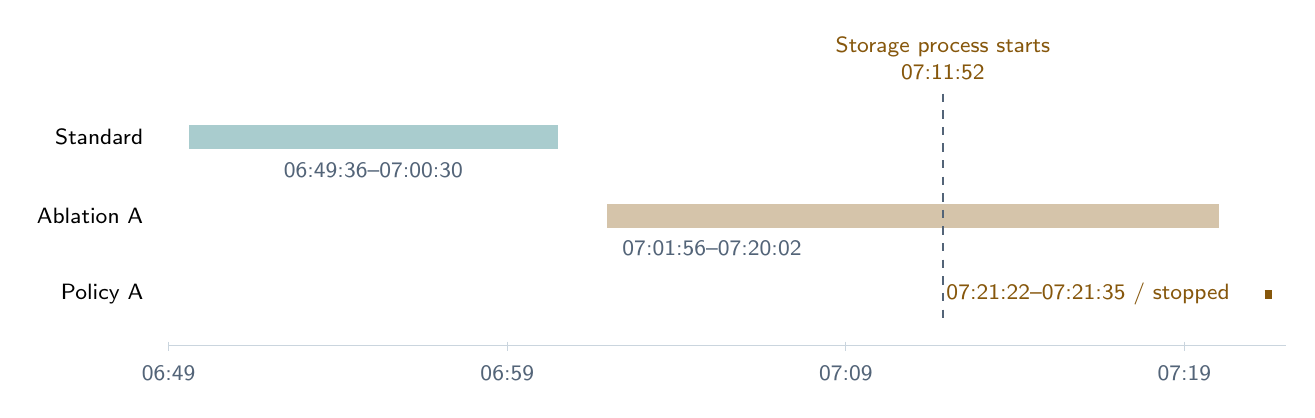
\begin{tikzpicture}[x=1cm,y=1cm,font=\sffamily\fontsize{8.4}{10}\selectfont]
\node[anchor=east] at (2.8,0) {Standard};
\node[anchor=east] at (2.8,-1) {Ablation A};
\node[anchor=east] at (2.8,-2) {Policy A};
\fill[Teal!35] (3.258,-.15) rectangle (7.945,.15);
\fill[Amber!35] (8.5613,-1.15) rectangle (16.3443,-.85);
\draw[Amber,line width=3pt] (16.9177,-2)--(17.0107,-2);
\draw[Muted,dashed,line width=.8pt] (12.8327,.55)--(12.8327,-2.35);
\node[anchor=south,align=center,text=Amber] at (12.8327,.60) {Storage process starts\\07:11:52};
\node[anchor=north,text=Muted] at (5.6,-.2) {06:49:36--07:00:30};
\node[anchor=north,text=Muted] at (9.9,-1.2) {07:01:56--07:20:02};
\node[anchor=east,text=Amber] at (16.6,-2) {07:21:22--07:21:35 / stopped};
\draw[Rule] (3,-2.65)--(17.19,-2.65);
\foreach \x/\lab in {3/06:49,7.3/06:59,11.6/07:09,15.9/07:19} {
 \draw[Rule] (\x,-2.60)--(\x,-2.72);
 \node[anchor=north,text=Muted] at (\x,-2.78) {\lab};
}
\end{tikzpicture}
\end{center}
{\smallbody
A post-ablation snapshot showed storage-management activity above 190\% CPU. This establishes potential overlap, not continuous utilization or a causal explanation for any individual cell. Do not salvage a subset of ablation timings by guessing the interference window. All ablation timing remains exploratory.

Policy A was mistakenly dispatched in the same tool batch as a host check that showed Stata at 162.3\% CPU and two storage processes at 112.2\% and 84.4\%. The owned runner was stopped after 13.326 seconds. This is a preserved failed run, not a solver failure or a completed policy tournament.
}
\sub{Terminal dispositions}
{\smallbody
\begin{tabularx}{\linewidth}{P{0.16\linewidth}P{0.33\linewidth}Y}
\toprule
\textbf{Evidence} & \textbf{Observed result} & \textbf{Permitted conclusion}\\
\midrule
Standard 20 & Exact results in all cells; 18 pass and two inconclusive, seven pairs. & Quiet observations retained; aggregate nonregression is not established.\\
\addlinespace[4pt]
Ablation A & 26 cells collected; three pairs; 18 carried unavailabilities. Host quietness not established. & Scientific checks remain evidence; timings are exploratory and cannot select a policy.\\
\addlinespace[4pt]
Policy A & 58 traced checks and 232 warmup/measured calls pass; three cell summaries saved. & Partial observations only. Completed fourth-cell calls do not constitute a saved fourth summary; interruption occurred during bootstrap. No selection.\\
\addlinespace[4pt]
B and C & Not run or inspected for selection. & No frozen B winner, public activation or C qualification. The declared deployment transition remains unused.\\
\bottomrule
\end{tabularx}
}
\begin{note}\smallbody
\textbf{Original closing decision: no default change.} At this point the frozen stopping rule authorized no retry or continuation, and no recovery proposal had been approved. Johannes subsequently approved bounded recovery and future retries (page 21). That authorization preserves every earlier failure and observation; it requires prospective bounds and repeated-look accounting, not repeated sampling until a pass. Implementation and scientific checks alone do not establish performance adoption.
\end{note}
\anchor{Retained data: \code{bench/results/solver-routing-20261014.json}; policy source SHA-256 begins \code{5a48c8a0}. Host observations, exact artifact hashes, case/tool identities and original summary values are retained. Maintained interpretation: \code{docs/VALIDATION.md}.}
\vfill
{\sffamily\bfseries\fontsize{9.5}{12}\selectfont\color{Teal}ORIGINAL CLOSE: NO POLICY SELECTED OR PROMOTED. RECOVERY ON PAGE 21.}
\end{compactleaf}


% PAGE 21 ---------------------------------------------------------------------
% Authorized terminal recovery status authored by Codex; not GPT Pro code approval.
\newleaf
\begin{compactleaf}
\sect{20 / AUTHORIZED RECOVERY}{All 20 standard cells now pass}
\tagline{Codex update. Original outcomes remain on pages 18--20. This is the standard gate only.}
\begin{note}\smallbody
Johannes authorized bounded retries and Spotlight mitigation. Prospective bounds, host conditions and repeated-look accounting still apply; earlier outcomes, scientific tolerances, models and allowances are unchanged. \textbf{Replacement policy A is ineligible; B/C remain unopened. Public Auto and explicit IT are unchanged.}
\end{note}
\sub{Terminal wide-OLS result: 7 original + 14 confirmation + 42 new = 63 pairs}
{\smallbody
All 86 replacement calls retained exact science/solver signatures, 11:03:08--11:05:34 America/New\_York. The guard recorded 32 snapshots, maximum unrelated aggregate CPU 44.5 points across 24 logical CPUs, no trigger and complete cleanup. No service was paused. Sampled, decayed CPU readings cannot exclude every source of noise.
}
\begin{center}
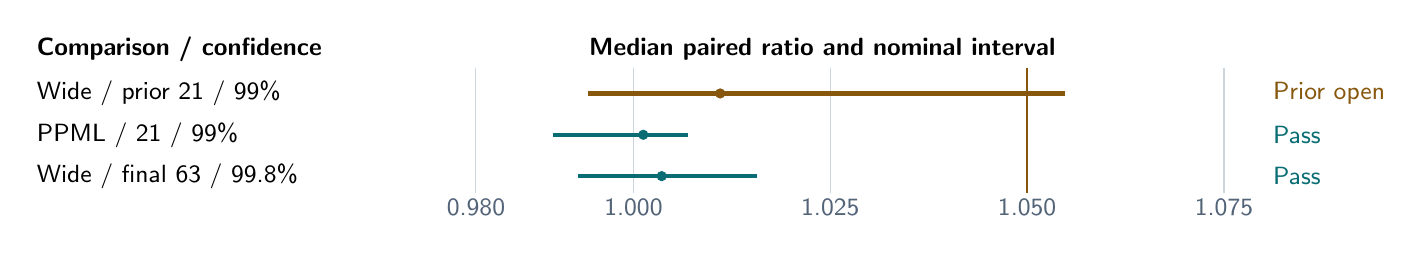
\begin{tikzpicture}[x=1cm,y=0.70cm,font=\sffamily\fontsize{8.7}{10.6}\selectfont]
\node[anchor=west,font=\sffamily\bfseries\fontsize{9}{11}\selectfont] at (0,0.45) {Comparison / confidence};
\node[font=\sffamily\bfseries\fontsize{9}{11}\selectfont] at (10.1,0.45) {Median paired ratio and nominal interval};
\draw[Rule,line width=0.40pt] (5.70000,.12)--(5.70000,-2.15);
\node[text=Muted] at (5.70000,-2.42) {0.980};
\draw[Rule,line width=0.40pt] (7.70000,.12)--(7.70000,-2.15);
\node[text=Muted] at (7.70000,-2.42) {1.000};
\draw[Rule,line width=0.40pt] (10.20000,.12)--(10.20000,-2.15);
\node[text=Muted] at (10.20000,-2.42) {1.025};
\draw[Amber,line width=0.90pt] (12.70000,.12)--(12.70000,-2.15);
\node[text=Muted] at (12.70000,-2.42) {1.050};
\draw[Rule,line width=0.40pt] (15.20000,.12)--(15.20000,-2.15);
\node[text=Muted] at (15.20000,-2.42) {1.075};
\node[anchor=west] at (0,-0.350) {Wide / prior 21 / 99\%};
\draw[Amber,line width=1.5pt] (7.127131,-0.350)--(13.183571,-0.350);
\fill[Amber] (8.801845,-0.350) circle (.065cm);
\node[text=Amber,anchor=west] at (15.7,-0.350) {Prior open};
\node[anchor=west] at (0,-1.100) {PPML / 21 / 99\%};
\draw[Teal,line width=1.5pt] (6.673933,-1.100)--(8.392785,-1.100);
\fill[Teal] (7.825333,-1.100) circle (.065cm);
\node[text=Teal,anchor=west] at (15.7,-1.100) {Pass};
\node[anchor=west] at (0,-1.850) {Wide / final 63 / 99.8\%};
\draw[Teal,line width=1.5pt] (6.994190,-1.850)--(9.263642,-1.850);
\fill[Teal] (8.058862,-1.850) circle (.065cm);
\node[text=Teal,anchor=west] at (15.7,-1.850) {Pass};

\end{tikzpicture}
\end{center}
{\smallbody
\begin{tabularx}{\linewidth}{P{0.29\linewidth}P{0.15\linewidth}Y P{0.13\linewidth}}
\toprule
\textbf{Preserved comparison} & \textbf{Median ratio} & \textbf{Nominal interval} & \textbf{Outcome}\\
\midrule
Wide / prior 21 pairs, 99\% & 1.011018 & [0.994271, 1.054836] & Inconclusive\\
PPML / 21 pairs, 99\% & 1.001253 & [0.989739, 1.006928] & Pass\\
Wide / final 63 pairs, 99.8\% & 1.003589 & [0.992942, 1.015636] & Pass\\
\bottomrule
\end{tabularx}
The final pooled upper endpoint passes 1.05. With the original 18 and PPML passes, \textbf{20/20 standard cells pass}. The new 42 pairs alone are descriptive: median 1.001589, nominal 95\% interval [0.992047, 1.009302]; they do not replace the pooled decision.

The prior confirmation had 60 exact calls in 83.3 seconds, 19 snapshots and maximum unrelated aggregate CPU 50.8. Two attempts remain excluded: eight observations stopped at Core Spotlight 110\% after 20.07 seconds; 40 stopped at 120.6\% after 70.07 seconds. Both were invalidated from host evidence before timing inspection, adding no eligible look.
}
\sub{Frozen terminal rule and confidence limits}
{\smallbody
The terminal continuation preserved artifacts, inputs, median paired-ratio statistic, $\max(5\%,1\ \mathrm{ms})$ allowance and guard: 42 new pairs, one warmup/plugin, 86 calls, 90 seconds/call, 900 seconds total. Analysis uses 10,000 draws, seed 739391 and nominal 99.8\% endpoints 9/9989 (zero-based). A nonpass would have ended collection for this unchanged artifact.

The nominal upper-tail sum is $0.025+0.005+0.001=0.031$, \textbf{not guaranteed 3.1\% sequential error control}. Percentile-bootstrap coverage is approximate; later sample size and confidence were chosen after earlier results, and pooling assumes comparable paired-ratio distributions across sessions. No exact or simultaneous guarantee is claimed.

Policy A: three replacement cohorts were excluded before timing inspection. The first stopped at 60.06 seconds (index store 207.6\% CPU); retry 01 on old-guard FSEvents readings 5.1/5.5\%; retry 02 at 60.07 seconds (index store 110.2\%). Retry 01 retains 164 timing passes, one EPERM block, one unfinished entry and 43 trace passes. A fresh unmeasured diagnostic passed; historical EPERM remains unresolved. Retry 02 retains 512 timing passes, 141 trace passes, one unfinished trace and eight partial summaries.

The guard classifies the inspected FSEvents/WallpaperAerialsExtension paths as ordinary OS/desktop work (25 tests; independent review); Sky remains strict and CPU limits fixed. Retry 03 retains artifacts, cases, grid, statistics and \href{https://developer.apple.com/documentation/xcode/locating-a-missing-debug-symbol-file}{local \code{.noindex} mitigation}. With authorization, the fixed-identity Sky helper was stopped at 19:02:21.710686Z and restored at 19:04:22.631627Z. Admission 06 (19:03:02--19:04:02 UTC) rejected unrelated FEVC Stata validation at 397.3--400.0\% CPU (aggregate 408.4--427.6). No benchmark calls ran; the desktop amendment's two-admission batch is exhausted. A/B/C and activation remain pending; the standard gate and public Auto are unchanged.
}
\anchor{Full outcomes/hashes: \href{VALIDATION.md}{docs/VALIDATION.md}. Retained \href{../bench/results/solver-routing-policy-a-retry01-interrupted-20261014.json}{retry 01} and \href{../bench/results/solver-routing-policy-a-retry02-interrupted-20261014.json}{retry 02 evidence}. Final standard pool \code{2478806f}; prior records remain preserved.}
\vfill
{\sffamily\bfseries\fontsize{9.5}{12}\selectfont\color{Teal}STANDARD GATE PASSED. ROUTING SELECTION PENDING. PUBLIC DEFAULT UNCHANGED.}
\end{compactleaf}

% PAGE 22 ---------------------------------------------------------------------
% Approved prospective measurement method; authored by Codex, not Pro code approval.
\newleaf
\begin{compactleaf}
\renewcommand{\smallbody}{\fontsize{9.2}{10.6}\selectfont\color{Ink}\RaggedRight}
\setlength{\parskip}{1pt}
\setlength{\topsep}{1pt}
\setlength{\abovedisplayskip}{5pt}
\setlength{\belowdisplayskip}{5pt}
\sect{21 / PROSPECTIVE MEASUREMENT}{Controlled blocks, separate decisions}
\tagline{SCC discovery and Mac science pass; the fixed B12 campaign cannot qualify a policy.}
\begin{note}\smallbody
Scientific, resource and transaction gates are unchanged. This method replaces strict CPU admission and whole-panel aborts prospectively. All seven failed admissions and earlier failed/excluded attempts remain historical and unpooled.
\end{note}
\begin{center}
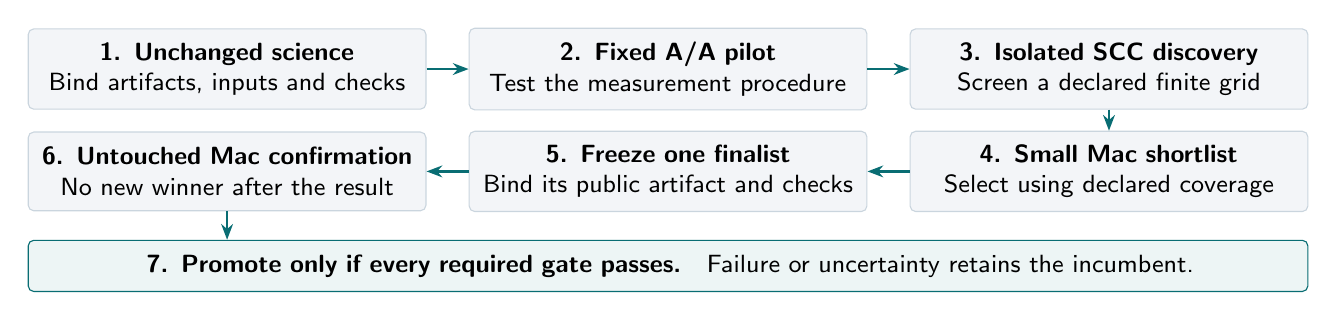
\begin{tikzpicture}[font=\sffamily\fontsize{9}{11}\selectfont,
  stage/.style={draw=Rule,fill=Light,rounded corners=2pt,text width=4.7cm,minimum height=1.0cm,align=center,inner sep=5pt},
  route/.style={-{Stealth[length=2mm]},draw=Teal,line width=.85pt}]
\node[stage] (science) at (0,0) {\textbf{1. Unchanged science}\\Bind artifacts, inputs and checks};
\node[stage] (pilot) at (5.6,0) {\textbf{2. Fixed A/A pilot}\\Test the measurement procedure};
\node[stage] (scc) at (11.2,0) {\textbf{3. Isolated SCC discovery}\\Screen a declared finite grid};
\node[stage] (mac) at (11.2,-1.3) {\textbf{4. Small Mac shortlist}\\Select using declared coverage};
\node[stage] (freeze) at (5.6,-1.3) {\textbf{5. Freeze one finalist}\\Bind its public artifact and checks};
\node[stage] (confirm) at (0,-1.3) {\textbf{6. Untouched Mac confirmation}\\No new winner after the result};
\node[stage,fill=Pale,draw=Teal,text width=15.9cm,minimum height=.65cm] (decision) at (5.6,-2.5) {\textbf{7. Promote only if every required gate passes.}\quad Failure or uncertainty retains the incumbent.};
\draw[route] (science)--(pilot); \draw[route] (pilot)--(scc);
\draw[route] (scc)--(mac); \draw[route] (mac)--(freeze);
\draw[route] (freeze)--(confirm); \draw[route] (confirm.south)--(confirm.south |- decision.north);
\end{tikzpicture}
\end{center}
\sub{Complete solves and the tested quantity}
{\smallbody
Use complete balanced randomized ABBA/BAAB solves, including setup (A: reference; B: candidate label). In seconds, $B_j=\sqrt{t_{A1}t_{A2}}$ and $N_j=\sqrt{t_{B1}t_{B2}}$; test $E_j=N_j-B_j-\max(0.05B_j,0.001)$.
The median of $N_j/B_j$ is a separate descriptive effect size. It is not the acceptance statistic; minima cannot pass the gate. Sort scores $E_{(1)}\le\cdots\le E_{(n)}$. With $\alpha=0.025$, take the smallest attainable rank $k$ satisfying
\[
 \Pr\{\operatorname{Binomial}(n,\tfrac12)\ge k\}\le0.025,\qquad U=E_{(k)}.
\]
Pass only when $U\le0$, retaining ties. No attainable rank means $U=+\infty$ and an inconclusive result. Coverage is conditional on independent block scores with a common median. A small A/A pilot can reveal order effects or dependence; it cannot prove independence or common medians.
}
\sub{Freeze budgets; distinguish noise from invalidation}
{\smallbody
Before collection freeze artifacts, inputs, workers, warmups, cache policy, order seed, block/attempt/wall budgets, round/session identities and analysis unit. Shuffle workloads by round; checkpoint complete blocks. Discovery may use declared balanced rotation. Preserve pairing and shared-reference correlations; correlated solves are not independent observations.

Record ordinary OS bursts as noise. Known competing compute or host faults invalidate whole affected blocks only through frozen rules and external evidence, never through unfavorable timings. Retain incomplete/excluded blocks and cap replacements prospectively. Science failures and solver timeouts keep their failure semantics; \textbf{the allowance remains $\max(5\%,1\ \mathrm{ms})$}. No fallback winner or sampling until success follows confirmation.
}
\sub{Host scope and current boundary}
{\smallbody
SCC comparisons need verified node isolation and fixed CPU/thread placement; slots alone are insufficient. Linux does not establish Mac speed.

The A/A pilot passed 72 conditional blocks, with serial dependence unresolved. The full suite and 330 benchmark tests pass; production is unchanged across 192 runtime modules and 58 artifact inputs.

Linux discovery passed science, final accounting and strict isolation after certified recovery; failed rounds and attempts remain excluded. Astra reproduced 13 rankings from 7,614 values; the shortlist was baseline, h32-k0, h16-k0 and h32-k1.

Mac science admits 42 cells: 468 passing requests and 18 unchanged optional unavailabilities. Reviewed checker corrections and eight missing repeats preserve model bytes and full first-call fingerprints. No first call or unavailable arm was retried; Linux availability was not imported.

The fixed B12 collection completed all 504 blocks and 11,700 calls, with passing contemporary science checks, in 8,477.926 seconds excluding preflight. However, padded macOS executable names caused the frozen observer classifier to miss known computation. Independent review checks 2,555 retained snapshots and 3,298,909 process rows. Normalizing only name padding under the same rules identifies 102 affected blocks. One cell retains four blocks: $2^{-4}>0.025$, so its upper median bound is not finite.

Both descriptive audits reject all four frontiers; the faulty all-block mask has 43, 47, 53 and 53 failed edges. \textbf{No policy qualifies; no promotion or C access follows. Public Auto is unchanged.} Original failures, parsed snapshots and source-bound fingerprints remain preserved. Original \code{ps} stdout and successful timed numeric outputs are unavailable. Next: prospective observer repair and materially revised routing with new qualification, not current-policy resampling.
}
\anchor{\href{development_workflow.md}{Approved protocol} (\code{da8551cc}); \href{../bench/results/solver-routing-controlled-20261014.json}{controlled evidence}; \href{VALIDATION.md}{validation}. Codex-authored amendment.}

\end{compactleaf}

% PAGES 23+ / source-reviewed private portfolio; no qualification claim.
\newleaf
\fancyhead[R]{\sffamily\fontsize{8.5}{10}\selectfont\color{Muted}AMENDMENT / 15 OCTOBER 2026}
\fancyfoot[L]{\sffamily\fontsize{8}{10}\selectfont\color{Muted}Private portfolio / qualification pending}
\begin{compactleaf}
\smallbody
\sect{PROSPECTIVE AMENDMENT / 1 OF 4}{One fixed portfolio, three structural paths}
\tagline{Implemented private qualification arm: \code{routing\_portfolio\_v1}. Public Auto remains unchanged.}
\begin{note}\smallbody
\textbf{Status.} This amendment describes the private implementation. Its fixed 92-call development study passed all independent scientific checks and all 46 exact repeats. Declared route coverage remains incomplete; performance qualification is pending. It neither selects a winner nor reopens the closed Mac B NO-GO; old C remains untouched.
\end{note}
\begin{center}
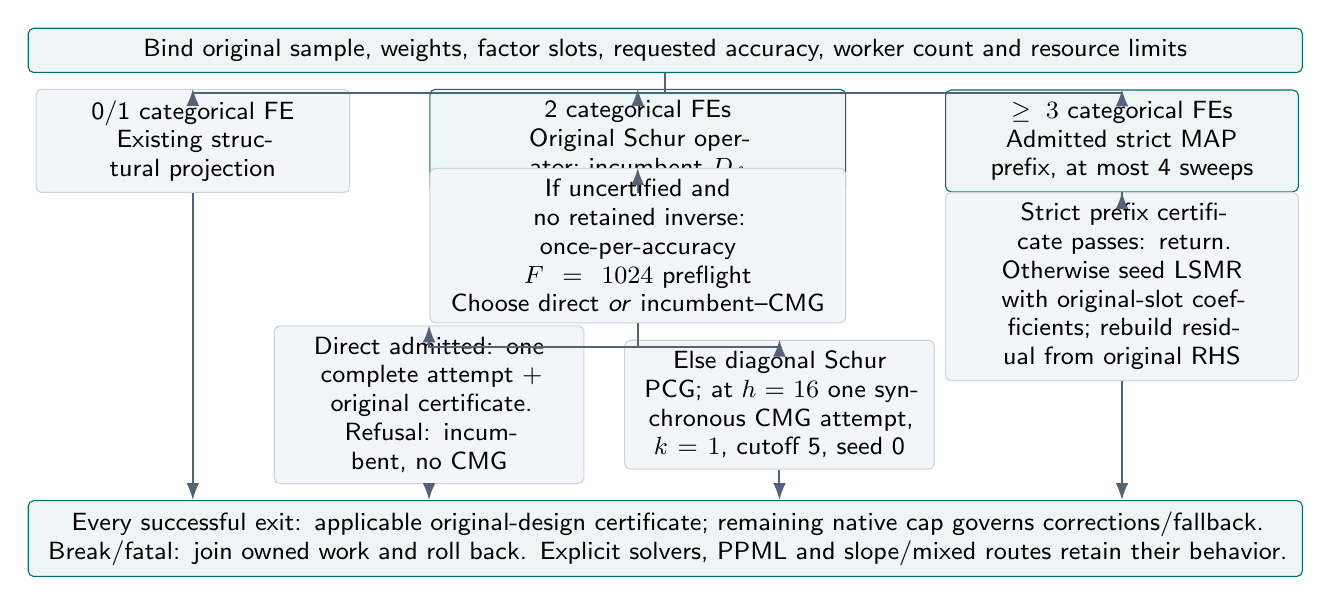
\begin{tikzpicture}[x=1cm,y=1cm,>=Latex,
 box/.style={draw=Rule,fill=Light,rounded corners=2pt,align=center,font=\sffamily\fontsize{8.6}{10.4}\selectfont,inner sep=4pt},
 focus/.style={box,draw=Teal,fill=Pale},
 arr/.style={->,line width=.7pt,draw=Muted},
 lab/.style={font=\sffamily\fontsize{8}{9.5}\selectfont,fill=white,inner sep=1.5pt,text=Muted}]
\node[focus,text width=15.9cm] (start) at (8.2,0) {Bind original sample, weights, factor slots, requested accuracy, worker count and resource limits};
\node[box,text width=3.7cm] (exact) at (2.2,-1.15) {0/1 categorical FE\\Existing structural projection};
\node[focus,text width=5.0cm] (two) at (7.85,-1.15) {2 categorical FEs\\Original Schur operator; incumbent $D_f$};
\node[focus,text width=4.2cm] (many) at (14.0,-1.15) {$\geq3$ categorical FEs\\Admitted strict MAP prefix, at most 4 sweeps};
\node[box,text width=5.0cm] (choose) at (7.85,-2.48) {If uncertified and no retained inverse:\\once-per-accuracy $F=1024$ preflight\\Choose direct \emph{or} incumbent--CMG};
\node[box,text width=4.2cm] (seed) at (14.0,-3.00) {Strict prefix certificate passes: return.\\Otherwise seed LSMR with original-slot coefficients; rebuild residual from original RHS};
\node[box,text width=3.65cm] (direct) at (5.2,-4.5) {Direct admitted: one complete attempt + original certificate.\\Refusal: incumbent, no CMG};
\node[box,text width=3.65cm] (cmg) at (9.65,-4.5) {Else diagonal Schur PCG; at $h=16$ one synchronous CMG attempt, $k=1$, cutoff 5, seed 0};
\node[focus,text width=15.9cm] (finish) at (8.2,-6.2) {Every successful exit: applicable original-design certificate; remaining native cap governs corrections/fallback.\\Break/fatal: join owned work and roll back. Explicit solvers, PPML and slope/mixed routes retain their behavior.};
\draw[arr] (start.south) -- ++(0,-.25) -| (exact.north);
\draw[arr] (start.south) -- ++(0,-.25) -| (two.north);
\draw[arr] (start.south) -- ++(0,-.25) -| (many.north);
\draw[arr] (two)--(choose);
\draw[arr] (choose.south)--++(0,-.3)-|(direct.north);
\draw[arr] (choose.south)--++(0,-.3)-|(cmg.north);
\draw[arr] (many)--(seed);
\draw[arr] (exact.south)--(2.2,-5.6)--(finish.north -| exact.south);
\draw[arr] (direct.south)--(finish.north -| direct.south);
\draw[arr] (cmg.south)--(finish.north -| cmg.south);
\draw[arr] (seed.south)--(finish.north -| seed.south);
\end{tikzpicture}
\end{center}
\vspace{-4pt}
\begin{tabularx}{\linewidth}{P{.14\linewidth}P{.31\linewidth}Y}
\toprule
\textbf{Geometry} & \textbf{Intended frontier} & \textbf{Cost and limitation}\\
\midrule
0/1 FE & Preserve existing cheap projection. & No optional profiling benefit; other estimation costs may dominate.\\
2 FEs & Direct for fully admitted small retained systems; incumbent for easy graphs; sampled CMG for unresolved modes. & Direct factors and RHS work can dominate; a small year dimension alone does not imply admission. CMG setup/application may lose to cheap iterations.\\
$\geq3$ FEs & MAP can finish easy systems; an unfinished prefix provides a coefficient seed. & Prefix copies, sweeps and certificates are overhead on hard systems. It replaces the old shortcut; there is \emph{no general-pair CMG checkpoint} in V1.\\
\bottomrule
\end{tabularx}
\sub{The same problem, a finite hypothesis}
For two FEs, $S=D_f-B^{\mathsf T}D_w^{-1}B$ remains the exact implicit Schur operator. One connected weighted tree per above-cutoff worker changes only the fixed preconditioner; low-degree cliques stay exact. Connectivity and unbiasedness do not give a universal spectral or runtime guarantee. Original sample, rank, omissions, factor slots and both bias modes remain authoritative. No family labels, seed search or new $h/k$ grid select this arm.
\anchor{\code{docs/SPEC.md}; core \code{fe/routing.rs} and \code{fe/borrowed\_map.rs};\newline categorical-prefix implementation under \code{fe/borrowed\_map/}. Paths beneath \code{crates/fereg-core/src/}.}

\newpage
\smallbody
\sect{PROSPECTIVE AMENDMENT / 2 OF 4}{Charged bounds, memory and evidence}
\tagline{Work units are conservative operation/access charges, not seconds or predictions of speed.}
\sub{Two separate work tests; no certificate credit for optional preparation}
For $n$ observations, incumbent orientation sizes $p,q$, $r$ active RHSs and physical bank stride $s$, the checked Schur tariff is
\[
 W(n,p,q,r,s)=10nr+10n+(4p+64q)r+(p+3q)s+8p+12q+64r.
\]
$W_0$ fixes the physical setup reference at the first active batch. $W_{\rm ref}=W(n,p,q,r,r)$ prices the current packed RHSs without inactive-bank credit. Let $U$ be already spent setup work \emph{before} the direct preflight, $F=1024$, $A$ the subsequent noncertificate direct work, and $C$ its original-design certificate:
\[
 \boxed{F+A\leq4W_{\rm ref}},\qquad
 \boxed{A+C\leq32W_0-U-F}.
\]
For a fully admitted attempt, returned work is $A+C$, excluding already charged $F$. Census/profile refusals return their incurred prefix work, without charging an unrun certificate. Census, \emph{both} orientation profiles, assembly, factorization, current-RHS solves, reconstruction and direct-only checks belong to $A$. The complete admitted reservation is charged before numerical work, even if a later test refuses it. Protected fallback/output reserves and joint memory admission still apply.

Keep the incumbent orientation fixed in $W_{\rm ref}$. For each candidate eliminated/retained orientation, use $L=p+q$, $c=\min(p,q)$, $z=q-1$ and $J=\min\{pqz/2,\lfloor nz/2\rfloor\}$, its sufficient bound is
\[
\begin{aligned}
 A_{\rm ub}={}&(13+g)n+hnr+72L+64c+18Lr+128\\
             &+32z^2(q+r)+48J,
\end{aligned}
\]
where $(g,h)=(18,36)$ for unit weights and $(34,52)$ for provided weights. The original two-FE certificate is bounded by
\[
 C=152nr+112n+128r+64\lceil n/512\rceil r+128Lr.
\]
Use $A_{\rm ub}$ in both admission tests and check complete joint memory before scanning. Any admitted bound opens the direct attempt; its preflight profile is discarded. The subsequent census profiles both actual orientations and selects the least admitted complete work, with original effect order breaking ties. Component-square and cubic sums are bounded by $(q-1)^2$ and $(q-1)^2q$; $J$ bounds clique pairs. Overflow declines; conservative bounds can reject a feasible solve.

Only a request without a retained inverse runs this preflight. A selected direct attempt consumes its one opportunity for that accuracy key. On preflight decline, its charge remains and one CMG opportunity survives across Low chunks. Chunks never replenish setup quota. A new accuracy/final-residual key has its own allowance and may reuse a retained CMG inverse.

\sub{CMG construction and canonical cache}
At the fixed unresolved checkpoint, CMG must fit the remaining $32W_0$ ledger, its $4W_0$ handoff reserve, startup application charge and joint memory envelope. Installation uses a fresh original-operator correction residual; refusal preserves the incumbent recurrence. The synchronous cache saves first-pass canonical cells, offsets and compensated totals, preserving emission/sampler order and bits. Before allocation, one checked envelope covers cache, cell/sampler scratch, graph, components, hierarchy and scalar/application banks alongside live parent storage. Insufficient memory or overflow selects the original two-pass path \emph{before} allocation. Its separate 1,024-unit cache-admission charge, stores and reads remain charged; cache storage is reserved through finish, with no ledger refund.

\sub{Strict many-FE continuation; parallel preparation is a separate option}
For each action request $\tau$ (final residual: $\min(\tau,10^{-14})$), prefix, seeded correction and MAP fallback use
$\tau_* = \tau$ if $\tau\leq10^{-14}$, otherwise $\max(10^{-2}\tau,10^{-14})$.
An accepted prefix may require its existing confirmation sweep, still within four. Admission may skip it; actual sweeps consume the unchanged action cap. Original RHS, weights, normalization and factor-slot seed are preserved.

V1 builds CMG synchronously. Existing \code{routing\_overlap\_*} arms instead reserve one scoped worker, retain fixed foreground partitions on at most $P-1$ executing workers, and issue bounded deterministic grants. This can hide preparation but costs a core and simultaneous live memory; refusal, cancellation and join rules remain binding. It is not activated here, and no unmeasured overlap or batching gain is claimed.

\newpage
\smallbody
\sect{PROSPECTIVE AMENDMENT / 3 OF 4}{Development proof and the next gate}
\tagline{Scientific checks pass; incomplete route coverage and construction refusals remain visible.}
\sub{Canonical preparation is a large share of charged construction work}
\begin{center}
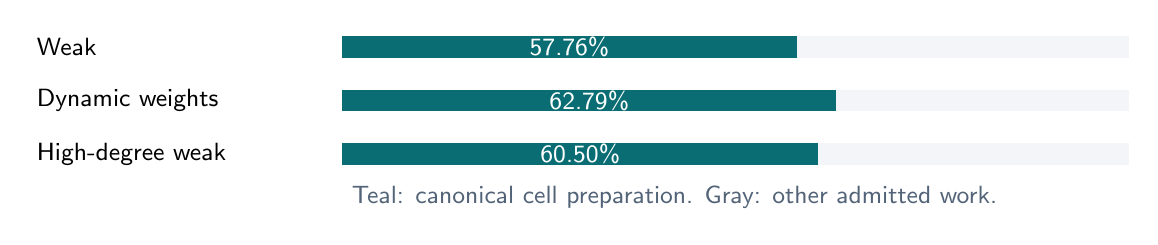
\begin{tikzpicture}[x=1cm,y=.68cm,font=\sffamily\fontsize{9}{11}\selectfont]
\foreach \y/\label/\share/\pct in {0/Weak/5.77624/57.76,-1/Dynamic weights/6.27870/62.79,-2/High-degree weak/6.04995/60.50}{
 \node[anchor=west] at (0,\y) {\label};
 \fill[Light] (4,\y-.2) rectangle (14,\y+.2);
 \fill[Teal] (4,\y-.2) rectangle ({4+\share},\y+.2);
 \node[text=white] at ({4+\share/2},\y) {\pct\%};
}
\node[anchor=west,text=Muted] at (4,-2.8) {Teal: canonical cell preparation. Gray: other admitted work.};
\end{tikzpicture}
\end{center}
\vspace{-3pt}
\begin{binding}\tinybody
\textbf{Evidence and next gate.} The 40-call diagnostic committed in \code{377226f8} passed its independent science and exact repeats. Cell load/sort/aggregation comprised \textbf{57.76\%, 62.79\%, 60.50\%} of admitted work for weak, dynamic-weight and high-degree weak primary builds: \emph{work shares, not speedups}. Refusal can occur later; saving those passes does not prove build completion. Same-hierarchy scalar/batch witnesses were exact. The initial V1 92-call study observes certified direct solves at one/four workers, seeded LSMR and high-degree CMG installation. Weak CMG exhausts its builder allowance; weighted and wide-RHS solves finish before iteration 16. That 92-call study does not attest early-prefix acceptance or cache admission. No extra calls repair its missing route coverage. The failed old B supplies no promotion or reused shortlist.

The prospective SCC discovery uses three distinct isolated hosts/jobs, each a full fresh 42-cell round: two science calls plus one traced prerequisite, one warmup and three measured calls per case--arm slot; at most $3\times360\times7=7560$ calls. Caps: 120 s/call, 14,400 s/allocation, 43,200 allocation-seconds total; no replacements or partial rescue. All three valid rounds precede the frozen descriptive rejection screen. Only a surviving fixed candidate may enter separately frozen fresh Mac B and untouched C, against the qualified incumbent with matched release profiles. No universal runtime guarantee follows from this design.
\end{binding}
\sub{S1 route coverage: 92 checks and 46 exact repeats}
\begin{tabularx}{\linewidth}{P{.23\linewidth}P{.34\linewidth}Y}
\toprule
\textbf{Path} & \textbf{Observed at one/four workers} & \textbf{Remaining limitation}\\
\midrule
Many-FE prefix & All three cases continue through seeded LSMR. & No early-prefix certificate observed.\\
Weak CMG & Both action attempts refuse with cumulative setup just below $28W_0$. & The diagnostic pair locates terminal sparse numeric refusal.\\
High-degree CMG & Primary hierarchy installs; primary/final counts 22/8 versus old 53/27. & Iteration reduction does not establish a speedup.\\
Weighted / wide RHS & Counts 7/6 and 14/13; neither reaches checkpoint 16. & No CMG construction required on these inputs.\\
Small direct system & Both action certificates pass with zero iterations. & One declared development model; no general runtime claim.\\
\bottomrule
\end{tabularx}
\vspace{3pt}
\smallbody
The six-call attribution stopped at call five because seeded-session timers covered the wrong entry path. The protocol remains failed, with no sixth call or retry. All five saved results pass offline science/reference checks; the first four form two verified diagnostic pairs. They confirm cache admission and no emission reloads. The weak 500-vertex graph triggers the upstream 700 direct threshold and exhausts work in its 499-unknown sparse factorization. Further engineering must preserve allowances and fallback reserves; no performance or completed-probe claim follows.
\anchor{\code{fe/routing.rs}, \code{fe/routing\_direct.rs}, \code{fe/cmg\_schur/bounded.rs};\newline \code{bench/routing\_parallel.py}; maintained evidence in \code{docs/VALIDATION.md}.}


% PAGE 26 / approved factor-affordability screen; final functional study passes.
\newpage
\smallbody
\sect{PROSPECTIVE AMENDMENT / 4 OF 4}{Terminal factor affordability}
\tagline{One private-portfolio opt-in; unchanged thresholds, work tariff and hard allowances.}
\begin{note}[top=4pt,bottom=4pt,before skip=4pt,after skip=4pt]\smallbody
\textbf{Purpose.} Screen a prospective direct terminal against a conservative integer work bound. This is neither reserved credit nor a guarantee of completion, installation, convergence or speed.
\end{note}
\begin{center}
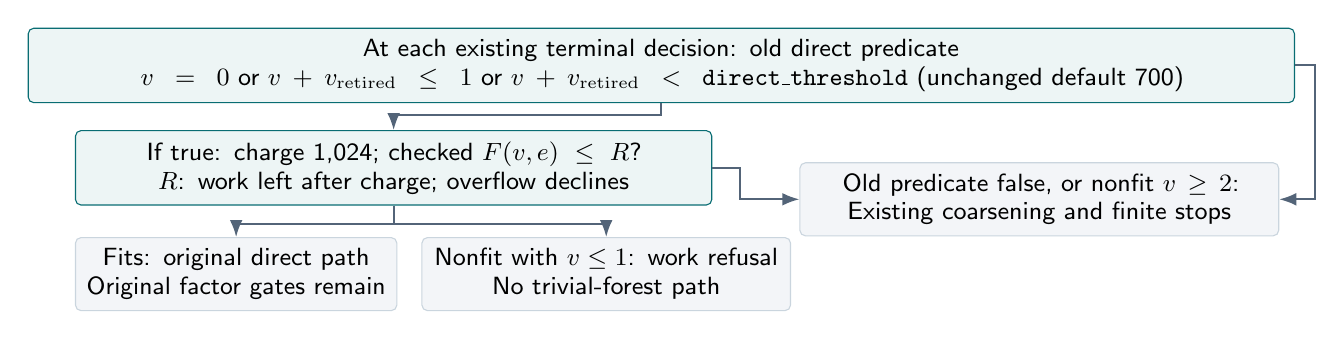
\begin{tikzpicture}[x=1cm,y=1cm,>=Latex,
 box/.style={draw=Rule,fill=Light,rounded corners=2pt,align=center,font=\sffamily\fontsize{8.6}{10.4}\selectfont,inner sep=4pt},
 focus/.style={box,draw=Teal,fill=Pale},
 arr/.style={->,line width=.7pt,draw=Muted},
 lab/.style={font=\sffamily\fontsize{8}{9.5}\selectfont,fill=white,inner sep=1.5pt,text=Muted}]
\node[focus,text width=15.8cm] (old) at (8.2,0) {At each existing terminal decision: old direct predicate\\$v=0$ or $v+v_{\rm retired}\leq1$ or $v+v_{\rm retired}<\texttt{direct\_threshold}$ (unchanged default 700)};
\node[focus,text width=7.8cm] (check) at (4.8,-1.3) {If true: charge 1,024; checked $F(v,e)\leq R$?\\$R$: work left after charge; overflow declines};
\node[box,text width=5.8cm] (coarse) at (13.0,-1.7) {Old predicate false, or nonfit $v\geq2$:\\Existing coarsening and finite stops};
\node[box,text width=3.8cm] (factor) at (2.8,-2.65) {Fits: original direct path\\Original factor gates remain};
\node[box,text width=4.4cm] (refuse) at (7.5,-2.65) {Nonfit with $v\leq1$: work refusal\\No trivial-forest path};
\draw[arr] (old.south)--++(0,-.15)-|(check.north);
\draw[arr] (old.east)--++(.25,0)|-(coarse.east);
\draw[arr] (check.east)--++(.35,0)|-(coarse.west);
\draw[arr] (check.south)--++(0,-.23)-|(factor.north);
\draw[arr] (check.south)--++(0,-.23)-|(refuse.north);
\end{tikzpicture}
\end{center}
\vspace{-5pt}
\sub{Exact dimension-only charge bounds}
Let $v,e$ count terminal vertices and canonical undirected edges; $v$ is not observation count $n$. Define $d=\max(v-1,0)$, $T=\binom d2$, $U=\binom d3$ (zero below their order), and $H(d)=\lfloor\log_2\max(d,1)\rfloor+1$. These local $F,C$ denote factor/discovery work, not page 24's preflight/certificate.
\[
\begin{aligned}
 C(v,e)&=64+112v+80e+24\binom v2,\\
 S(d)&=16+16\max(d-1,0)+64\bigl(\lfloor d/2\rfloor+\max(d-1,0)\bigr)H(d),\\
 F(v,e)&=456+C(v,e)+936v+968d+784e\\
       &\quad+680T+128U+S(d).
\end{aligned}
\]
$C$ bounds compression paths by $2e+v+\binom v2$ using strictly decreasing parents; $S$ includes final heapsort sift loops. $F$ covers the complete component factor, packed cross-component zero slots and conversion. Checked \code{u128} arithmetic/conversion declines on overflow; integer leading-zero arithmetic computes $H$. Preflight scans no graph and performs no symbolic factorization.

\sub{Resources, scope and tradeoffs}
The enabled entrypoint requires component-terminal factorization. Its meter shadows the caller's finite post-admission remainder; callbacks alone debit the caller. Each screened direct decision pays 1,024. One hierarchy is built: no failed-factor retry, second setup or forced endpoint.

\begin{tabularx}{\linewidth}{P{.25\linewidth}Y}
\toprule
\textbf{Choice or cost} & \textbf{Binding limitation}\\
\midrule
Conservative cubic bound & May reject an affordable sparse factor. Further coarsening changes hierarchy, rounding and iterations without promising improvement.\\
Original later obligations & Reporting, scans, centering, factor, workspace and startup gates can still refuse. The $32W_0$ cap and $4W_0$ handoff reserve remain unchanged.\\
Existing finite stops & Stagnation, fill and maximum levels remain binding; the existing diagonal terminal may be weak. Direct refusal does not force installation.\\
\bottomrule
\end{tabularx}
\begin{binding}\tinybody
\textbf{Scope and evidence.} Only the private portfolio opts in; public Auto, explicit/default builders and existing controlled, reduced and overlap routes remain unchanged. Original operators, tolerances, model decisions, Break/refusal and one-attempt accounting stay binding.

Published CMG \code{3422b04} passes 115 default and 220 all-feature tests, strict Clippy and formatting. Fereg passes 46 focused checks, strict core Clippy and the full test entrypoint. The final universal eight-call study passes independent science, four exact repeat pairs, cross-worker decisions and resource checks; weak and high-degree weak CMG install at iteration 16 with one/four workers. Twelve compatible-dipole cases do \emph{not} certify all-RHS floating-point stability. Earlier rounded-matvec failures remain explicit. No speed, default activation or performance qualification follows.
\end{binding}
\anchor{Design \code{bb93342e}; CMG \code{3422b04}; fereg \code{3f487f21}; upstream \code{hierarchy.rs}, \code{ldl.rs}, \code{preconditioner.rs}; fereg \code{bounded.rs::finish}.}

% PAGE 27 / completed fresh portfolio discovery; no Mac selection or promotion.
\newpage
\fancyhead[R]{\sffamily\fontsize{8.5}{10}\selectfont\color{Muted}EVIDENCE / 16 OCTOBER 2026}
\fancyfoot[L]{\sffamily\fontsize{8}{10}\selectfont\color{Muted}Private portfolio / discovery NO-GO}
\smallbody
\sect{EVIDENCE UPDATE / 16 OCTOBER}{Targeted gains; portfolio NO-GO}
\tagline{Three complete Linux rounds. Descriptive discovery ratios; no Mac performance claim.}
\begin{center}
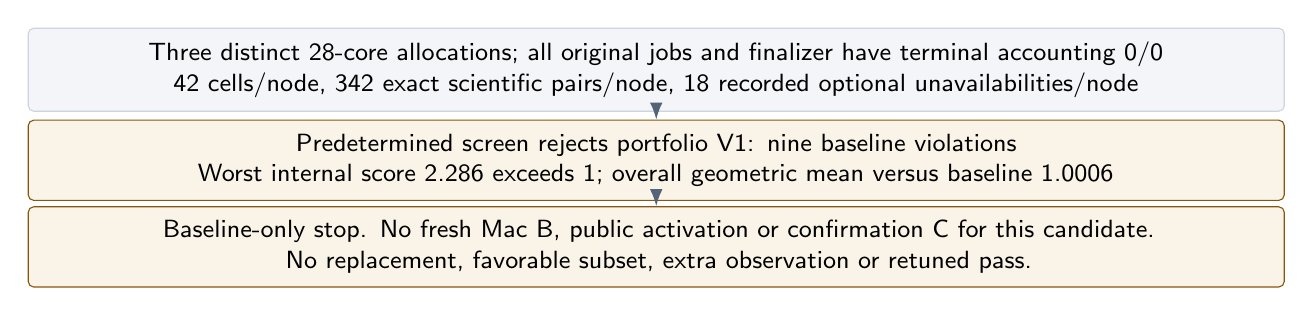
\begin{tikzpicture}[x=1cm,y=1cm,>=Latex,
 box/.style={draw=Rule,fill=Light,rounded corners=2pt,align=center,font=\sffamily\fontsize{9}{11}\selectfont,inner sep=5pt},
 stop/.style={box,draw=Amber,fill=Warm},arr/.style={->,line width=.7pt,draw=Muted}]
\node[box,text width=15.6cm] (run) at (8.2,0) {Three distinct 28-core allocations; all original jobs and finalizer have terminal accounting 0/0\\42 cells/node, 342 exact scientific pairs/node, 18 recorded optional unavailabilities/node};
\node[stop,text width=15.6cm] (screen) at (8.2,-1.15) {Predetermined screen rejects portfolio V1: nine baseline violations\\Worst internal score 2.286 exceeds 1; overall geometric mean versus baseline 1.0006};
\node[stop,text width=15.6cm] (close) at (8.2,-2.25) {Baseline-only stop. No fresh Mac B, public activation or confirmation C for this candidate.\\No replacement, favorable subset, extra observation or retuned pass.};
\draw[arr] (run)--(screen);\draw[arr] (screen)--(close);
\end{tikzpicture}
\end{center}
\vspace{-5pt}
\sub{Complete-solve portfolio / baseline ratios}
For each cell: median of nine within-node paired ratios, using three measured slots per node. Values below 1 are faster. Nodes and slots are not nine independent statistical units; these point estimates carry no Mac qualification interval. The full-precision screen retains max(5\%, 1 ms) against baseline and max(20\%, 1 ms) against every available internal comparator.
\begin{center}
\begin{tabular}{lrr}
\toprule
\textbf{Family} & \textbf{1 worker} & \textbf{4 workers}\\
\midrule
Weak two-FE & \textcolor{Teal}{0.669} & 1.010\\
High-degree weak & \textcolor{Teal}{0.773} & \textcolor{Amber}{1.122}\\
Dynamic weights & \textcolor{Teal}{0.654} & 0.950\\
Small third FE & \textcolor{Amber}{1.108} & 0.994\\
Four FEs & \textcolor{Amber}{1.066} & 0.986\\
Eight FEs & \textcolor{Amber}{1.075} & \textcolor{Amber}{1.073}\\
Sixteen FEs & \textcolor{Amber}{1.112} & \textcolor{Amber}{1.310}\\
Near-confounded third FE & \textcolor{Amber}{1.333} & \textcolor{Amber}{1.122}\\
Wide RHS & 1.001 & 0.999\\
\bottomrule
\end{tabular}
\end{center}
\vspace{-5pt}
\sub{What the result establishes and what remains open}
One-worker difficult two-FE inputs show approximately 23--35\% lower times, but those gains mostly disappear at four workers. Eight of nine baseline violations involve at least three FEs. The overall ratio near 1 combines gains and losses; it does not establish neutrality. The worst internal edge is sixteen FEs/four workers versus LSMR: ratio 1.457 at allowance 1.20. Its normalized score $(1.45712656-1)/0.20\approx2.286$ is not a 2.286-fold runtime.

The complete strict-prefix/seeded-LSMR path needs attribution; these comparisons do not isolate the cost of MAP sweeps. Serial bounded CMG setup/application, hierarchy quality, checkpoint delay and certification are separate possible causes of the four-worker result. Existing wide-RHS parity supplies no evidence for always building earlier on wide batches.

\begin{binding}\tinybody
\textbf{RHS limitation.} The hierarchy is shared, but V1 applies scalar CMG cycles. Its setup allowance scales with the first nontrivial batch and physical storage width; activation remains at iteration 16. Low mode normally starts with the outcome alone, then reuses that allowance across regressor chunks. There is no explicit remaining-RHS payback test. Any successor must price actual compatible remaining work, including setup, handoff, applications and certificates, under a separately declared design.

\textbf{Evidence boundary.} Independent Astra high review passes the retained records, proofs and complete ranking. Pure replay job \code{8140245} passes 0/0 with no native calls and reproduces the entire canonical aggregate. Raw isolation replay checks 4,712 process snapshots and 794 successful scheduler commands, with no detected competing compute. Successful numerical arrays were deleted by the frozen producer: their oracle/scoped checks are source-bound producer attestations, not a fresh recomputation from missing arrays. All failures remain recorded; the old Mac B is still closed. No new full GPT Pro review is claimed.
\end{binding}
\anchor{SCC source \code{cc2aae4d}; jobs \code{8137670--8137673}; canonical aggregate \code{a89d5000}. Full comparison and accounting summaries: \code{docs/VALIDATION.md} and \code{bench/results/solver-routing-controlled-20261014.json}.}
\clearpage

% PAGE 28 / completed observational attribution; prospective causal comparison.
\fancyfoot[L]{\sffamily\fontsize{8}{10}\selectfont\color{Muted}Private portfolio / engineering diagnosis only}
\smallbody
\sect{COST DIAGNOSIS / 16 OCTOBER}{Construction and prefixes dominate}
\tagline{48 fixed calls, six revealed discovery families, one/four workers. No new qualification.}
The instrumented build changes clocks and logging only. All 36 comparisons against the first result in each of 12 cells preserve scientific results, column fingerprints and solver signatures exactly. Below are medians of \emph{two instrumented observations}; ordinary desktop activity and measurement overhead remain. These are inclusive elapsed phases, not CPU shares or estimates of achievable speedup.

\sub{Four-worker cost breakdown, milliseconds}
\begin{center}
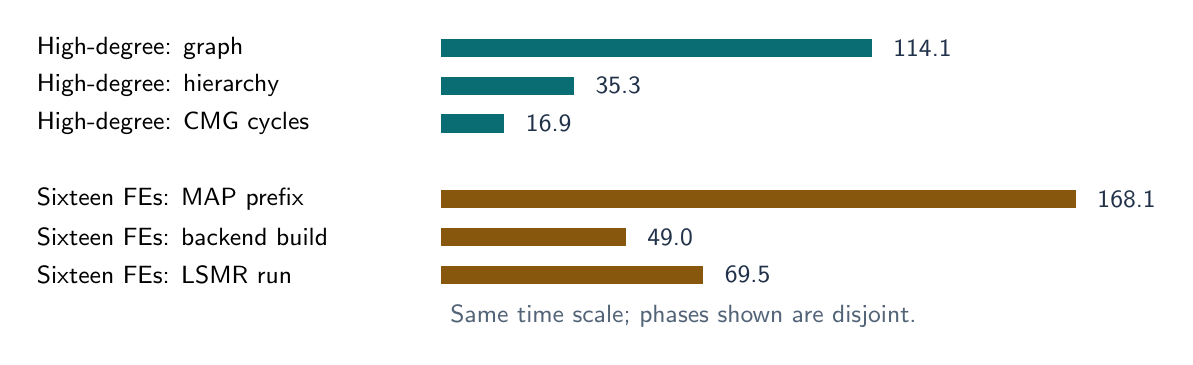
\begin{tikzpicture}[x=1cm,y=.48cm,font=\sffamily\fontsize{8.6}{10.5}\selectfont]
\foreach \y/\label/\value/\shade in {0/High-degree: graph/114.1/Teal,-1/High-degree: hierarchy/35.3/Teal,-2/High-degree: CMG cycles/16.9/Teal,-4/Sixteen FEs: MAP prefix/168.1/Amber,-5/Sixteen FEs: backend build/49.0/Amber,-6/Sixteen FEs: LSMR run/69.5/Amber}{
 \node[anchor=west] at (0,\y) {\label};
 \fill[\shade] (5.25,\y-.24) rectangle ({5.25+\value*.048},\y+.24);
 \node[anchor=west,text=Ink] at ({5.4+\value*.048},\y) {\value};
}
\node[anchor=west,text=Muted] at (5.25,-7.1) {Same time scale; phases shown are disjoint.};
\end{tikzpicture}
\end{center}
\vspace{-5pt}
\begin{center}
\begin{tabular}{lrr}
\toprule
\textbf{Phase (all actions combined)} & \textbf{1 worker, ms} & \textbf{4 workers, ms}\\
\midrule
High-degree weak: graph + hierarchy & 151.6 & 149.4\\
High-degree weak: CMG cycles & 16.8 & 16.9\\
High-degree weak: complete native call & 426.0 & 277.6\\
Sixteen FEs: prefix setup + execution & 403.3 & 168.1\\
Sixteen FEs: backend construction & 89.7 & 49.0\\
Sixteen FEs: LSMR session execution & 240.9 & 69.5\\
Sixteen FEs: complete native call & 851.2 & 374.9\\
\bottomrule
\end{tabular}
\end{center}
\vspace{-5pt}
\sub{Two different engineering priorities}
\textbf{Two FEs.} Graph and hierarchy construction take about 149 ms on the four-worker high-degree case, against 17 ms for CMG cycles. Faster cycles alone address a smaller cost. Source inspection finds cached-cell reloads, sampled-row sorting and duplicate edge staging; the broad graph timer does not distinguish their time shares. Preserve canonical order, compensated sums, sampling, work admission and cancellation when testing improvements. Parallel construction or overlap may help, but consumes cores and memory bandwidth needed by the incumbent.

\textbf{Many FEs.} The four-worker sixteen-FE main action spends about 118 ms on its unsuccessful prefix before 49 ms of backend construction and 70 ms in LSMR. Its final, one-RHS action instead certifies in four MAP sweeps, about 49 ms, with no LSMR. Blanket prefix removal could discard that benefit. The first causal control therefore compares the existing policy with strict unseeded LSMR, keeping main and final actions separate:
\[
 T_{\rm prefix}+T_{\rm seeded\ LSMR}<T_{\rm unseeded\ LSMR}.
\]
These attribution traces measured only the left side. The separately declared 24-call comparison on the next page covers the three revealed many-FE families at one/four workers, with unchanged certificates, independent witnesses and fixed limits. It is a private experiment, not a promoted routing policy.

\begin{binding}\tinybody
\textbf{Provenance and limits.} The first native call succeeded but the original reader rejected the timing harness's binary-column dialect. That failed protocol remains recorded. A reviewed reader-only continuation reused call 0 and executed exactly calls 1--47 under the original deadline; no native call was repeated. Independent Astra high review checks all 48 records, 113 bindings, 904 source files and 1,572 timing scopes. Successful arrays were hashed and checked before cleanup; only call 0's binary remains. This instrumentation comparison reuses existing scientific qualification and does not claim a fresh independent oracle recomputation, causal speed gain, Mac selection or a valid new shortlist. All prior NO-GO outcomes remain.
\end{binding}
\anchor{Observational patch \code{66809728}; result \code{eff950e5}; raw review \code{3ab40849}. Compact evidence and prospective scope: \code{docs/VALIDATION.md}, \code{bench/results/solver-routing-controlled-20261014.json}.}
\clearpage

% PAGE 29 / strict-unseeded causal diagnostic, not qualification.
\smallbody
\sect{CAUSAL DIAGNOSTIC / 16 OCTOBER}{The prefix did not pay off here}
\tagline{Same experimental binary; strict certificates preserved; 24 fixed calls.}
The private control removes V1's unconditional four-sweep MAP prefix and coefficient seed for categorical designs with at least three FEs. It retains the LSMR backend, original-design certificate, shared work limits, preconditioner choices and fallback contract. This is a change to the algorithm, not arithmetic-preserving instrumentation. Public Auto remains unchanged.

\sub{Ratio of native-time medians: unseeded control / portfolio V1}
\begin{center}
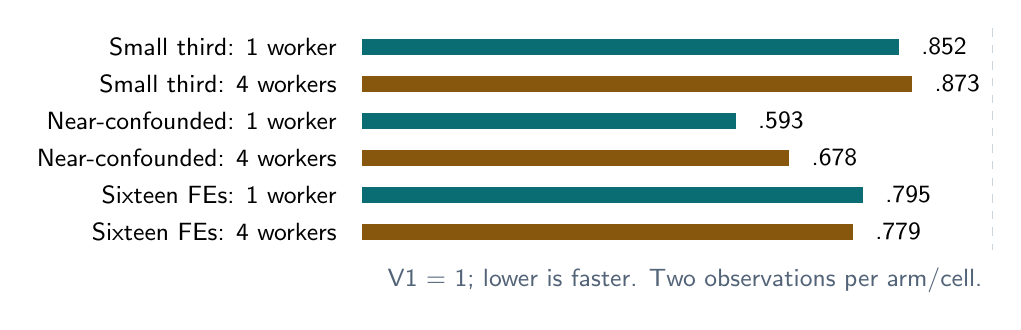
\begin{tikzpicture}[x=8cm,y=.47cm,font=\sffamily\fontsize{8.6}{10.5}\selectfont]
\draw[Rule,dashed] (1,.5) -- (1,-5.5);
\foreach \y/\label/\value/\shade in {0/Small third: 1 worker/.852/Teal,-1/Small third: 4 workers/.873/Amber,-2/Near-confounded: 1 worker/.593/Teal,-3/Near-confounded: 4 workers/.678/Amber,-4/Sixteen FEs: 1 worker/.795/Teal,-5/Sixteen FEs: 4 workers/.779/Amber}{
 \node[anchor=east] at (-.025,\y) {\label};
 \fill[\shade] (0,\y-.22) rectangle (\value,\y+.22);
 \node[anchor=west] at ({\value+.02},\y) {\value};
}
\node[anchor=east,text=Muted] at (1,-6.3) {V1 = 1; lower is faster. Two observations per arm/cell.};
\end{tikzpicture}
\end{center}
\vspace{-7pt}
\begin{center}
\begin{tabular}{lrrrr}
\toprule
 & \multicolumn{2}{c}{\textbf{1 worker, ms}} & \multicolumn{2}{c}{\textbf{4 workers, ms}}\\
\textbf{Revealed A case} & \textbf{V1} & \textbf{Unseeded} & \textbf{V1} & \textbf{Unseeded}\\
\midrule
Small third FE & 263.9 & 225.0 & 120.7 & 105.4\\
Near-confounded third FE & 149.0 & 88.3 & 61.5 & 41.7\\
Sixteen FEs & 849.4 & 675.5 & 360.3 & 280.6\\
\bottomrule
\end{tabular}
\end{center}
\vspace{-5pt}
\sub{More LSMR work can still mean less total work}
All six cells improve descriptively, by about 13--41\%. Unseeded LSMR performs more session work on the small-third and sixteen-FE cases, but saves more prefix work. The sixteen-FE four-worker main action falls from 235 to 182 ms. Its final one-RHS action also falls from 49 to 23 ms: seven unseeded LSMR iterations with an already prepared backend beat four certified MAP sweeps. A small iteration count alone is not a cost comparison.

\textbf{RHS and reuse matter.} The final solve does not pay the main action's backend construction again. This result therefore supports preserving preparation across actions; it does not prove that LSMR is cheapest for an isolated, cold one-RHS request. Descriptive ratios of one-worker to four-worker native medians for this control are about 2.1--2.4.

\begin{note}\smallbody
\textbf{Next policy question.} Test strict unseeded LSMR as the simpler general-FE candidate across the full declared domain. Keep the two-FE CMG construction/core/RHS payback problem separate. These three revealed cases cannot establish a universal winner, a new SCC shortlist, or Mac release performance.
\end{note}
\begin{binding}\tinybody
\textbf{Evidence boundary.} Independent Astra high raw review reruns all 24 original oracle/model checks and verifies 12 exact repeat pairs, cross-worker discrete decisions and resource limits. There are two instrumented observations per arm/cell, fixed V1/control/control/V1 order, no warmups and approximately one-core \code{suggestd} activity throughout. All observations remain included. Logging overhead differs by route, and the first cell spans a reader-repair pause. The original reader failed after successful call 0 because its action summary follows the timed scope. A reviewed continuation revalidated that result and ran only calls 1--23, finishing at 22:12 UTC within the original 22:28 UTC deadline. Every numerical array and failure is retained; no solve was repeated. No qualification or public activation follows.
\end{binding}
\anchor{Private control patch \code{ed404864}; plugin \code{eed24ef2}; plan \code{6deb3796}; continuation \code{fcb88de2}; result \code{b5fd6c41}; independent raw review \code{2636d8e9}. Current evidence: \code{docs/VALIDATION.md} and the compact controlled-results JSON.}
\clearpage

% PAGE 30 / independently reviewed CMG graph substages.
\smallbody
\sect{CMG CONSTRUCTION / 16 OCTOBER}{The serial census is the largest stage}
\tagline{Eight fixed calls; two revealed two-FE cases; exact numerical and work replay.}
A second observational patch splits graph construction into three disjoint stages. The values below are medians of two instrumented observations per cell. They describe elapsed costs; they are not estimates of the speedup an optimization will achieve.

\sub{High-degree weak graph construction, milliseconds}
\begin{center}
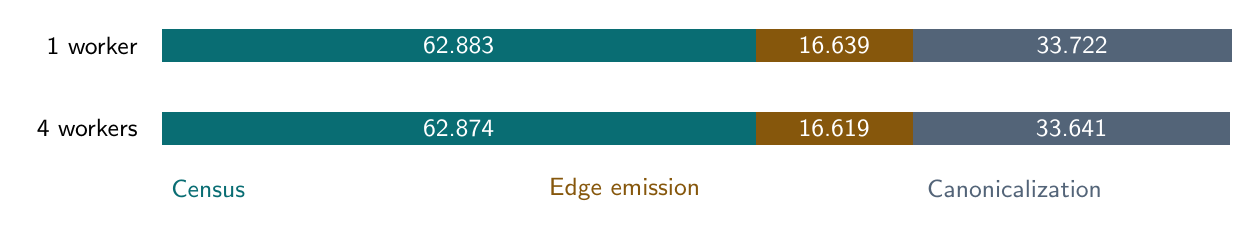
\begin{tikzpicture}[x=.12cm,y=.7cm,font=\sffamily\fontsize{9}{11}\selectfont]
\foreach \y/\label/\a/\b/\c in {0/1 worker/62.883/16.639/33.722,-1.5/4 workers/62.874/16.619/33.641}{
 \node[anchor=east] at (-1.5,\y) {\label};
 \fill[Teal] (0,\y-.3) rectangle (\a,\y+.3);
 \fill[Amber] (\a,\y-.3) rectangle ({\a+\b},\y+.3);
 \fill[Muted] ({\a+\b},\y-.3) rectangle ({\a+\b+\c},\y+.3);
 \node[text=white] at ({\a/2},\y) {\a};
 \node[text=white] at ({\a+\b/2},\y) {\b};
 \node[text=white] at ({\a+\b+\c/2},\y) {\c};
}
\node[anchor=west,text=Teal] at (0,-2.6) {Census};
\node[anchor=west,text=Amber] at (40,-2.6) {Edge emission};
\node[anchor=west,text=Muted] at (80,-2.6) {Canonicalization};
\end{tikzpicture}
\end{center}
\vspace{-6pt}
\begin{center}
\begin{tabular}{lrrrr}
\toprule
 & \multicolumn{2}{c}{\textbf{Weak, ms}} & \multicolumn{2}{c}{\textbf{High-degree weak, ms}}\\
\textbf{Phase} & \textbf{1 worker} & \textbf{4 workers} & \textbf{1 worker} & \textbf{4 workers}\\
\midrule
Census & 7.904 & 7.719 & 62.883 & 62.874\\
Edge emission & 0.854 & 0.854 & 16.639 & 16.619\\
Canonicalization & 3.517 & 3.393 & 33.722 & 33.641\\
Whole graph (inclusive) & 12.631 & 12.291 & 113.663 & 113.572\\
Hierarchy & 4.491 & 4.351 & 35.382 & 35.356\\
CMG cycles, all actions & 2.484 & 2.426 & 16.679 & 16.666\\
\bottomrule
\end{tabular}
\end{center}
\vspace{-5pt}
\sub{What to optimize next}
Census accounts for about 55\% of high-degree graph construction. It loads and sorts worker cells, merges weights with compensated sums, caches canonical cells and joins components. Canonicalization adds about 30\%, including validation, global edge sorting, merging and allocations. Neither timer isolates sorting alone. The parent includes the three stages plus other work; do not add parent and children.

The high-degree census crosses 5.45 million admitted work/allocation boundaries. A synchronous builder passes an always-Continue callback through the same interface used for externally controlled construction. Inspect optimized code before attempting to remove redundant dispatch: fat LTO may already eliminate it. Any specialization must preserve every cancellation checkpoint, work charge, ordinal, refusal and controlled callback. The count is not an instruction count or measured callback latency.

\begin{note}\smallbody
\textbf{Routing implication.} In these observations, four workers reduce other solve time while these construction stages remain serial. More RHS can amortize setup, but worker count alone is not a payback rule. Reduce avoidable construction cost before changing the admission or upgrade policy; the existing numerical and resource contract stays binding.
\end{note}
\begin{binding}\tinybody
\textbf{Evidence boundary.} Eight fresh independent oracle/model checks, four exact repeat pairs, cross-worker agreement, original V1 fingerprints, resource limits and all 3,071 bindings pass independent Astra high review. The fixed eight calls finish in 83.932 seconds, with no retries or exclusions. Source-only integration is inherited; the new native build/ABI checks pass. A superseded auxiliary test-log reference remains discrepant and explicitly recorded; actual code, live tests and the executed plan are independently bound. Ordinary OS activity and instrument overhead remain. No speed qualification, public activation, new shortlist, B or C measurement follows.
\end{binding}
\anchor{Patch \code{24c3d17d}; plugin \code{91af5727}; plan \code{4be88d06}; result \code{9ced797c}; raw review \code{c33d99f3}. Eight observations and exact counters: compact controlled-results JSON.}
\clearpage

% PAGE 31 / exact synchronous-controller causal diagnostic.
\smallbody
\sect{CMG CONSTRUCTION / 16 OCTOBER}{Removing the dummy callback pays off}
\tagline{Sixteen fixed paired calls; exact scientific and work replay; public Auto unchanged.}
Optimized code still packed a 48-byte boundary and invoked an always-Continue external callback at each synchronous work gate. The candidate makes that controller optional. It preserves every interrupt check, validation, budget comparison, ordinal and work charge; controlled and overlap construction keep their callbacks. Candidate disassembly confirms the absent-controller branch skips packing and indirect dispatch.

\sub{Ratio of complete native-time medians: candidate / baseline}
\begin{center}
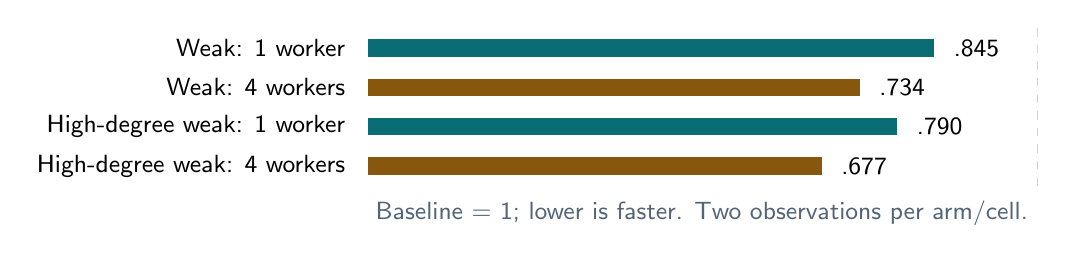
\begin{tikzpicture}[x=8.5cm,y=.5cm,font=\sffamily\fontsize{8.8}{11}\selectfont]
\draw[Rule,dashed] (1,.5) -- (1,-3.5);
\foreach \y/\label/\value/\shade in {0/Weak: 1 worker/.845/Teal,-1/Weak: 4 workers/.734/Amber,-2/High-degree weak: 1 worker/.790/Teal,-3/High-degree weak: 4 workers/.677/Amber}{
 \node[anchor=east] at (-.02,\y) {\label};
 \fill[\shade] (0,\y-.22) rectangle (\value,\y+.22);
 \node[anchor=west] at ({\value+.015},\y) {\value};
}
\node[anchor=east,text=Muted] at (1,-4.2) {Baseline = 1; lower is faster. Two observations per arm/cell.};
\end{tikzpicture}
\end{center}
\vspace{-7pt}
\begin{center}
\begin{tabular}{lrrrr}
\toprule
 & \multicolumn{2}{c}{\textbf{Native solve, ms}} & \multicolumn{2}{c}{\textbf{Graph construction, ms}}\\
\textbf{Revealed A case} & \textbf{Baseline} & \textbf{Candidate} & \textbf{Baseline} & \textbf{Candidate}\\
\midrule
Weak, 1 worker & 67.746 & 57.241 & 12.371 & 4.958\\
Weak, 4 workers & 43.325 & 31.782 & 12.410 & 4.922\\
High-degree weak, 1 worker & 422.487 & 333.654 & 113.514 & 46.359\\
High-degree weak, 4 workers & 276.618 & 187.220 & 113.748 & 46.475\\
\bottomrule
\end{tabular}
\end{center}
\vspace{-5pt}
\sub{A serial cost explains the larger four-worker gain}
Graph construction falls by about 59--60\%. High-degree hierarchy construction also falls from about 35.4 to 14.2 ms, while CMG cycle time stays near 16.7 ms. These disjoint setup scopes explain most of the roughly 89 ms complete-solve reduction. Do not add the graph's child scopes again. The descriptive one-worker/four-worker native ratio improves from 1.53 to 1.78 on high-degree weak, and from 1.56 to 1.80 on weak.

\begin{note}\smallbody
\textbf{Next candidate.} Combine this exact construction change with strict unseeded LSMR for general categorical FEs, keeping the current checkpoint, sampling and work budgets. Test the stable combined artifact across the full domain before adding core or RHS thresholds. More RHS still amortize setup, but these four cells do not establish a payback rule. Never multiply these Mac ratios by earlier Linux ratios.
\end{note}
\begin{binding}\tinybody
\textbf{Evidence boundary.} Fixed baseline/candidate/candidate/baseline within each cell; 16 calls, 120 s each, 1,800 s inclusive, no warmups/retries/exclusions. The runner reports 446.566 s from outer entry, before observer teardown. Independent Astra high review verifies 16 original oracle/model checks, exact four-way science/work/counters, repeat pairs, cross-worker decisions, 32 action caps and every binding. Ordinary desktop activity remains, including approximately one-core \code{suggestd}; both observations per arm remain included. The controller source suite and instrumented native build/ABI pass. Diagnostic validation combines that suite, retained private evidence and reversible clocks. The subsequently combined experimental source passes a fresh 1,934-test Rust suite plus 255 Python and seven portable checks; its uninstrumented native build remains pending. No installed-package admission, release qualification, new SCC discovery or B/C evidence follows.
\end{binding}
\anchor{Controller patch \code{0b3c7fcd}; candidate plugin \code{fec86539}; plan \code{9f2cff08}; result \code{39fb3ed4}; raw review \code{93c2edf1}. Exact data, validation scope and preserved prior failures: compact controlled-results JSON and \code{docs/VALIDATION.md}.}
\clearpage

\end{compactleaf}

% PAGE 32 / prospective combined-candidate discovery.
\begin{compactleaf}
\smallbody
\sect{31 / NEXT DISCOVERY}{One combined candidate, six isolated nodes}
\tagline{Prospective experiment on revealed A cases; no new shortlist or qualification yet.}
\sub{What changes, and what the experiment can establish}
The candidate combines the exact synchronous CMG construction optimization with strict unseeded LSMR for general categorical FEs. Checkpoint, sampling and work budgets stay fixed. It faces the qualified baseline and the complete existing mathematical comparator frontier on all 42 A cells: 21 families at one and four workers. These are known discovery cases; their earlier measurements and optional availability are not reused.

\sub{Three repetitions, each divided into two fixed family groups}
\begin{center}
\begin{tabular}{lrrr}
\toprule
\textbf{Partition per round} & \textbf{Cells} & \textbf{Call cap} & \textbf{Budget, s}\\
\midrule
First 10 sorted families & 20 & 1,274 & 7,280\\
Remaining 11 families & 22 & 1,246 & 7,120\\
\bottomrule
\end{tabular}
\end{center}
Each family keeps both worker counts and all solver alternatives on the same allocation. Three repetitions of each partition require six distinct physical hosts, each with verified full-node isolation. The partitions contain 182 and 178 arm-cell slots. Budgets are proportional to these counts and include cleanup. The design retains at most 7,560 native calls and 43,200 allocation-seconds overall; partitioning does not renew the original budget on every node.

Scientific decisions must agree across worker counts. Solver-route differences are recorded separately: workspace admission and Low-mode chunk aggregation can legitimately change execution metadata. Existing strict CMG/IT contracts and fixed-worker repeatability still apply.

\sub{What remains fixed}
Every available arm receives two fresh scientific prerequisite calls, one traced call, one warmup and three measurements per host. The per-call cap remains 120 seconds. No measurement replacement, partition reassignment or favorable partial aggregate is allowed. Only complete accounting, science, exact local repeats, stable cross-host decisions and strict isolation across all six allocations admit the aggregate. Existing baseline-violation and worst-normalized-ratio rules can still return baseline only.

\begin{note}\smallbody
\textbf{Scaling interpretation.} Each cell has three independent host repetitions and nine measured slots, not nine independent replicates. One- and four-worker comparisons stay paired within a host. Different families may now use different hosts within a logical round; do not interpret that round as one common host for uncertainty. Six nodes may shorten execution, but queue delays and family-cost imbalance remain.
\end{note}
\sub{Release boundary}
Frozen source \code{020eab1e} passes its source-only suite. Both private Mac builds pass their audits and host ABI checks. Linux builds, harness recovery, admission, input binding and plan sealing now pass; the earlier harness and assembly failures remain recorded. Independent Astra review verifies the actual plans, all 447 frozen bindings and the seven scheduled job identities, resources and dependencies. Collectors \code{8153231}--\code{8153236} were released once after fresh hold checks; finalizer \code{8153237} depends on all six. At 02:50 UTC on 17 October the collectors are queued. No new timing result or shortlist is established. Public Auto stays unchanged. Only a valid independently reviewed shortlist admits fresh Mac B12 selection, reviewed activation and equivalence, then untouched C24 confirmation. Earlier V1 discovery and Mac B remain closed NO-GO.

\textbf{RHS coverage limit.} The panel includes a wide-RHS case but no matched cold-single-RHS, reused-single-RHS and wide-batch comparison on one topology. It cannot yet establish a general RHS payback rule. The earlier fast final one-RHS action reused an existing backend.
\clearpage
\end{compactleaf}

\end{document}
